
% ----------------------------------------------------------------------
%                   LATEX TEMPLATE FOR PhD THESIS
% ----------------------------------------------------------------------

% based on Harish Bhanderi's PhD/MPhil template, then Uni Cambridge
% http://www-h.eng.cam.ac.uk/help/tpl/textprocessing/ThesisStyle/
% corrected and extended in 2007 by Jakob Suckale, then MPI-CBG PhD programme
% and made available through OpenWetWare.org - the free biology wiki


%: Style file for Latex
% Most style definitions are in the external file PhDthesisPSnPDF.
% In this template package, it can be found in ./Latex/Classes/
\documentclass[twoside,11pt]{Latex/Classes/PhDthesisPSnPDF}

\makeatletter
        \setlength{\@fptop}{0pt}
\makeatother


%: Macro file for Latex
% Macros help you summarise frequently repeated Latex commands.
% Here, they are placed in an external file /Latex/Macros/MacroFile1.tex
% An macro that you may use frequently is the figuremacro (see introduction.tex)
\include{Latex/Macros/MacroFile1}
%% The amssymb package provides various useful mathematical symbols
\usepackage{amssymb}

%% The amsthm package provides extended theorem environments
\usepackage{amsthm}

%% amsmath for math environment
\usepackage{amsmath}

\DeclareMathOperator*{\argmin}{arg\,min}
\DeclareMathOperator*{\argmax}{arg\,max}
\DeclareMathOperator*{\sign}{sign}

% to break equation
%\usepackage{mathpazo}
%\usepackage{mathptmx}
%\usepackage[mathpazo]{flexisym}
%\usepackage{breqn}

%% For clever reference
%\usepackage{cleveref}

%% color package
\usepackage{color}

%% figure package
\usepackage{epsf,graphicx}
\usepackage{epstopdf}
\usepackage{subfigure}	
\usepackage{transparent}

%% New environment to have some indent inside enumerate environment
\usepackage{enumitem}

%% To create acronym for proper glossary
\usepackage{acro}

%% To number the line in the article
\usepackage{lineno}

%% Environment to include table with notes
\usepackage{array}
\usepackage{threeparttable}
\usepackage{multirow}

%% In order to change size of margin
\usepackage{geometry}
\usepackage{changepage}

%% Colorpackage for table
\usepackage{colortbl}
\usepackage[table]{xcolor}
\usepackage{tabularx}
\usepackage{arydshln}

%% To use URL referencing
\usepackage[hidelinks]{hyperref}

%% In order to draw some graphs
\usepackage{tikz,xifthen}
\usepackage{tikz-qtree}
\usetikzlibrary{decorations.pathmorphing} % noisy shapes
\usetikzlibrary{fit}					% fitting shapes to coordinates
\usetikzlibrary{backgrounds}	% drawing the background after the foreground
\usetikzlibrary{shapes,arrows,shadows}
\usetikzlibrary{calc,decorations.pathreplacing,decorations.markings,positioning}
\usetikzlibrary{snakes,decorations.text,shapes,patterns}
%\usepackage{scalefnt,lmodern,booktabs}

%% Paxkage for cross and tick symbols
\usepackage{pifont}
\newcommand{\cmark}{\large \color{green!60!black!80}\ding{51}}
\newcommand{\mmark}{\large {\color{green!60!black!80}\ding{51}}$^{!}$}
\newcommand{\xmark}{\large \color{red!60!black!80}\ding{55}}
\newcommand{\cmarksmall}{\color{green!60!black!80}\ding{51}}
\newcommand{\mmarksmall}{{\color{green!60!black!80}\ding{51}}$^{!}$}
\newcommand{\xmarksmall}{\color{red!60!black!80}\ding{55}}

\definecolor{autoGuided}{rgb}{ 0.3765    0.7294    0.9412}
\newcommand{\autoGuidedColor}{(light-Blue)}
\definecolor{fullyAuto}{rgb}{ 0.0941    0.3843    0.6627}
\newcommand{\fullyAutoColor}{(dark-blue)}
\definecolor{semiAuto}{rgb}{ 0.0784    0.5059    0.1686}
\newcommand{\semiAutoColor}{(light-green)}
\definecolor{fullyGuided}{rgb}{ 0.4275    0.6902    0.3176}
\newcommand{\fullyGuidedColor}{(dark-green)}

%\acrodef{cap}[CaP]{prostate cancer}
\DeclareAcronym{cap}{
short = CaP,
long = prostate cancer
}
%\acrodef{cade}[CADe]{computer-aided detection}
\DeclareAcronym{cade}{
short = CADe,
long = computer-aided detection
}
%\acrodef{cadx}[CADx]{computer-aided diagnosis}
\DeclareAcronym{cadx}{
short = CADx,
long = computer-aided diagnosis
}
%\acrodef{us}[US]{ultrasound}
\DeclareAcronym{us}{
short = US,
long = ultrasound
}
%\acrodef{ct}[CT]{computer tomography}
\DeclareAcronym{ct}{
short = CT,
long = computer tomography
}
%\acrodef{cad}[CAD]{computer-aided detection and diagnosis}
\DeclareAcronym{cad}{
short = CAD,
long = computer-aided detection and diangosis
}
%\acrodef{mri}[MRI]{magnetic resonance imaging}
\DeclareAcronym{mri}{
short = MRI,
long = magnetic resonance imaging
}
%\acrodef{nmr}[NMR]{nuclear magnetic resonance}
\DeclareAcronym{nmr}{
short = NMR,
long = nuclear magnetic resonance
}
%\acrodef{t2w}[T$_2$-W]{T$_2$ Weighted}
\DeclareAcronym{t2w}{
short = T$_2$-W,
long = T$_2$ Weighted
}
%\acrodef{dce}[DCE]{dynamic contrast-enhanced}
\DeclareAcronym{dce}{
short = DCE,
long = dynamic contrast-enhanced
}
%\acrodef{dw}[DW]{diffusion weighted}
\DeclareAcronym{dw}{
short = DW,
long = diffusion weighted
}
%\acrodef{mrsi}[MRSI]{magnetic resonance spectroscopy imaging}
\DeclareAcronym{mrsi}{
short = MRSI,
long = magnetic resonance spectroscopy imaging
}
%\acrodef{bph}[BPH]{benign prostatic hyperplasia}
\DeclareAcronym{bph}{
short = BPH,
long = benign prostatic hyperplasia
}
%\acrodef{pz}[PZ]{peripheral zone}
\DeclareAcronym{pz}{
short = PZ,
long = peripheral zone
}
%\acrodef{cz}[CZ]{central zone}
\DeclareAcronym{cz}{
short = CZ,
long = central zone
}
%\acrodef{tz}[TZ]{transitional zone}
\DeclareAcronym{tz}{
short = TZ,
long = transitional zone
}
%\acrodef{cg}[CG]{central gland}
\DeclareAcronym{cg}{
short = CG,
long = central gland
}
%\acrodef{psa}[PSA]{prostate-specific antigen}
\DeclareAcronym{psa}{
short = PSA,
long = prostate-specific antigen
}
%\acrodef{trus}[TRUS]{transrectal ultrasound}
\DeclareAcronym{trus}{
short = TRUS,
long = transrectal ultrasound
}
%\acrodef{tr}[TR]{repetition time}
\DeclareAcronym{tr}{
short = TR,
long = repetition time
}
%\acrodef{te}[TE]{echo time}
\DeclareAcronym{te}{
short = TE,
long = echo time
}
%\acrodef{si}[SI]{signal intensity}
\DeclareAcronym{si}{
short = SI,
long = signal intensity
}
%\acrodef{ees}[EES]{extravascular-extracellular space}
\DeclareAcronym{ees}{
short = EES,
long = extravascular-extracellular space
}
%\acrodef{t1w}[T$_1$-W]{T$_1$ Weighted}
\DeclareAcronym{t1w}{
short = T$_1$-W,
long = T$_1$ Weighted
}
%\acrodef{fse}[FSE]{Fast Spin-Echo}
\DeclareAcronym{fse}{
short = FSE,
long = Fast Spin-Echo
}
%\acrodef{adc}[ADC]{Apparent Diffusion Coeffient}
\DeclareAcronym{adc}{
short = ADC,
long = apparent diffusion coefficient
}
%\acrodef{roi}[ROI]{region of interest}
\DeclareAcronym{roi}{
short = ROI,
long = region of interest
}
%\acrodef{cse}[CSE]{chemical shift effect}
\DeclareAcronym{cse}{
short = CSE,
long = chemical shift effect
}
%\acrodef{snr}[SNR]{signal-to-noise}
\DeclareAcronym{snr}{
short = SNR,
long = signal-to-noise
}
%\acrodef{gs}[GS]{Gleason score}
\DeclareAcronym{gs}{
short = GS,
long = Gleason score
}
%\acrodef{ersspc}[ERSSPC]{European Randomized Study of Screening for Prostate Cancer}
\DeclareAcronym{ersspc}{
short = ERSSPC,
long = European Randomized Study of Screening for Prostate Cancer
}
%\acrodef{plco}[PLCO]{Prostate, Lung, Colorectal and Ovarian}
\DeclareAcronym{plco}{
short = PLCO,
long = Prostate Lung Colorectal and Ovarian
}
%\acrodef{fig}[Fig.]{figure}
\DeclareAcronym{fig}{
short = Fig.,
long = figure
}
\DeclareAcronym{tab}{
short = Tab.,
long = table
}
\DeclareAcronym{eq}{
short = Eq.,
long = equation
}
\DeclareAcronym{sec}{
short = Sect.,
long = section
}
\DeclareAcronym{fov}{
short = FOV,
long = field of view
}
\DeclareAcronym{dwt}{
short = DWT,
long = discrete wavelet transform
}
\DeclareAcronym{dwst}{
short = DWST,
long = discrete wavelet squared transform
}
\DeclareAcronym{map}{
short = MAP,
long = maximum \textit{a posteriori}
}
\DeclareAcronym{ml}{
short = ML,
long = maximum likelihood
}
\DeclareAcronym{mrf}{
short = MRF,
long = Markov random field
}
\DeclareAcronym{itk}{
short = ITK,
long = Insight Segmentation and Registration Toolkit
}
\DeclareAcronym{es}{
short = ES,
long = Evolution Strategy
}
\DeclareAcronym{pdf}{
short = PDF,
long = probability density function
}
\DeclareAcronym{gscale}{
short = \textit{g}-scale,
long = generalized scale
}
\DeclareAcronym{aif}{
short = AIF,
long = arterial input function
}
\DeclareAcronym{svd}{
short = SVD,
long = singular value decomposition
}
\DeclareAcronym{mse}{
short = MSE,
long = mean squared error
}
\DeclareAcronym{mi}{
short = MI,
long = mutual information
}
\DeclareAcronym{mantra}{
short = MANTRA,
long = multi-attribute non-initializing texture reconstruction based active shape model
}
\DeclareAcronym{asm}{
short = ASM,
long = active shape model
}
\DeclareAcronym{pca}{
short = PCA,
long = principal components analysis
}
\DeclareAcronym{weritas}{
short = WERITAS,
long = weighted ensemble of regional image textures for active shape model segmentation
}
\DeclareAcronym{staple}{
short = STAPLE,
long = simultaneous truth and performance level estimation
}
\DeclareAcronym{lda}{
short = LDA,
long = linear discriminant analysis
}
\DeclareAcronym{lbp}{
short = LBP,
long = local binary pattern
}
\DeclareAcronym{tps}{
short = TPS,
long = thin plate spline
}
\DeclareAcronym{acm}{
short = ACM,
long = active contour model
}
\DeclareAcronym{cmi}{
short = CMI,
long = combined mutual information
}
\DeclareAcronym{svm}{
short = SVM,
long = support vector machines
}
\DeclareAcronym{rvm}{
short = RVM,
long = relevant vector machine
}
\DeclareAcronym{rbf}{
short = RBF,
long = radial basis function
}
\DeclareAcronym{knn}{
short = $k$-NN,
long = $k$-neareast neighbour
}
\DeclareAcronym{dct}{
short = DCT,
long = discrete cosine transform
}
\DeclareAcronym{hog}{
short = HOG,
long = histogram of oriented gradient
}
\DeclareAcronym{dft}{
short = DFT,
long = discrete fourier transform
}
\DeclareAcronym{mrmr}{
short = mRMR,
long = minimum redundancy maximum relevance
}
\DeclareAcronym{lle}{
short = LLE,
long = locally linear embedding
}
\DeclareAcronym{ica}{
short = ICA,
long = independent components analysis
}
\DeclareAcronym{qda}{
short = QDA,
long = quadratic discriminant analysis
}
\DeclareAcronym{id3}{
short = ID3,
long = iterative dichotomiser 3
}
\DeclareAcronym{cart}{
short = CART,
long = classification and regression tree
}
\DeclareAcronym{bagging}{
short = bagging,
long = bootsrap aggregating
}
\DeclareAcronym{loo}{
short = LOOCV,
long = leave-one-out cross-validation
}
\DeclareAcronym{kcv}{
short = $k$-CV,
long = $k$-fold cross-validation
}
\DeclareAcronym{roc}{
short = ROC,
long = receiver operating characteristic
}
\DeclareAcronym{froc}{
short = FROC,
long = free-response receiver operating characteristic
}
\DeclareAcronym{auc}{
short = AUC,
long = area under the curve
}



%: ----------------------------------------------------------------------
%:                  TITLE PAGE: name, degree,..
% ----------------------------------------------------------------------
% below is to generate the title page with crest and author name

%if output to PDF then put the following in PDF header
\ifpdf  
    \pdfinfo { /Title  (Computer-Aided Diagnosis for Prostate Cancer using Multi-Parametric Magnetic Resonance Imaging)
               /Creator (TeX)
               /Producer (pdfTeX)
               /Author (Guillaume Lemaitre g.lemaitre58@gmail.com)
               /CreationDate (D:201610151200ss)  %format D:YYYYMMDDhhmmss
               /ModDate (D:201610151200ss)
               /Subject (PhD Dissertation of Guillaume Lemaitre)
               /Keywords (CAD, mp-MRI, spectroscopy, MRI) }
    \pdfcatalog { /PageMode (/UseOutlines)
                  /OpenAction (fitbh)  }
\fi


\title{Computer-Aided Diagnosis for Prostate Cancer using Multi-Parametric Magnetic Resonance Imaging}



% ----------------------------------------------------------------------
% The section below defines www links/email for author and institutions
% They will appear on the title page of the PDF and can be clicked
\ifpdf
  \author{\href{mailto:guillaume.lemaitre@udg.edu}{Guillaume Lema\^itre}}
%  \cityofbirth{born in XYZ} % uncomment this if your university requires this
%  % If city of birth is required, also uncomment 2 sections in PhDthesisPSnPDF
%  % Just search for the "city" and you'll find them.
  % The crest is a graphics file of the logo of your research institution.
  % Place it in ./0_frontmatter/figures and specify the width

%% First university
  \firstlab{\href{http://le2i.cnrs.fr/}{LE2I}}
  \firstlogolab{
\includegraphics[width=2cm]{logos/logole2i.eps}}
  \firstuni{\href{http://www.u-bourgogne.fr/}{Universit\'e de Bourgogne}}
  \firstlogouni{\includegraphics[width=2cm]{logos/logo-ub-no-bg.pdf}}

  
%% Second university
  \secondlab{\href{http://vicorob.udg.es/}{ViCOROB}}
  \secondlogolab{\includegraphics[width=2cm]{logos/vicorobLogo1.png}}

  \seconduni{\href{https://www.udg.edu/}{Universitat de Girona}}
  \secondlogouni{\includegraphics[scale =0.5]{logos/UdG_dues_linies_centrat_blau.png}}

  \supervisora{Fabrice M\'eriaudeau (LE2I/CISIR - UBFC/UTP)}
  \supervisorb{Robert Mart\'i Marly (ViCOROB - UdG)}
  \supervisorc{Jordi Freixenet Bosch (ViCOROB - UdG)}
  \supervisord{Paul Michael Walker (LE2I - UBFC)}  
  
% If you are not creating a PDF then use the following. The default is PDF.
\else
  \author{Guillaume Lema\^itre}
%  \cityofbirth{born in XYZ}
%% First university
  \firstlab{\href{http://le2i.cnrs.fr/}{LE2I}}
  \firstlogolab{
\includegraphics[width=2cm]{logos/logole2i.eps}}
  \firstuni{\href{http://www.u-bourgogne.fr/}{Universit\'e de Bourgogne}}
  \firstlogouni{
\includegraphics[width=2cm]{logos/logoubblue.eps}}
  
%% Second university
  \secondlab{\href{http://vicorob.udg.es/}{ViCOROB}}
  \secondlogolab{
\includegraphics[width=2cm]{logos/logovicorob.eps}}
  \seconduni{\href{https://www.udg.edu/}{Universitat de Girona}}
  \secondlogouni{
\includegraphics[width=2cm]{logos/logoudg.eps}}
  
  
  \supervisora{Fabrice M\'eriaudeau (LE2I/CISIR - UBFC/UTP)}
  \supervisorb{Robert Mart\'i Marly (ViCOROB - UdG)}
  \supervisorc{Jordi Freixenet Bosch (ViCOROB - UdG)}
  \supervisord{Paul Michael Walker (LE2I - UBFC)}
\fi

%\renewcommand{\submittedtext}{change the default text here if needed}
\degree{Philosophi\ae Doctor (PhD)}
\degreedate{November 2016}


% ----------------------------------------------------------------------
       
% turn of those nasty overfull and underfull hboxes
\hbadness=10000
\hfuzz=50pt


%: --------------------------------------------------------------
%:                  FRONT MATTER: dedications, abstract,..
% --------------------------------------------------------------
\onehalfspacing
%\DeclareInstance{acro-title}{empty}{sectioning}{name-format =}
\begin{document}

%\language{english}

% sets line spacing
%\renewcommand\baselinestretch{1.2}
\baselineskip=18pt plus1pt


%: ----------------------- generate cover page ------------------------

\maketitle  % command to print the title page with above variables

%: ----------------------- cover page back side ------------------------
% Your research institution may require reviewer names, etc.
% This cover back side is required by Dresden Med Fac; uncomment if needed.

\newpage
{\pagestyle{plain}
\vspace{10mm}
Reviewers:

\begin{itemize}
\item[] Su Ruan, Professor at Universit\'e de Rouen - LITIS
\item[] Reyer Zwiggelaar, Professor at Aberystwyth Universtiy - Vision, Graphics, and Visualisation Group
%\item[] Soumya Ghose, Research Associate at Case Western Reserve University
\end{itemize}

\vspace{20mm}
Day of the defense: 28 November 2016

\vspace{20mm}
\hspace{70mm}Signature from head of PhD committee:



%: ----------------------- abstract ------------------------

% Your institution may have specific regulations if you need an abstract and where it is to be placed in the document. The default here is just after title.

%
% Thesis Abstract -----------------------------------------------------


%\begin{abstractslong}    %uncommenting this line, gives a different abstract heading
\begin{abstracts}        %this creates the heading for the abstract page
Prostate cancer (CaP) is the second most diagnosed cancer in men all over the world.
CaP growth is characterized by two main types of evolution: (i) the slow-growing tumours progress slowly and usually remain confined to the prostate gland; (ii) the fast-growing tumours metastasize from prostate gland to other organs, which might lead to incurable diseases.
Therefore, early diagnosis and risk assessment play major roles in patient treatment and follow-up.
In the last decades, new imaging techniques based on Magnetic Resonance Imaging (MRI) have been developed improving diagnosis.
In practise, diagnosis can be affected by multiple factors such as observer variability and visibility and complexity of the lesions.
In this regard, computer-aided detection and computer-aided diagnosis systems are being designed to help radiologists in their clinical practice.

Our research extensively analyzes the current state-of-the-art in the development of computer-aided diagnosis and detection systems for prostate cancer detection.
Currently, no computer-aided system using all available MRI modalities has been proposed and tested on a common dataset.
Therefore, we propose a new computer-aided system taking advantage of all MRI modalities (i.e., \acs*{t2w}-\acs*{mri}, \acs*{dce}-\acs*{mri}, DW-\acs*{mri}, \acs*{mrsi}).
Particular attention is paid to the normalization of the \acs*{mri} modalities prior to develop our computer-aided system.
This system has been extensively tested on a dataset which has been made publicly available.
\end{abstracts}
%\end{abstractlongs}
%-------------------------------------------------------------------------

\begin{abstractCatalan}

El c\`ancer de pr\`ostata (CaP) \'es el segon c\`ancer m\'es diagnosticat en homes a tot el m\'on.
El creixement del CaP es caracteritza per dos tipus principals d'evoluci\'o: (i) els tumors de creixement lent que progressen lentament i en general romanen confinats en la gl\`andula de la pr\`ostata; (ii) els tumors de creixement r\`apid que desenvolupen met\`astasi de la pr\`ostata a altres \`organs, el que podria conduir a malalties incurables.
Conseq\"uentment, el diagn\`ostic preco\c{c} i l'avaluaci\'o del risc exerceixen un paper important en el tractament del pacient i el seguiment.
En les \'ultimes d\`ecades s'han desenvolupat noves t\`ecniques d'imatge basades en imatge de resson\`ancia magn\`etica (RM, o MRI de l'angl\`es) per millorar el diagn\`ostic.
A la pr\`actica, el diagn\`ostic pot ser afectat per diversos factors com ara la variabilitat de l'observador i la visibilitat i la complexitat de les lesions.
En aquest sentit, s'estan desenvolupant sistemes per a l'ajuda a la detecci\'o i diagn\`ostic per ordinador per ajudar els radi\`olegs en la seva pr\`actica cl\'inica.

La nostra recerca analitza \`ampliament l'estat de l'art en el desenvolupament de sistemes per a l'ajuda a la detecci\'o i diagn\`ostic per ordinador per a la detecci\'o del c\`ancer de pr\`ostata.
En l'actualitat, no hi ha cap sistema d'ajuda al diagn\`ostic que utilitzi totes les modalitats de MRI disponibles i que hagi estat avaluat en un conjunt de dades com\'u.
Per tant, proposem un nou sistema d'ajuda al diagn\`ostic per ordinador aprofitant totes les modalitats de resson\`ancia magn\`etica (\'es a dir \acs*{t2w}-MRI, DCE-MRI, DW-MRI, MRSI).
Com a etapa pr\`evia al desenvolupament del sistema, es presta especial atenci\'o a la normalitzaci\'o de les modalitats de resson\`ancia magn\`etica.
El sistema desenvolupat ha estat avaluat extensivament en un conjunt de dades que s'han posat a disposici\'o p\'ublica.
 
\end{abstractCatalan}

% ---------------------------------------------------------------------- 
\begin{abstractSpanish}

El c\'ancer de pr\'ostata (CaP) es el segundo c\'ancer m\'as diagn\'osticado en hombres en todo el mundo.
El crecimiento del CaP se caracteriza por dos tipos principales de evoluci\'on: (i) los tumores de crecimiento lento que progresan lentamente y por lo general permanecen confinados en la gl\'andula de la pr\'ostata; (ii) los tumores de crecimiento r\'apido que desarrollan met\'astasis de la pr\'ostata a otros \'organos, lo que podr\'ia conducir a enfermedades incurables.
Consecuentemente, el diagn\'ostico precoz y la evaluaci\'on del riesgo desempe\~nan un papel importante en el tratamiento del paciente y el seguimiento. En las \'ultimas d\'ecadas se han desarrollado  nuevas t\'ecnicas de imagen basadas en imagen de resonancia magn\'etica (RM, o MRI del ingl\'es) para mejorar el diagn\'ostico. En la pr\'actica, el diagn\'ostico puede ser afectado por varios factores tales como la variabilidad del observador y la visibilidad y la complejidad de las lesiones.
En este sentido, se est\'an desarrollando sistemas para la ayuda a la detecci\'on y diagn\'ostico por ordenador para ayudar a los radi\'ologos en su pr\'actica cl\'inica.

Nuestra investigaci\'on analiza ampliamente el estado del arte en el desarrollo de sistemas para la ayuda a la detecci\'on y diagn\'ostico por ordenador para la detecci\'on del c\`ancer de pr\'ostata.
En la actualidad, no existe ning\'un sistema de ayuda al diagn\'ostico que utilice todas las modalidades de MRI disponibles y que haya sido evaluado en un conjunto de datos com\'un.
Por lo tanto, proponemos un nuevo sistema de ayuda al diagn\'ostico por ordenador aprovechando todas las modalidades de resonancia magn\'etica (es decir T2W-MRI, DCE-MRI, DW-MRI, MRSI).
Como etapa previa al desarrollo del sistema, se presta especial atenci\'on a la normalizaci\'on de las modalidades de resonancia magn\'etica.
El sistema desarrollado ha sido evaluado extensivamente en un conjunto de datos que se han puesto a disposici\'on p\'ublica.
 
\end{abstractSpanish}

%-------------------------------------------------------------------------
\begin{abstractFrench}

Le cancer de la prostate est le second type de cancer le plus diagnostiqu\'e au monde.
Il est caract\'eris\'e par deux evolutions distinctes : (i) les tumeurs \`a croissances lentes progressent lentement et restent g\'en\'eralement confin\'ees dans la glande prostatique; (ii) les tumeurs \`a croissances rapides se m\'etastasent de la prostate \`a d'autres organes p\'eriph\'eriques, pouvant causer le d\'evelopement de maladies incurables.
C'est pour cela qu'un diagnostic pr\'ecoce et une \'evaluation du risque jouent des r\^oles majeurs dans le traitement et le suivi du patient.
Durant la derni\`ere d\'ec\'enie, de nouvelles m\'ethodes d'imagerie bas\'ees sur l'Imagerie par R\'esonance Magn\'etique (IRM) ont \'et\'e d\'evelop\'ees.
En pratique, le diagnostic clinique peut \^etre affect\'e par de multiples facteurs comme la variabilit\'e entre observateurs et la complexit\'e des l\'esions lues.
Pour ce faire, des syst\`emes de d\'etection et de diagnostic assist\'e par ordinateur (DAO) ont \'et\'e d\'evelop\'es pour aider les radiologistes durant leurs t\^aches cliniques.

Notre recherche analyse extensivement l'\'etat de l'art actuel concernant le d\'evelopement des syst\`emes de DAO pour la d\'etection du cancer de la prostate.
Actuellement, il n'\'existe aucun syst\`eme de DAO utilisant toutes les modalit\'es IRM disponibles et qui plus est, test\'e sur une base de donn\'ees commune.
Par cons\'equent, nous proposons un nouveau syst\`eme de DAO tirant profit de toutes les modalit\'es IRM (i.e., T2W-MRI, DCE-MRI, DW-MRI, MRSI).
Une attention particuli\`ere est port\'ee sur la normalisation de ces donn\'ees multi-param\'etriques avant la conception du syst\`eme de DAO.
De plus, notre syst\`eme de DAO a \'et\'e test\'e sur une base de donn\'ees que nous rendons publique.

\end{abstractFrench}


% The original template provides and abstractseparate environment, if your institution requires them to be separate. I think it's easier to print the abstract from the complete thesis by restricting printing to the relevant page.
%\begin{abstractseparate}
%  
% Thesis Abstract -----------------------------------------------------


%\begin{abstractslong}    %uncommenting this line, gives a different abstract heading
\begin{abstracts}        %this creates the heading for the abstract page
Prostate cancer (CaP) is the second most diagnosed cancer in men all over the world.
CaP growth is characterized by two main types of evolution: (i) the slow-growing tumours progress slowly and usually remain confined to the prostate gland; (ii) the fast-growing tumours metastasize from prostate gland to other organs, which might lead to incurable diseases.
Therefore, early diagnosis and risk assessment play major roles in patient treatment and follow-up.
In the last decades, new imaging techniques based on Magnetic Resonance Imaging (MRI) have been developed improving diagnosis.
In practise, diagnosis can be affected by multiple factors such as observer variability and visibility and complexity of the lesions.
In this regard, computer-aided detection and computer-aided diagnosis systems are being designed to help radiologists in their clinical practice.

Our research extensively analyzes the current state-of-the-art in the development of computer-aided diagnosis and detection systems for prostate cancer detection.
Currently, no computer-aided system using all available MRI modalities has been proposed and tested on a common dataset.
Therefore, we propose a new computer-aided system taking advantage of all MRI modalities (i.e., \acs*{t2w}-\acs*{mri}, \acs*{dce}-\acs*{mri}, DW-\acs*{mri}, \acs*{mrsi}).
Particular attention is paid to the normalization of the \acs*{mri} modalities prior to develop our computer-aided system.
This system has been extensively tested on a dataset which has been made publicly available.
\end{abstracts}
%\end{abstractlongs}
%-------------------------------------------------------------------------

\begin{abstractCatalan}

El c\`ancer de pr\`ostata (CaP) \'es el segon c\`ancer m\'es diagnosticat en homes a tot el m\'on.
El creixement del CaP es caracteritza per dos tipus principals d'evoluci\'o: (i) els tumors de creixement lent que progressen lentament i en general romanen confinats en la gl\`andula de la pr\`ostata; (ii) els tumors de creixement r\`apid que desenvolupen met\`astasi de la pr\`ostata a altres \`organs, el que podria conduir a malalties incurables.
Conseq\"uentment, el diagn\`ostic preco\c{c} i l'avaluaci\'o del risc exerceixen un paper important en el tractament del pacient i el seguiment.
En les \'ultimes d\`ecades s'han desenvolupat noves t\`ecniques d'imatge basades en imatge de resson\`ancia magn\`etica (RM, o MRI de l'angl\`es) per millorar el diagn\`ostic.
A la pr\`actica, el diagn\`ostic pot ser afectat per diversos factors com ara la variabilitat de l'observador i la visibilitat i la complexitat de les lesions.
En aquest sentit, s'estan desenvolupant sistemes per a l'ajuda a la detecci\'o i diagn\`ostic per ordinador per ajudar els radi\`olegs en la seva pr\`actica cl\'inica.

La nostra recerca analitza \`ampliament l'estat de l'art en el desenvolupament de sistemes per a l'ajuda a la detecci\'o i diagn\`ostic per ordinador per a la detecci\'o del c\`ancer de pr\`ostata.
En l'actualitat, no hi ha cap sistema d'ajuda al diagn\`ostic que utilitzi totes les modalitats de MRI disponibles i que hagi estat avaluat en un conjunt de dades com\'u.
Per tant, proposem un nou sistema d'ajuda al diagn\`ostic per ordinador aprofitant totes les modalitats de resson\`ancia magn\`etica (\'es a dir \acs*{t2w}-MRI, DCE-MRI, DW-MRI, MRSI).
Com a etapa pr\`evia al desenvolupament del sistema, es presta especial atenci\'o a la normalitzaci\'o de les modalitats de resson\`ancia magn\`etica.
El sistema desenvolupat ha estat avaluat extensivament en un conjunt de dades que s'han posat a disposici\'o p\'ublica.
 
\end{abstractCatalan}

% ---------------------------------------------------------------------- 
\begin{abstractSpanish}

El c\'ancer de pr\'ostata (CaP) es el segundo c\'ancer m\'as diagn\'osticado en hombres en todo el mundo.
El crecimiento del CaP se caracteriza por dos tipos principales de evoluci\'on: (i) los tumores de crecimiento lento que progresan lentamente y por lo general permanecen confinados en la gl\'andula de la pr\'ostata; (ii) los tumores de crecimiento r\'apido que desarrollan met\'astasis de la pr\'ostata a otros \'organos, lo que podr\'ia conducir a enfermedades incurables.
Consecuentemente, el diagn\'ostico precoz y la evaluaci\'on del riesgo desempe\~nan un papel importante en el tratamiento del paciente y el seguimiento. En las \'ultimas d\'ecadas se han desarrollado  nuevas t\'ecnicas de imagen basadas en imagen de resonancia magn\'etica (RM, o MRI del ingl\'es) para mejorar el diagn\'ostico. En la pr\'actica, el diagn\'ostico puede ser afectado por varios factores tales como la variabilidad del observador y la visibilidad y la complejidad de las lesiones.
En este sentido, se est\'an desarrollando sistemas para la ayuda a la detecci\'on y diagn\'ostico por ordenador para ayudar a los radi\'ologos en su pr\'actica cl\'inica.

Nuestra investigaci\'on analiza ampliamente el estado del arte en el desarrollo de sistemas para la ayuda a la detecci\'on y diagn\'ostico por ordenador para la detecci\'on del c\`ancer de pr\'ostata.
En la actualidad, no existe ning\'un sistema de ayuda al diagn\'ostico que utilice todas las modalidades de MRI disponibles y que haya sido evaluado en un conjunto de datos com\'un.
Por lo tanto, proponemos un nuevo sistema de ayuda al diagn\'ostico por ordenador aprovechando todas las modalidades de resonancia magn\'etica (es decir T2W-MRI, DCE-MRI, DW-MRI, MRSI).
Como etapa previa al desarrollo del sistema, se presta especial atenci\'on a la normalizaci\'on de las modalidades de resonancia magn\'etica.
El sistema desarrollado ha sido evaluado extensivamente en un conjunto de datos que se han puesto a disposici\'on p\'ublica.
 
\end{abstractSpanish}

%-------------------------------------------------------------------------
\begin{abstractFrench}

Le cancer de la prostate est le second type de cancer le plus diagnostiqu\'e au monde.
Il est caract\'eris\'e par deux evolutions distinctes : (i) les tumeurs \`a croissances lentes progressent lentement et restent g\'en\'eralement confin\'ees dans la glande prostatique; (ii) les tumeurs \`a croissances rapides se m\'etastasent de la prostate \`a d'autres organes p\'eriph\'eriques, pouvant causer le d\'evelopement de maladies incurables.
C'est pour cela qu'un diagnostic pr\'ecoce et une \'evaluation du risque jouent des r\^oles majeurs dans le traitement et le suivi du patient.
Durant la derni\`ere d\'ec\'enie, de nouvelles m\'ethodes d'imagerie bas\'ees sur l'Imagerie par R\'esonance Magn\'etique (IRM) ont \'et\'e d\'evelop\'ees.
En pratique, le diagnostic clinique peut \^etre affect\'e par de multiples facteurs comme la variabilit\'e entre observateurs et la complexit\'e des l\'esions lues.
Pour ce faire, des syst\`emes de d\'etection et de diagnostic assist\'e par ordinateur (DAO) ont \'et\'e d\'evelop\'es pour aider les radiologistes durant leurs t\^aches cliniques.

Notre recherche analyse extensivement l'\'etat de l'art actuel concernant le d\'evelopement des syst\`emes de DAO pour la d\'etection du cancer de la prostate.
Actuellement, il n'\'existe aucun syst\`eme de DAO utilisant toutes les modalit\'es IRM disponibles et qui plus est, test\'e sur une base de donn\'ees commune.
Par cons\'equent, nous proposons un nouveau syst\`eme de DAO tirant profit de toutes les modalit\'es IRM (i.e., T2W-MRI, DCE-MRI, DW-MRI, MRSI).
Une attention particuli\`ere est port\'ee sur la normalisation de ces donn\'ees multi-param\'etriques avant la conception du syst\`eme de DAO.
De plus, notre syst\`eme de DAO a \'et\'e test\'e sur une base de donn\'ees que nous rendons publique.

\end{abstractFrench}

%\end{abstractseparate}


%: ----------------------- tie in front matter ------------------------

% Thesis Dedictation ---------------------------------------------------

\begin{dedication} %this creates the heading for the dedication page
\begin{flushright}
\textit{To my parents,\\
  to my brother and his family,\\
  to my wife,\\
  to those who are dear to my heart,\\
  and all those who find themselves in this work.}
\end{flushright}
\end{dedication}

% ----------------------------------------------------------------------

\begin{publication}

\subsubsection*{Peer-Review Journals Papers}

\begin{enumerate}\scriptsize
\item \textbf{G. Lemaitre, R. Marti, M. Rastgoo, J. Massich, F. Freixenet, J. C. Vilanova, and F. Meriaudeau}, ``Automatic prostate cancer detection through DCE-MRI images: all you need is a good normalization'', \textit{Medical Image Analysis}, Submitted.
\item \textbf{G. Lemaitre, F. Nogueira, and C. Aridas}, ``Imbalanced-learn: A Python Toolbox to Tackle the Curse of Imbalanced Datasets in Machine Learning'', \textit{Journal of Machine Learning Research}, Submitted.
\item \textbf{G. Lemaitre, M. Rastgoo, J. Massich, C. Y. Cheung, T. Y. Wong, E. Lamoureux, D. Milea, F. Meriaudeau, and D. Sidibe}, ``Classification of SD-OCT Volumes using Local Binary Patterns: Experimental Validation for DME detection'', \textit{Journal of Ophthalmology}, vol. 2016, May 2016.
\item \textbf{G. Lemaitre, R. Marti, J. Freixenet, J. C. Vilanova, P. M. Walker, and F. Meriaudeau}, ``Computer-Aided Detection and Diagnosis for prostate cancer based on mono and multi-parametric MRI: A Review'', \textit{Computer in Biology and Medicine}, vol. 60, pp 8 - 31, 2015.
\end{enumerate}

\subsubsection*{Peer-Review International Conferences}

\begin{enumerate}\scriptsize
\item \textbf{G. Lemaitre, M. Rastgoo, J. Massich, J. C. Vilanova, P. M. Walker, J. Freixenet, A. Meyer-Baese, F. Meriaudeau, and R. Marti}, ``Normalization of T2W-MRI prostate images using Rician a priori'', \textit{SPIE Medical Imaging 2016}. San Diego: USA (February 2016).
\item \textbf{G. Lemaitre, M. Rastgoo, J. Massich, S. Sankar, F. Meriaudeau, and D. Sidibe}, ``Classification of SD-OCT volumes with LBP: Application to DME detection'', \textit{Ophthalmic Medical Image Analysis Workshop (OMIA), Medical Image Computing and Computer Assisted Interventions (MICCAI) 2015}. Munich: Germany (Oct. 2015).
\item \textbf{G. Lemaitre, J. Massich, R. Marti, J. Freixenet, J. C. Vilanova, P. M. Walker, D. Sidibe, and F. Meriaudeau}, ``A Boosting Approach for Prostate Cancer Detection using Multi-parametric MRI'', \textit{International Conference on Quality Control and Artificial Vision (QCAV) 2015}. Le Creusot: France (Jun. 2015).
\item \textbf{G. Lemaitre, A. Bikfalvi, J. Llach, J. Massich, and F. Julian}, ``Business Model Design for University Technology Valorisation'', \textit{International Technology, Education and Development Conference (INTED) 2015}. Madrid: Spain (Mar. 2015).
\end{enumerate}

\subsubsection*{Thesis}

\begin{enumerate}\scriptsize
\item \textbf{G. Lemaitre, A. Bikfalvi, and J. Llach}, ``Valorisation of Computerized Technology in the Health Care Sector'', \textit{Thesis for Master in Science Business Innovation and Technology Management (BITM)}, 2014.
\end{enumerate}

\subsubsection*{Contributed Peer-Review Journals Papers}

\begin{enumerate}\scriptsize
\item \textbf{K. Alsaih, G. Lemaitre, J. Massich, M. Rastgoo, D. Sidibe, and F. Meriaudeau}, ``Machine Learning Techniques for DME Classification on SD-OCT images'', \textit{BioMedical Engineering OnLine}, Submitted.
\item \textbf{I. P. Houben, P. Van de Voorde, C. R. Jeukens, J. E. Wildberger, G. Lemaitre, I. A. Illan, A. Meyer-Baese, L. F. Kooreman, M. L. Smidt, and M. B. Lobbes}, ``Contrast-enhanced spectral mammography as work-up tool in patients recalled from breast cancer screening: risks versus benefits'', \textit{European Radiology}, Submitted.
\item \textbf{D. Sidibe, S. Sankar, G. Lemaitre, M. Rastgoo, J. Massich, C. Y. Cheung, G. S. Tan, D. Milea, E. Lamoureux, T. Y. Wong, and F. Meriaudeau}, ``An anomaly detection approach for the identification of DME patients using spectral domain optical coherence tomography images'', \textit{Computer Methods and Programs in Biomedicine}, Submitted.
\item \textbf{M. Belkacemi, C. Stolz, A. Mathieu, G. Lemaitre, J. Massich, and O. Aubreton}, ``Non Destructive Testing based on a Scanning-From-Heating approach: Application to non-through Defect Detection and Fiber Orientation Assessment'', \textit{Journal of Electronic Imaging}, vol. 24(6), pp 1-8, Nov/Dec 2015.
\end{enumerate}

\subsubsection*{Contributed Peer-Review International Conferences Papers}

\begin{enumerate}\scriptsize
\item \textbf{J. Massich, M. Rastgoo, G. Lemaitre, C. Cheung, T. Y. Wong, D. Sidibe, and F. Meriaudeau}, ``Classifying DME vs normal SD-OCT volumes: A review'', \textit{23\textsuperscript{rd} International Conference on Pattern Recognition (ICPR) 2016}. Cancun: Mexico (December 2016).
\item \textbf{K. Alsaih, G. Lemaitre, J. Massich, M. Rastgoo, D. Sidibe, T. Y. Wong, E. Lamoureux, D. Milea, C. Leung, and F. Meriaudeau}, ``Classification of SD-OCT volumes with multi-pyramids, LBP and HoG descriptors: Application to DME detection'', \textit{38\textsuperscript{th} International Conference of the IEEE Engineering in Medicine and Biology Society (EMBC) 2016}. Orlando: USA (August 2016).
\item \textbf{A. Pampouchidou, K. Marias, M. Tsiknakis, P. Simos, F. Yang, G. Lemaitre, and F. Meriaudeau}, ``Video-based depression detection using local curvelet binary patterns in pairwise orthogonal planes'', \textit{38\textsuperscript{th} International Conference of the IEEE Engineering in Medicine and Biology Society (EMBC) 2016}. Orlando: USA (August 2016).
\item \textbf{S. Hoffmann, M. Lobbes, I. Houben, K. Pinker-Domenig, G. Wengert, B. Burgeth, U. Meyer-Baese, G. Lemaitre, and A. Meyer-Baese}, ``Computer-aided diagnosis of diagnostically challenging lesions in breast MRI: a comparison between a radiomics and a feature-selective approach'', \textit{SPIE Commercial+ Scientific Sensing and Imaging}. Baltimore: USA (July 2016).
\item \textbf{M. Belkacemi, C. Stolz, A. Mathieu, G. Lemaitre, and O. Aubreton}, ``A combined three-dimensional digitisation and subsurface defect detection data using active infrared thermography'', \textit{13\textsuperscript{th} Quantitative Infrared Thermography Conference (QIRT)}. Gdansk: Poland (July 2016).
\item \textbf{M. Belkacemi, J. Massich, G. Lemaitre, C. Stolz, V. Daval, G. Pot, O. Aubreton, R. Collet, and F. Meriaudeau}, ``Wood fiber orientation assessment based on punctual laser beam excitation: A preliminary study'', \textit{13\textsuperscript{th} Quantitative Infrared Thermography Conference (QIRT)}. Gdansk: Poland (July 2016).
\item \textbf{M. Rastgoo, G. Lemaitre, J. Massich, O. Morel, F. Marzani, R. Garcia, and F. Meriaudeau}, ``Study of Data Imbalancing for Melanoma Classification'', \textit{3\textsuperscript{rd} International Conference on BIOIMAGING}. Rome: Italy (February 2016).
\item \textbf{M. Rastgoo, G. Lemaitre, O. Morel, J. Massich, F. Marzani, R. Garcia, and D. Sidibe}, ``Classification of melanoma lesions using sparse coded features and random forests'', \textit{SPIE Medical Imaging 2016}. San Diego: USA (February 2016).
\item \textbf{A. Meyer-Baese, J. Massich, G. Lemaitre, and M. Rastgoo}, ``Real-Time Optical Flow with Theoretically Justified Warping Applied to Medical Imaging'', \textit{Breast Image Analysis Workshop (BIA), Medical Image Computing and Computer Assisted Interventions (MICCAI) 2015}. Munich: Germany (Oct. 2015).
\item \textbf{J. Massich, G. Lemaitre, J. Marti and F. Meriaudeau}, ``An Optimization Approach to Segment Breast Lesions in Ultra-Sound Images using Clinically Validated Visual Cues'', \textit{Breast Image Analysis Workshop (BIA), Medical Image Computing and Computer Assisted Interventions (MICCAI) 2015}. Munich: Germany (Oct. 2015).
\item \textbf{J. Massich, G. Lemaitre, J. Marti, and F. Meriaudeau}, ``Brest Ultra-Sound image Segmentation: an Optimization approach based on super-pixels and high-level descriptors'', \textit{International Conference on Quality Control and Artificial Vision (QCAV) 2015}. Le Creusot: France (Jun. 2015).
\end{enumerate}

\end{publication}
%%% Local Variables: 
%%% mode: latex
%%% TeX-master: "../thesis"
%%% End: 


%: ----------------------- contents ------------------------

\setcounter{secnumdepth}{3} % organisational level that receives a numbers
\setcounter{tocdepth}{3}    % print table of contents for level 3
% levels are: 0 - chapter, 1 - section, 2 - subsection, 3 - subsection
\clearpage

%: ----------------------- list of acronyms/figures/tables ------------------------

%\begin{abbreviations}
\addcontentsline{toc}{chapter}{List of Abbreviations}
\printacronyms[exclude-classes=latex, name=List of Abbreviations, heading=chapter*]
%\end{abbreviations}

\listoffigures	% print list of figures

\listoftables  % print list of tables


% Thesis Acknowledgements ------------------------------------------------


%\begin{acknowledgementslong} %uncommenting this line, gives a different acknowledgements heading
\begin{acknowledgements}      %this creates the heading for the acknowlegments
First and foremost, I would like to thank my supervisors, Dr. Robert Mart\'i, Prof. Fabrice M\'eriaudeau, Dr. Jordi Freixenet, and Dr. Paul Walker for their constant support and guidance through this thesis.
%% I would like to reiterate an additional thanks to Bobby and Fab for their ability to believe in me --- at least I hope so --- and push me further even while I am very late, getting sidetrack, or enjoying coffee and for being friends over those years.
I would like to reiterate an additional thanks to Bobby and Fab for their ability to believe in me --- at least I hope so --- and push me further even while I am very late and getting sidetrack.
Thanks for being friends over those years.
I enjoyed every minute of our scientific discussions, barbecue dinner, and unfinished nightly frozen trails as well as unfinished sweltering Alpine ride (unfinished apply to me usually).
Without you this work would not simply be what it is. 

Thanks to D\'esir\'e Sidib\'e as well for sharing his valuable knowledge and ideas.
I would like thank Dr. Joan Vilanova for his precious help to collect and annotate data as well as guiding me through the understanding of all those MRI modalities.

Thanks to C\'edric Demonceaux, Olivier Morel, Josep Quintana, and Joan Massich for our training sessions during the past years.
Lets check Strava in two months from now.
And of course thanks to all my friends: Abir, Armine, Cansen, David, DP, Fran\c{c}ois, Amanda, Konstantin, Habib, Sarah, Sharad, Josep, Sergi, Mireia, Sonia, Shihav, and last but not least Sik for our endless scientific related discussions, ideas, excitements, and disappointments.
I enjoyed all of our discussions.

Special thanks to Joseta, Aina, Montse, Mireia, and Nathalie for their constant and patient help with my endless paperwork, mission order, enrolment, and questions.

I also would like to thank Prof. Su Ruan and Prof. Reyer Zwiggelaar to have accepted to review the present manuscript.
I would also like to acknowledge AGAUR FI-DGR 2012 grant, provided by the Autonomous Government of Catalunia which is the sole reason for existence of this thesis.
It is an honored to be among its holders.

Last but not least, I would like to thank my family that has always being there for me with their endless love and support, my parents, Ginette and Patrice, my brother, C\'edric and his family, V\'eronique, Julian, and Sarah.
I would like to thank the family of my wife, although being far away I appreciate your concerns and supports. 

Finally I would like to express my most sincere gratitude to my wife, Mojdeh, for her love, happiness, kindness among other qualities.
Without her this manuscript would not be written.
   

\end{acknowledgements}
%\end{acknowledgmentslong}

% ------------------------------------------------------------------------




\tableofcontents            % print the table of contents

% Thesis Abstract -----------------------------------------------------


%\begin{abstractslong}    %uncommenting this line, gives a different abstract heading
\begin{abstracts}        %this creates the heading for the abstract page
Prostate cancer (CaP) is the second most diagnosed cancer in men all over the world.
CaP growth is characterized by two main types of evolution: (i) the slow-growing tumours progress slowly and usually remain confined to the prostate gland; (ii) the fast-growing tumours metastasize from prostate gland to other organs, which might lead to incurable diseases.
Therefore, early diagnosis and risk assessment play major roles in patient treatment and follow-up.
In the last decades, new imaging techniques based on Magnetic Resonance Imaging (MRI) have been developed improving diagnosis.
In practise, diagnosis can be affected by multiple factors such as observer variability and visibility and complexity of the lesions.
In this regard, computer-aided detection and computer-aided diagnosis systems are being designed to help radiologists in their clinical practice.

Our research extensively analyzes the current state-of-the-art in the development of computer-aided diagnosis and detection systems for prostate cancer detection.
Currently, no computer-aided system using all available MRI modalities has been proposed and tested on a common dataset.
Therefore, we propose a new computer-aided system taking advantage of all MRI modalities (i.e., \acs*{t2w}-\acs*{mri}, \acs*{dce}-\acs*{mri}, DW-\acs*{mri}, \acs*{mrsi}).
Particular attention is paid to the normalization of the \acs*{mri} modalities prior to develop our computer-aided system.
This system has been extensively tested on a dataset which has been made publicly available.
\end{abstracts}
%\end{abstractlongs}
%-------------------------------------------------------------------------

\begin{abstractCatalan}

El c\`ancer de pr\`ostata (CaP) \'es el segon c\`ancer m\'es diagnosticat en homes a tot el m\'on.
El creixement del CaP es caracteritza per dos tipus principals d'evoluci\'o: (i) els tumors de creixement lent que progressen lentament i en general romanen confinats en la gl\`andula de la pr\`ostata; (ii) els tumors de creixement r\`apid que desenvolupen met\`astasi de la pr\`ostata a altres \`organs, el que podria conduir a malalties incurables.
Conseq\"uentment, el diagn\`ostic preco\c{c} i l'avaluaci\'o del risc exerceixen un paper important en el tractament del pacient i el seguiment.
En les \'ultimes d\`ecades s'han desenvolupat noves t\`ecniques d'imatge basades en imatge de resson\`ancia magn\`etica (RM, o MRI de l'angl\`es) per millorar el diagn\`ostic.
A la pr\`actica, el diagn\`ostic pot ser afectat per diversos factors com ara la variabilitat de l'observador i la visibilitat i la complexitat de les lesions.
En aquest sentit, s'estan desenvolupant sistemes per a l'ajuda a la detecci\'o i diagn\`ostic per ordinador per ajudar els radi\`olegs en la seva pr\`actica cl\'inica.

La nostra recerca analitza \`ampliament l'estat de l'art en el desenvolupament de sistemes per a l'ajuda a la detecci\'o i diagn\`ostic per ordinador per a la detecci\'o del c\`ancer de pr\`ostata.
En l'actualitat, no hi ha cap sistema d'ajuda al diagn\`ostic que utilitzi totes les modalitats de MRI disponibles i que hagi estat avaluat en un conjunt de dades com\'u.
Per tant, proposem un nou sistema d'ajuda al diagn\`ostic per ordinador aprofitant totes les modalitats de resson\`ancia magn\`etica (\'es a dir \acs*{t2w}-MRI, DCE-MRI, DW-MRI, MRSI).
Com a etapa pr\`evia al desenvolupament del sistema, es presta especial atenci\'o a la normalitzaci\'o de les modalitats de resson\`ancia magn\`etica.
El sistema desenvolupat ha estat avaluat extensivament en un conjunt de dades que s'han posat a disposici\'o p\'ublica.
 
\end{abstractCatalan}

% ---------------------------------------------------------------------- 
\begin{abstractSpanish}

El c\'ancer de pr\'ostata (CaP) es el segundo c\'ancer m\'as diagn\'osticado en hombres en todo el mundo.
El crecimiento del CaP se caracteriza por dos tipos principales de evoluci\'on: (i) los tumores de crecimiento lento que progresan lentamente y por lo general permanecen confinados en la gl\'andula de la pr\'ostata; (ii) los tumores de crecimiento r\'apido que desarrollan met\'astasis de la pr\'ostata a otros \'organos, lo que podr\'ia conducir a enfermedades incurables.
Consecuentemente, el diagn\'ostico precoz y la evaluaci\'on del riesgo desempe\~nan un papel importante en el tratamiento del paciente y el seguimiento. En las \'ultimas d\'ecadas se han desarrollado  nuevas t\'ecnicas de imagen basadas en imagen de resonancia magn\'etica (RM, o MRI del ingl\'es) para mejorar el diagn\'ostico. En la pr\'actica, el diagn\'ostico puede ser afectado por varios factores tales como la variabilidad del observador y la visibilidad y la complejidad de las lesiones.
En este sentido, se est\'an desarrollando sistemas para la ayuda a la detecci\'on y diagn\'ostico por ordenador para ayudar a los radi\'ologos en su pr\'actica cl\'inica.

Nuestra investigaci\'on analiza ampliamente el estado del arte en el desarrollo de sistemas para la ayuda a la detecci\'on y diagn\'ostico por ordenador para la detecci\'on del c\`ancer de pr\'ostata.
En la actualidad, no existe ning\'un sistema de ayuda al diagn\'ostico que utilice todas las modalidades de MRI disponibles y que haya sido evaluado en un conjunto de datos com\'un.
Por lo tanto, proponemos un nuevo sistema de ayuda al diagn\'ostico por ordenador aprovechando todas las modalidades de resonancia magn\'etica (es decir T2W-MRI, DCE-MRI, DW-MRI, MRSI).
Como etapa previa al desarrollo del sistema, se presta especial atenci\'on a la normalizaci\'on de las modalidades de resonancia magn\'etica.
El sistema desarrollado ha sido evaluado extensivamente en un conjunto de datos que se han puesto a disposici\'on p\'ublica.
 
\end{abstractSpanish}

%-------------------------------------------------------------------------
\begin{abstractFrench}

Le cancer de la prostate est le second type de cancer le plus diagnostiqu\'e au monde.
Il est caract\'eris\'e par deux evolutions distinctes : (i) les tumeurs \`a croissances lentes progressent lentement et restent g\'en\'eralement confin\'ees dans la glande prostatique; (ii) les tumeurs \`a croissances rapides se m\'etastasent de la prostate \`a d'autres organes p\'eriph\'eriques, pouvant causer le d\'evelopement de maladies incurables.
C'est pour cela qu'un diagnostic pr\'ecoce et une \'evaluation du risque jouent des r\^oles majeurs dans le traitement et le suivi du patient.
Durant la derni\`ere d\'ec\'enie, de nouvelles m\'ethodes d'imagerie bas\'ees sur l'Imagerie par R\'esonance Magn\'etique (IRM) ont \'et\'e d\'evelop\'ees.
En pratique, le diagnostic clinique peut \^etre affect\'e par de multiples facteurs comme la variabilit\'e entre observateurs et la complexit\'e des l\'esions lues.
Pour ce faire, des syst\`emes de d\'etection et de diagnostic assist\'e par ordinateur (DAO) ont \'et\'e d\'evelop\'es pour aider les radiologistes durant leurs t\^aches cliniques.

Notre recherche analyse extensivement l'\'etat de l'art actuel concernant le d\'evelopement des syst\`emes de DAO pour la d\'etection du cancer de la prostate.
Actuellement, il n'\'existe aucun syst\`eme de DAO utilisant toutes les modalit\'es IRM disponibles et qui plus est, test\'e sur une base de donn\'ees commune.
Par cons\'equent, nous proposons un nouveau syst\`eme de DAO tirant profit de toutes les modalit\'es IRM (i.e., T2W-MRI, DCE-MRI, DW-MRI, MRSI).
Une attention particuli\`ere est port\'ee sur la normalisation de ces donn\'ees multi-param\'etriques avant la conception du syst\`eme de DAO.
De plus, notre syst\`eme de DAO a \'et\'e test\'e sur une base de donn\'ees que nous rendons publique.

\end{abstractFrench}

}

%: --------------------------------------------------------------
%:                  MAIN DOCUMENT SECTION
% --------------------------------------------------------------

% the main text starts here with the introduction, 1st chapter,...
\mainmatter

%\renewcommand{\chaptername}{} % uncomment to print only "1" not "Chapter 1"


%: ----------------------- subdocuments ------------------------
% Parts of the thesis are included below. Rename the files as required.
% But take care that the paths match. You can also change the order of appearance by moving the include commands.
\acresetall
% this file is called up by thesis.tex
% content in this file will be fed into the main document

%: ----------------------- introduction file header -----------------------
\chapter{Introduction}\label{chap:1}

% the code below specifies where the figures are stored
\ifpdf
    \graphicspath{{1_introduction/figures/}}
\else
    \graphicspath{{1_introduction/figures/}}
\fi

% Prostate Cancer:
%%% This part contains:
%%% - Anatomy basis of the prostate
%%% - Statistics regarding prostate cancers
%\section{Prostate Cancer}\label{section:intro:prostatecancer}

%\subsection{Anatomy}\label{subsection:intro:prostatecancer:anatomy}
\section{Prostate anatomy}\label{section:intro:anatomy}

\begin{figure}
\centering
\includegraphics[height=0.25\textheight]{1_introduction/figures/anatomy/prostate2D.eps}
\caption[Sagittal anatomy of prostate.]{Sagittal anatomy scheme of the male reproductive system (copyright by~\cite{Geckomedia2011}).}
\label{fig:prostatelocation}
\end{figure}

\begin{figure}
	\centering
	\hspace*{\fill}
	\subfigure[Transverse anatomy of the prostate.]{
			\centering
			\includegraphics[height=0.15\textheight]{1_introduction/figures/anatomy/prostateTransverse.eps}
			\label{fig:anatomyProstateTransverse}}
			\hfill
	\subfigure[Sagittal anatomy of the prostate.]{
			\centering
			\includegraphics[height=0.23\textheight]{1_introduction/figures/anatomy/prostateSagital.eps}
			\label{fig:anatomyProstateSagittal}}\hspace*{\fill}
	\caption[Prostate anatomy.]{Prostate anatomy with division in different zones. \textit{AFT:} anterior fibromuscular tissue, \textit{CZ:} central zone, \textit{ED:} ejaculatory duct, \textit{NVB:} neurovascular bundle, \textit{PUT:} periurethral tissue, \textit{PZ:} peripheral zone, \textit{U:} urethra, \textit{TZ:} transitional zone, \textit{B:} base, \textit{M:} median, \textit{A:} apex (copyright by~\cite{Choi2007}).}
	\label{fig:anatomyProstateZone}
\end{figure}

The prostate is an exocrine gland of the male reproductive system having an inverted pyramidal shape, which is located below the bladder and in front of the rectum as shown in \acs{fig}\,\ref{fig:prostatelocation}.
It measures approximately \SI{3}{\cm} in height by \SI{2.5}{\cm} in depth and its weight is estimated from \SIrange{7}{16}{\gram} for an adult~\cite{Leissner1979}.
The prostate size increases at two distinct stages during physical development: initially at puberty to reach its normal size, then again after 60 years of age leading to \ac{bph}~\cite{Parfait2010}.

A zonal classification of the prostate has been suggested by \citeauthor{McNeal1981}~\cite{McNeal1981}, as depicted in \acs{fig}\,\ref{fig:anatomyProstateZone}.
Subsequently, this categorization has been widely accepted in the literature~\cite{Hricak1987,Villers1991,Coakley2000,Parfait2010} and is used during all medical examinations (e.g., biopsy, \ac{mri} screening).
The classification is based on dividing the gland into 3 distinct regions: (i) the \ac{cz} accounting for \SIrange{20}{25}{\percent} of the whole prostate gland, (ii) the \ac{tz} standing for \SI{5}{\percent}, and (iii) the \ac{pz} representing the \SI{70}{\percent}.
In \ac{mri} images, tissues of \ac{cz} and \ac{tz} are difficult to distinguish and are usually merged into a common region, denominated \ac{cg}.
As part of this classification, the prostate is divided into 3 longitudinal portions depicted in \acs{fig}\,\ref{fig:anatomyProstateSagittal}: (i) base, (ii) median gland, and (iii) apex.

%% \begin{figure}
%% 	\centering
%% 	\includegraphics[width=0.65\textwidth]{anatomy/prostate2D.eps}
%% 	\caption{Sagittal anatomy scheme of the male reproductive system \cite{Geckomedia2011}.}
%% 	\label{fig:intro:prostatecancer:anatomy:anatomyProstate2D}
%% \end{figure}


%% \begin{figure}
%% 	\centering
%% 	\includegraphics[width=0.50\textwidth]{anatomy/prostate2D2.eps}
%% 	\caption{Representation of the prostate. 1: Vas deferens, 2: Ampulla, 3: Seminal vesicle, 4: Excretory duct of seminal vesicle, 5: Prostate contour, 6: Ejaculatory duct, 7: Prostatic urticle, 8: Glandular tissue, 9: Urethral sphincter, 10: Urethra, 11: Seminal colliculus, 12: Urethral crest \cite{Wikipedia2011}.}
%% 	\label{fig:intro:prostatecancer:anatomy:anatomyProstate2D2}
%% \end{figure}


%% \begin{figure}
%% 	\centering
%% 	\subfigure[Transverse anatomy of the prostate.]{
%% 			\centering
%% 			\includegraphics[width=0.4\textwidth]{anatomy/prostateTransverse.eps}
%% 			\label{fig:anatomyProstateTransverse}}
%% 	~~~
%% 	\subfigure[Sagital anatomy of the prostate.]{
%% 			\centering
%% 			\includegraphics[width=0.4\textwidth]{anatomy/prostateSagital.eps}
%% 			\label{fig:anatomyProstateSagital}}
%% 	\caption{Presentation of the different zones of the prostate. \textit{AFT:} anterior fibromuscular tissue, \textit{CZ:} central zone, \textit{ED:} ejaculatory duct, \textit{NVB:} neurovascular bundle, \textit{PUT:} periurethral tissue, \textit{PZ:} peripherical zone, \textit{U:} urethra, \textit{TZ:} transitional zone \cite{Choi2007}.}
%% 	\label{fig:intro:prostatecancer:anatomy:anatomyProstateZone}
%% \end{figure}

\section{Prostate carcinoma}
Prostate cancer \ac{cap} has been reported on a worldwide scale to be the second most frequently diagnosed cancer of men accounting for \SI{13.6}{\percent}~\cite{Ferlay2010}.
Statistically, in 2008, the number of new diagnosed cases has been estimated to be $899,000$ with no less than $258,100$ deaths~\cite{Ferlay2010}.
In United States, aside from skin cancer, \ac{cap} is declared to be the most commonly diagnosed cancer among men, implying that approximately 1 in 6 men will be diagnosed with \ac{cap} during their lifetime and 1 in 36 will die from this disease, causing \ac{cap} to be the second most common cause of cancer death among men~\cite{Siegel2013,Society2013}.

Despite active research to determine the causes of \ac{cap}, a fuzzy list of risk factors has arisen~\cite{Society2010}.
The etiology has been linked to the following factors~\cite{Society2010}: (i) family history~\cite{Giovannucci2007,Steinberg1990}, (ii) genetic factors~\cite{Freedman2006,Amundadottir2006,Agalliu2009}, (iii) race-ethnicity~\cite{Giovannucci2007,Hoffman2001}, (iv) diet~\cite{Giovannucci2007,Ma2009,Alexander2010}, and (v) obesity~\cite{Giovannucci2007,Rodriguez2007}.
This list of risk factors alone cannot be used to diagnose \ac{cap} and in this way, screening enables early detection and treatment.

\ac{cap} growth is characterized by two main types of evolution~\cite{Strum2005}: slow-growing tumours, accounting for up to \SI{85}{\percent} of all \acp{cap}~\cite{Lu-Yao2009}, progress slowly and usually stay confined to the prostate gland.
For such cases, treatment can be substituted with active surveillance.
In contrast, the second variant of \acp{cap} develops rapidly and metastasises from prostate gland to other organs, primarily the bones~\cite{Oster2013}.
Bone metastases, being an incurable disease, significantly affects the morbidity and mortality rate~\cite{Ye2007}.
Hence, the results of the surveillance have to be trustworthy in order to distinguish aggressive from slow-growing \ac{cap}.

\ac{cap} is more likely to come into being in specific regions of the prostate.
In that respect, around \SIrange{70}{80}{\percent} of \acp{cap} originate in \ac{pz} whereas \SIrange{10}{20}{\percent} in \ac{tz}~\cite{Carrol1987,McNeal1988,Stamey1998}.
Only about \SI{5}{\percent} of \acp{cap} occur in \ac{cz}~\cite{McNeal1988,Cohen2008}.
However, those cancers appear to be more aggressive and more likely to invade other organs due to their locations~\cite{Cohen2008}.




%%%%%%%%%%%%%%%%%%%%%%%%%% From previous draft %%%%%%%%%%%%%%%%%%%%%%%%%%%%%%%%%%%%%%%%%%%%%%%%

%% \subsection{Statistics}\label{subsection:intro:prostatecancer:statistics}

%% \subsubsection{Overview}\label{subsubsection:intro:prostatecancer:statistics:overview}

%% The World Health Organization (WHO) published in 2008 that PCa was the second most frequently diagnosed cancer of men and the fifth most common cancer overall \cite{Ferlay2010}. No less than 899,000 new cases where detected worldwide in 2008 \cite{Ferlay2010}. As presented on Fig. ~\ref{fig:intro:prostatecancer:statistics:overview:repartitionCancer}, PCa accounts for approximately 7.1\% (Fig. ~\ref{fig:intro:prostatecancer:statistics:overview:repartitionCancerIncidence}) of all cancers diagnosed in 2008 and 3.4\% (Fig. ~\ref{fig:intro:prostatecancer:statistics:overview:repartitionCancerDeaths}) of all cancers deaths in 2008 \cite{Ferlay2010}.

%% \begin{figure}
%% 	\centering
%% 	\subfigure[Estimated number cancers cases for both sexes and all ages.]{
%% 			\centering
%% 			\includegraphics[width=0.65\textwidth]{statistics/repartitionCancerIncidence.eps}
%% 			\label{fig:intro:prostatecancer:statistics:overview:repartitionCancerIncidence}}
%% 	~
%% 	\subfigure[Estimated number cancers deaths for both sexes and all ages.]{
%% 			\centering
%% 			\includegraphics[width=0.65\textwidth]{statistics/repartitionCancerDeaths.eps}
%% 			\label{fig:intro:prostatecancer:statistics:overview:repartitionCancerDeaths}}
%% 	\caption{Cancer estimations in 2008 by the World Health Organization (WHO) \cite{Ferlay2010}.}
%% 	\label{fig:intro:prostatecancer:statistics:overview:repartitionCancer}
%% \end{figure}

%% \subsubsection{Risk Factors}\label{subsubsection:intro:prostatecancer:statistics:riskfactors}

%% The risk factors can be categorized in three different classes: 

%% \begin{itemize}
%% 	\item Age: age is the most important risk factor for PCa. The diagnosis of PCa for men over 50 years old. PCa rate increases upto about 70 and declines thereafter \cite{AmericanCancerSociety2010}.
%% 	\item Genetic factors: it has been shown that the probability to have a cancer is higher when a member of the family has been already diagnosed \cite{AmericanCancerSociety2010}.
%% 	\item Race: in the United States, the Africo Americans have a higher probability of developing a PCa than European American and Hispanic men \cite{AmericanCancerSociety2010}.
%% \end{itemize}

%% \subsection{Diagnosis and Medical Exams}\label{subsubsection:intro:prostatecancer:diagnosis}

%% The presence of PCa may be suggested in several ways: digital rectal examination, Prostate Specific Antigen (PSA\g) test, biopsy using transrectal ultrasound (TRUS\g) and magnetic resonance imaging (MRI\g-MRSI\g).

%% \subsubsection{Digital Rectal Examination}\label{subsubsection:intro:prostatecancer:diagnosis:rectalexamination}
%% Both benign prostatic hyperplasia and cancer may lead to an increasing size of the prostate. A rectal examination may allow detection of harder nodules within the softer prostatic tissue. The advantages are that this method is very fast and does not need any special equipment.
%% \subsubsection{PSA test}\label{subsubsection:intro:prostatecancer:diagnosis:psa}
%% The PSA is a protein secreted by the prostate. A higher-than-normal level of PSA can indicate an abnormality of the prostate: a benign prostatic hyperplasia or a cancer. However, other factors can lead to an increasing level of PSA such as prostate infections, irritations, a recent ejaculation or a recent rectal examination, etc.
%% The PSA can be found in the blood in two different forms: free PSA (about 10\%) and linked to another protein (about 90\%).
%% A level of PSA higher than 10 $ng.mL^{-1}$ is considered as pathologic \cite{Parfait2010}. If the PSA level is between 10 $ng.mL^{-1}$ and 4 $ng.mL^{-1}$, the patient is considered as suspicious \cite{Parfait2010}. In that case, the ratio free PSA over total PSA is computed. If the ratio is higher than 15\%, the case is considered as pathologic.
%% \subsubsection{TRUS}\label{subsubsection:intro:prostatecancer:diagnosis:trus}
%% As described in Sect. ~\ref{subsection:intro:prostatecancer:anatomy}, the prostate is localized in front of the rectum. Hence, its position allows one to carry out a biopsy using transrectal ultrasound (TRUS) in order to localise more precisely an eventual cancer (Fig. ~\ref{fig:intro:prostatecancer:diagnosis:trus}).
%% \textbf{\textit{\textsc{Add example of images of TRUS PCa and not}}}
%% \begin{figure}
%% 	\centering
%% 	\includegraphics[width=0.45\textwidth]{diagnosis/trus/trus.eps}
%% 	\caption{Biopsy of the prostate using TRUS}
%% 	\label{fig:intro:prostatecancer:diagnosis:trus}
%% \end{figure}
%% \textbf{\textit{\textsc{Add information about protocol: manipulation of the patients, which equipment (see Jhimli thesis)}}}
%% The biopsy is usually prescribed when the PSA level is higher-than-normal or abnormalities were detected during a rectal examination. At least six different samples are taken from the right and left parts of the three different zones: apex, median and base. The samples are analysed in order to determine the presence of a cancer.
%% \textbf{\textit{\textsc{Add more information on the specificities and accuracy of the techniques. Add also what are the advantages (real-time)}}}

\section{\acs*{cap} screening and imaging techniques}\label{sec:intro:screening}
%\subsection{Current \ac{cap} screening}\label{subsec:intro:current-screening}

Current \ac{cap} screening consists of three different stages.
First, \ac{psa} control is performed to distinguish between low- and high-risk \ac{cap}.
To assert such diagnosis, samples are taken during prostate biopsy and finally analyzed to evaluate the prognosis and the stage of \ac{cap}.
In this section, we present a detailed description of the current screening as well as its drawbacks.

Since its introduction in mid-1980s, \ac{psa} is widely used for \ac{cap} screening~\cite{Etzioni2002}.
A higher-than-normal level of \ac{psa} can indicate an abnormality of the prostate either as a \ac{bph} or a cancer~\cite{Hoeks2011}.
However, other factors can lead to an increased \ac{psa} level such as prostate infections, irritations, a recent ejaculation, or a recent rectal examination~\cite{Parfait2010}.
\ac{psa} is found in the bloodstream in two different forms: free \ac{psa} accounting for about \SI{10}{\percent} and linked to another protein for the remaining \SI{90}{\percent}.
A level of \ac{psa} higher than \SI{10}{\nano\gram\per\milli\liter} is considered to be at risk~\cite{Parfait2010}.
If the \ac{psa} level is ranging from \SIrange{4}{10}{\nano\gram\per\milli\liter}, the patient is considered as suspicious~\cite{Barentsz2012}.
In that case, the ratio of free \ac{psa} to total \ac{psa} is computed; if the ratio is higher than \SI{15}{\percent}, the case is considered as pathological~\cite{Parfait2010}.

\Iac{trus} biopsy is carried out for cases which are considered pathological.
At least 6 different samples are taken randomly from the right and left parts of the 3 different prostate zones: apex, median, and base.
These samples are further evaluated using the Gleason grading system~\cite{Gleason1977}.
The scoring scheme to characterize the biopsy sample is composed of 5 different patterns which correspond to grades ranging from 1 to 5.
A higher grade is associated with a poorer prognosis~\cite{Epstein2005}.
Then, in the Gleason system, 2 scores are assigned corresponding to (i) the grade of the most present tumour pattern, and (ii) the grade of the second most present tumour pattern~\cite{Epstein2005}.
A higher \ac{gs} indicates a more aggressive tumour~\cite{Epstein2005}.
Also, it should be noted that biopsy is an invasive procedure which can result in serious infection or urine retention~\cite{Hara2005,Chou2011}.

Although \ac{psa} screening has been shown to improve early detection of \ac{cap}~\cite{Chou2011}, its lack of reliability motivates further investigations using \ac{mri}-based \ac{cad}.
Two reliable studies --- carried out in the United States~\cite{Andriole2009} and in Europe~\cite{Schroeder2012, Hugosson2010} --- have attempted to assess the impact of early detection of \ac{cap}, with diverging outcomes~\cite{Chou2011,Heidenreich2013}.
The study carried out in Europe\footnote{The \ac{ersspc} started in the 1990s in order to evaluate the effect of \ac{psa} screening on mortality rate.} concluded that \ac{psa} screening reduces CaP-related mortality by \SIrange{21}{44}{\percent}~\cite{Schroeder2012, Hugosson2010}, while the American\footnote{The \ac{plco} cancer screening trial is carried out in the United States and intends to ascertain the effects of screening on mortality rate.} trial found no such effect~\cite{Andriole2009}.
However, both studies agree that \ac{psa} screening suffers from low specificity, with an estimated rate of \SI{36}{\percent}~\cite{Schroder2008}.
Both studies also agree that over-treatment is an issue: decision making regarding treatment is further complicated by difficulties in evaluating the aggressiveness and progression of \ac{cap}~\cite{Delpierre2013}. 

Hence, new screening methods should be developed with improved specificity of detection as well as more accurate risk assessment (i.e., aggressiveness and progression).
Current research is focused on identifying new biological markers to replace \ac{psa}-based screening~\cite{Bourdoumis2010,Morgan2011,Brenner2013}.
Until such research comes to fruition, these needs can be met through active-surveillance strategy using \ac{mpmri} techniques~\cite{Hoeks2011,Moore2013}.
An \ac{mri}-\acs{cad} system, which is an area of active research and forms the focus of this thesis, can be incorporated into this screening strategy allowing a more systematic and rigorous follow-up.

Another weakness of the current screening strategy lies in the fact that \ac{trus} biopsy does not provide trustworthy results.
Due to its ``blind'' nature, there is a chance of missing aggressive tumours or detecting microfocal ``cancers'', which influences the aggressiveness-assessment procedure~\cite{Noguchi2001}.
As a consequence, over-diagnosis is estimated at up to \SI{30}{\percent}~\cite{Haas2007}, while missing clinically significant \ac{cap} is estimated at up \SI{35}{\percent}~\cite{Taira2010}.
In an effort to solve both issues, alternative biopsy approaches have been explored.
\ac{mri}/\ac{us}-guided biopsy has been shown to outperform standard \ac{trus} biopsy~\cite{Delongchamps2013}.
There, \ac{mpmri} images are fused with \ac{us} images in order to improve localization and aggressiveness assessment to carry out biopsies.
Human interaction plays a major role in biopsy sampling which can lead to low repeatability; by reducing potential human errors at this stage, the \acs{cad} framework can be used to improve repeatability of examination.
\ac{cap} detection and diagnosis can benefit from the use of \acs{cad} and \ac{mri} techniques.

In an effort to improve the current stage of \ac{cap} diagnosis and detection, this thesis is intended to develop the principles of a \ac{mpmri}-\acs{cad} system. 
A description of the different \ac{mri} modalities is presented in \acs{chp}\,\ref{chap:2}. 
%In the following sections, these techniques will be presented in addition to an overview of \acs{cad} for \ac{cap}.

\section{\acs*{cad} systems for \acs*{cap}}\label{sec:intro:cad} 
During the last century, physicists have focused on constantly innovating in terms of imaging techniques assisting radiologists to improve cancer detection and diagnosis.
However, human diagnosis still suffers from low repeatability, synonymous with erroneous detection or interpretations of abnormalities throughout clinical decisions~\cite{Giger2008,Hambrock2013}.
These errors are driven by two majors causes~\cite{Giger2008}: observer limitations (e.g., constrained human visual perception, fatigue or distraction) and the complexity of the clinical cases themselves, for instance due to imbalanced data --- the number of healthy cases is more abundant than malignant cases --- or overlapping structures.
%% On the one hand, observer limitations (e.g., constrained human visual perception, fatigue or distraction) are the principal human issues.
%% On the other hand, the second reason is linked to the clinical cases themselves, for instance due to unbalanced data (number of healthy cases more abundant than malignant cases) or overlapping structures resulting from limitations of imaging techniques.

Computer vision has given rise to many promising solutions, but, instead of focusing on fully automatic computerized systems, researchers have aimed at providing computer image analysis techniques to aid radiologists in their clinical decisions~\cite{Giger2008}.
In fact, these investigations brought about both concepts of \ac{cade} and \ac{cadx} grouped under the acronym \ac{cad}.
Since those first steps, evidence has shown that \ac{cad} systems enhance the diagnosis performance of radiologists.
\citeauthor{Chan1999} reported a significant \SI{4}{\percent} improvement in breast cancer detection~\cite{Chan1999}, which has been confirmed in later studies~\cite{Dean2006}.
Similar conclusions have been drawn in the case of lung nodule detection~\cite{Li2004}, colon cancer~\cite{Petrick2008}, or \ac{cap} as well~\cite{Hambrock2013}.
\citeauthor{Chan1999} also hypothesized that \acs{cad} systems will be even more efficient assisting inexperienced radiologists than senior radiologists~\cite{Chan1999}.
That hypothesis has been tested by \citeauthor{Hambrock2013} and confirmed in case of \ac{cap} detection~\cite{Hambrock2013}.
In this particular study, inexperienced radiologists obtained equivalent performance to senior radiologists, both using \acs{cad} whereas the accuracy of their diagnosis was significantly poorer without \ac{cad}'s help.

In contradiction with the aforementioned statement, \ac{cad} for \ac{cap} is a young technology due to the fact that is based on a still young imaging technology: \ac{mri}~\cite{Hegde2013}.
Indeed, four distinct \ac{mri} modalities are employed in \ac{cap} diagnosis which have been mainly developed after the mid-1990s: (i) \ac{t2w}-\ac{mri}~\cite{Hricak1983}, (ii) \ac{dce}-\ac{mri}~\cite{HuchBoni1995}, (iii) \ac{mrsi}~\cite{Kurhanewicz1996}, and (iv) \ac{dw}-\ac{mri}~\cite{Scheidler1999}.
In addition, the increase of magnetic field strength in clinical settings, from \SIrange{1.5}{3}{\tesla}, and the development of endorectal coils, both improved image spatial resolution~\cite{Swanson2001} needed to perform more accurate diagnosis.
It is for this matter that the development of \ac{cad} for \ac{cap} is still lagging behind the fields stated above.

The further chapters aim at first, to provide an overview of the current state-of-the-art of \ac{cad} for \ac{cap} and later, according to the drawn conclusions, to propose a \ac{cad} which takes advantages of \ac{mpmri} modalities. 
A review of the current proposed \ac{cad} for \ac{cap} is presented in \acs{chp}\,\ref{chap:3}.

 
%% It can be noted that these techniques came into existence relatively recently mainly due to technological progress. In addition, the increase of magnetic field strength and the development of endorectal coil, both improved image spatial resolution \cite{Swanson2001}) needed to perform more accurate diagnosis. It is for this matter that development of \acs{cad} for \ac{cap} is lagging behind the other fields stated above.

%% In the late eighties, the first \acs{cad} systems were developed to detect anomalies on chest radiographies and mammograms \cite{Doi1987,Chan1987,Giger1988}).
%% In the past twenty years, extensive investigations were conducted in the advancement of \acs{cad} systems, migrating from intensive time consuming algorithms performed on reduced number of cases to ``fast'' processing on a large medical dataset. These works were focused on diverse organ cancer diagnosis making use of numerous imaging modalities: micro-calcification detection in breast mammography \cite{Rangayyan2007,Elter2009}) and \ac{us} imaging \cite{Cheng2010}), lung nodules detection based on \ac{ct} \cite{Chan2008,Suzuki2012}), colon tumours detection \cite{Suzuki2012}) and melanoma detection using dermoscopy imaging \cite{Korotkov2012}). Noting the abundance of diverse \acs{cad} systems, these fields achieved a certain maturity which can be explained by the imaging techniques employed. Indeed, x-rays, \ac{us} as well as \ac{ct} are medical imaging techniques developed all before the 1970s and were subject to intensive research.


%% The first study using \ac{mri} as inputs of \acs{cad} system was published ten years ago by \cite{Chan2003}. Despite this, no less than fifty studies have been reviewed for this survey since that seminal work. To the best of our knowledge, there is no review in the literature regarding the advancement of \acs{cad} systems devoted specifically to \ac{cap} detection and diagnosis. Thus, our aim with this survey is threefold: (i) provide an overview of developed \acs{cad} systems for \ac{cap} detection and diagnosis based on \ac{mri} modalities (ii) assess the different work and (iii) pointing out avenues for future work.

%% As discussed further in Sect.~\ref{subsubsec:CAD}, \acs{cad} systems share a common framework. Stages involved in \acs{cad} work-flow can be categorized into six distinctive processes: (i) pre-processing, (ii) segmentation, (iii) registration, (iv) feature detection, (v) feature selection and extraction and (vi) classification. The first three stages are used to enhance data as well as to extract regions of interest and, in the case of multi-modal sources, to merge information of those heterogeneous sources in a joint reference system. The last three categories deal with pattern recognition, machine learning and data mining notions and more precisely with the data classification problem. First, information is detected from the different data sources and a subset of relevant features is selected and/or extracted. Then, this meaningful data will then be classified in order to provide the probability of malignancy of the area of interest and will assist radiologists in their diagnosis decisions (see Fig.~\ref{fig:wkfcad}).

%% %% This paper is organized as follows: Sect.~\ref{sec:background} deals with general information about human prostate and background about \ac{cap}. Methods regarding \ac{cap} screening and imaging techniques used are also presented as well as an introduction on the \acs{cad} framework. Sections~\ref{sec:imaprocfra} -~\ref{sec:dataclassfra} review techniques used in different steps involved in a \acs{cad} work-flow which will be our main contribution. Image regularization framework including pre-processing (Sect.~\ref{subsec:preprocessing}), segmentation (Sect.~\ref{subsec:segmentation}) and registration (Sect.~\ref{subsec:registration}) will be covered as well as the image classification framework comprising of feature detection (Sect.\ref{subsec:featuredetection}), feature selection and extraction (see Sect.~\ref{subsec:featureselectionextraction}) and feature classification (Sect.~\ref{subsec:classification}). Results and discussion are reported in Sect.~\ref{sec:discussion} followed by a concluding section.



\section{Research motivations and objectives}\label{sec:intro:motivation}

%As argue later in \acs{sec}\,\ref{subsec:chp3:dis:gen-dis},
The main objectives of this thesis are fivefold: (i) collect and make publicly available the first \ac{mpmri} dataset; (ii) design, develop, and investigate a \ac{cad} system taking advantage of all available \ac{mri} modalities; (iii) focus on pre-processing methods to improve the classification performance of \ac{cad} systems; (iv) investigate the problem of imbalanced dataset in the \ac{cad} performance; (v) release source code to allow future benchmarking.

\section{Thesis outline} \label{sec:intro:outline}


	% background information
\acresetall
\chapter{MRI Imaging Techniques}\label{chap:2}

% the code below specifies where the figures are stored
\ifpdf
    \graphicspath{{2_modality/figures/}}
\else
    \graphicspath{{2_modality/figures/}}
\fi

% Prostate Cancer:
%%% This part contains:
%%% - Anatomy basis of the prostate
%%% - Statistics regarding prostate cancers

%\input{2_modality/principles.tex}
\input{2_modality/imaging.tex}
						% aims of the project

\chapter{Review of CADe and CADx for CaP}\label{chap:3}
% the code below specifies where the figures are stored
\ifpdf
    \graphicspath{{3_review/figures/}}
\else
    \graphicspath{{3_review/figures/}}
\fi


As previously mentioned in the introduction (see \acs{sec}~\ref{sec:intro:cad}), \acp{cad} are developed to advise and backup radiologists in their tasks of \ac{cap} detection and diagnosis, but not to provide fully automatic decisions \cite{Giger2008}.
\acp{cad} can be divided into two different sub-groups either as \ac{cade}, with the purpose to highlight probable lesions in \ac{mri} images, or \ac{cadx}, which focuses on differentiating malignant from non-malignant tumours \cite{Giger2008}.
Moreover, an intuitive approach, motivated by developing a framework combining detection-diagnosis, is to mix both \ac{cade} and \ac{cadx} by using the output of the former mentioned as a input of the latter named.
Although the outcomes of these two systems should differ, the framework of both \ac{cad} systems is similar.
A general \ac{cad} work-flow is presented n \acs{fig}~\ref{fig:wkfcad}. 
%The \ac{cad} work-flow is presented in \acs{fig}~\ref{fig:wkfcad}.

\ac{mri} modalities mentioned in \acs{sec}~\ref{subsubsec:mrimrsi} are used as inputs of \ac{cad} for \ac{cap}.
These images acquired from the different modalities show a large variability between patients: the prostate organ can be located at different positions in images (e.g., patient motion, variation of acquisition plan), and the \ac{si} can be corrupted with noise or artefacts during the acquisition process (eg., magnetic field inhomogeneity, use of endorectal coil).
%It can be noted that \ac{adc} map is not considered as an input since it is a feature derived from the \ac{dw} \ac{mri} images.
To address these issues, the first stage of \ac{cad} is to pre-process multiparametric \ac{mri} images to reduce noise, remove artefacts and standardize the \ac{si}.
At most of the later processes will be only focused on the prostate, it is necessary to segment the prostate in each \ac{mri}-modality to define it as a \acs{roi}.
However, data may suffer from misalignment due to patient motions or different acquisition parameters.
Therefore, a registration step is usually performed so that all the previously segmented \ac{mri} images will be in the same reference frame.
Registration and segmentation can be swapped depending on the strategy chosen.

Some studies do not fully apply the methodology depicted in \acs{fig}.~\ref{fig:wkfcad}.
Details about those can be found in \acs{tab}~\ref{tab:sumpap}.
Some studies proposed methods in which inputs are the \ac{mri} raw data inorder to demostrate the robustness of their approaches to noise or artefacts.
In some cases, prostate segmentation is performed manually as well as registration.
It is also sometimes assumed that no patient motions occur during the acquisition procedure, removing the need of registering the multiparametric \ac{mri} images.

Once the data are regularized, it becomes possible to extract features and classify the data to obtain either the location of possible lesions (\ac{cade}) or/and the malignancy nature of these lesions (\ac{cadx}).

In \iac{cade} framework, \textit{possible lesions will be segmented automatically} and further used as input of \ac{cadx}.
Nevertheless, some works also used a fusion \ac{cade}-\ac{cadx} framework in which a voxel-based features are directly used, allowing to obtain the location of the malignant lesions as results.
On the other hand, manual lesions segmentation are not considered to be part of \ac{cade}.
The output of the \ac{cade} is used as input of the \ac{cadx}.

\Ac{cadx} is composed of the processes allowing to \textit{distinguish malignant from non-malignant tumours}.
Here, \ac{cap} malignancy is defined using the grade of the GS determined after post biopsy or prostatecomy.
As presented in \ac{fig}.~\ref{fig:wkfcad}, \ac{cadx} is usually composed of the three common steps used in classification framework: (i) features detection, (ii) feature extraction/selection and (iii) feature classification.


%% We divided \ac{cadx} into three different stages. First, salient features are extracted, in an pixel-based or region-based manner, from \ac{mri} images to characterize the lesion. Of course, more discriminative features will be associated with a robust and accurate likelihood cancer map. Frequently, the number of features extracted can be large resulting in redundant or insufficient discriminative features which will negatively affect the performances of the further classification. Therefore, a step consists of selecting the best features or/and reducing the number of dimensions is commonly used. Then, this modified feature vector is finally classified using different pattern recognition approaches.

%% As pointed out in the introduction, performance of \ac{cap} detection and diagnosis are affected by observer interpretation and limitations \cite{Giger2008,Hambrock2013}. \ac{cad} offers a possible solution in order to reduce this variability. As mentioned in the introduction, the effects of \ac{cad} on the observer performance has been studied \cite{Hambrock2013}, with results showing that \acp{cad} benefit to less-experienced radiologist to perform similarly as experienced radiologist in their tasks \cite{Hambrock2013}. 


\section{Literature classification}\label{sec:chp3:Literature-classification}

This section is organized using the methodology presented in \acs{fig}.~\ref{fig:wkfcad}.
Methods embedded in the image regularization framework are presented initially to subsequently focus on the image classification framework, being divided into \ac{cade} and \ac{cadx}.
%before to focus on the image classification framework, the later being divided into \ac{cade} and \ac{cadx}. 
\Acl{tab}~\ref{tab:sumpap} summarizes the fourty-two different \ac{cad} studies reviewed in section.
The first set of information reported is linked to the data acquisition such as the number of patients included in the study, the modalities acquired as well as the strength of the field of the scanner used.
Subsequently, information about the prostate zones considered in the \ac{cad} analysis (\ac{pz} or \ac{cg}) are reported since that detecting \ac{cap} in the \ac{cg} is a more challenging problem and has received particular attention only in the recent publications.

%% Characteristics related to \ac{mri} acquisition as well as \ac{cad} strategies are reported.
%% Only methods used in \ac{cad} system are discussed.
%% \newgeometry{left=1cm,right=1cm,bottom=0.5cm,top=0.3cm}

%% \begin{table}
%% \centering
%% \caption{Overview of the different studies reviewed with their main characteristics. Acronyms: number (\#) - image regularization (Img. Reg.).}
%% \scriptsize
%% %\begin{adjustwidth}{-cm}{}
%% \begin{threeparttable}
%% \renewcommand{\arraystretch}{1}	
%% 	\rowcolors{3}{black!5}{white}	
%% 	\begin{tabular}{|>{\centering\arraybackslash}m{0.7cm}|>{\centering\arraybackslash}m{0.8cm}|>{\centering\arraybackslash}m{0.9cm}|>{\centering\arraybackslash}m{0.8cm}>{\centering\arraybackslash}m{0.8cm}>{\centering\arraybackslash}m{0.9cm}>{\centering\arraybackslash}m{0.8cm}|>{\centering\arraybackslash}m{0.6cm}>{\centering\arraybackslash}m{0.6cm}|>{\centering\arraybackslash}m{0.6cm}>{\centering\arraybackslash}m{0.6cm}|>{\centering\arraybackslash}m{0.6cm}>{\centering\arraybackslash}m{0.6cm}>{\centering\arraybackslash}m{0.65cm}|}\hline
%% 	\hiderowcolors
%% 	\multirow{2}{*}{Index} & \multirow{2}{*}{Study} & \# & \multicolumn{4}{c|}{\ac{mri}-modality} & \multicolumn{2}{c|}{Strength of field} & \multicolumn{2}{c|}{Studied zones} & \multicolumn{3}{c|}{\ac{cad} stages} \\ \cline{4-14}
%% 	 & & patients & \ac{t2w} \ac{mri} & \ac{dce} \ac{mri} & \ac{dw} \ac{mri} & \ac{mrsi} & 1.5 T & 3.0 T & \ac{pz} & \ac{cg} & Img. Reg. & \ac{cade} & \ac{cadx} \\ \hline \hline
%% 	 \showrowcolors 
%% 	 	 $[1]$&\cite{Ampeliotis2007} & 25 & \cmark & \cmark & \xmark & \xmark & \cmark & \xmark & \cmark & \xmark & \mmark & \xmark & \cmark \\
%% 	 	 $[2]$&\cite{Ampeliotis2008} & 25 & \cmark & \cmark & \xmark & \xmark & \cmark & \xmark & \cmark & \xmark & \mmark & \xmark & \cmark \\
%% 	 	 $[3]$&\cite{Antic2013} & 53 & \cmark & \xmark & \cmark & \xmark & \cmark & \xmark & \cmark & \cmark & \xmark  & \xmark & \cmark \\
%% 	 	 $[4]$&\cite{Artan2009} & 10 & \cmark & \cmark & \cmark & \xmark & \cmark & \xmark & \cmark & \xmark  & \xmark & \cmark & \cmark \\
%% 	 	 $[5]$&\cite{Artan2010} & 21 & \cmark & \cmark & \cmark & \xmark & \cmark & \xmark & \cmark & \xmark & \mmark & \cmark & \cmark \\
%% 	 	 $[6]$&\cite{Chan2003} & 15 & \cmark & \xmark & \cmark & \xmark & \cmark & \xmark & \cmark & \xmark & \xmark & \xmark & \cmark \\
%% 	 	 $[7]$&\cite{Giannini2013} & 10 & \cmark & \cmark & \cmark & \xmark & \cmark & \xmark & \cmark & \xmark & \cmark & \cmark & \cmark \\
%% 	 	 $[8]$&\cite{Kelm2007} & 24 & \xmark & \xmark & \xmark & \cmark & \cmark & \xmark & \cmark & \cmark & \mmark & \cmark & \cmark \\
%% 	 	 $[9]$&\cite{Langer2009} & 25 & \cmark & \cmark & \cmark & \xmark & \cmark & \xmark & \cmark & \xmark & \mmark & \xmark & \cmark \\
%% 	 	 $[10]$&\cite{Litjens2011} & 188 & \cmark & \cmark & \cmark & \xmark & \xmark & \cmark & \cmark & \xmark & \mmark & \cmark & \cmark \\
%% 	 	 $[11]$&\cite{Litjens2012} & 288 & \cmark & \cmark & \cmark & \xmark & \xmark & \cmark & \cmark & \cmark & \mmark & \cmark & \cmark \\
%% 	 	 $[12]$&\cite{Liu2009} & 11 & \cmark & \cmark & \cmark & \xmark & \cmark & \xmark & \cmark & \xmark & \mmark & \cmark & \cmark \\
%% 	 	 $[13]$&\cite{Liu2013} & 54 & \cmark & \cmark & \cmark & \xmark & \xmark & \cmark & \cmark & \cmark & \mmark & \xmark & \cmark \\
%% 	 	 $[14]$&\cite{Lopes2011} & 27 & \cmark & \xmark & \xmark & \xmark & \cmark & \xmark & \cmark & \xmark & \mmark & \cmark & \cmark \\
%% 	 	 $[15]$&\cite{Lv2009} & 55 & \cmark & \xmark & \xmark & \xmark & \cmark & \xmark & \cmark & \xmark & \mmark & \xmark & \cmark \\
%% 	 	 $[16]$&\cite{Matulewicz2013} & 18 & \xmark & \xmark & \xmark & \cmark & \xmark & \cmark & \cmark & \cmark & \xmark & \cmark & \cmark \\ 
%% 	 	 $[17]$&\cite{Mazzetti2011} & 10 & \xmark & \cmark & \xmark & \xmark & \cmark & \xmark & \cmark & \xmark & \mmark & \cmark & \cmark \\
%% 	 	 $[18]$&\cite{Niaf2011} & 23 & \cmark & \cmark & \cmark & \xmark & \cmark & \xmark & \cmark & \xmark & \mmark & \xmark & \cmark \\
%% 	 	 $[19]$&\cite{Niaf2012} & 30 & \cmark & \cmark & \cmark & \xmark & \cmark & \xmark & \cmark & \xmark & \mmark & \xmark & \cmark \\
%% 	 	 $[20]$&\cite{Ozer2009} & 20 & \cmark & \cmark & \cmark & \xmark & \cmark & \xmark & \cmark & \xmark & \mmark & \cmark & \cmark \\
%% 	 	 $[21]$&\cite{Ozer2010} & 20 & \cmark & \cmark & \cmark & \xmark & \cmark & \xmark & \cmark & \xmark & \mmark & \cmark & \cmark \\
%% 	 	 $[22]$&\cite{Parfait2012} & 22 & \xmark & \xmark & \xmark & \cmark & \xmark & \cmark & \cmark & \cmark & \mmark & \cmark & \cmark \\
%% 	 	 $[23]$&\cite{Peng2013} & 48 & \cmark & \cmark & \cmark & \xmark & \xmark & \cmark & \cmark & \cmark & \xmark & \xmark & \cmark \\
%% 	 	 $[24]$&\cite{Puech2009} & 100 & \xmark & \cmark & \xmark & \xmark & \cmark & \xmark & \cmark & \cmark & \xmark & \xmark & \cmark \\
%% 	 	 $[25]$&\cite{Sung2011} & 42 & \xmark & \cmark & \xmark & \xmark & \xmark & \cmark & \cmark & \cmark & \xmark & \cmark & \cmark \\
%% 	 	 $[26]$&\cite{Tiwari2007} & 14 & \xmark & \xmark & \xmark & \cmark & \cmark & \xmark & \cmark & \cmark & \mmark & \cmark & \cmark \\
%% 	 	 $[27]$&\cite{Tiwari2008} & 18 & \xmark & \xmark & \xmark & \cmark & \cmark & \xmark & \cmark & \cmark & \mmark & \cmark & \cmark \\
%% 	 	 $[28]$&\cite{Tiwari2009} & 18 & \xmark & \xmark & \xmark & \cmark & \cmark & \xmark & \cmark & \cmark & \mmark & \cmark & \cmark \\
%% 	 	 $[29]$&\cite{Tiwari2009a} & 15 & \cmark & \xmark & \xmark & \cmark & \cmark & \xmark & \cmark & \cmark & \mmark & \cmark & \cmark \\
%% 	 	 $[30]$&\cite{Tiwari2010} & 19 & \cmark & \xmark & \xmark & \cmark & \cmark & \xmark & \cmark & \cmark & \mmark & \cmark & \cmark \\
%% 	 	 $[31]$&\cite{Tiwari2012} & 36 & \cmark & \xmark & \xmark & \cmark & \cmark & \xmark & \cmark & \cmark & \xmark & \cmark & \cmark \\
%% 	 	 $[32]$&\cite{Tiwari2013} & 29 & \cmark & \xmark & \xmark & \cmark & \cmark & \xmark & \cmark & \cmark & \mmark & \cmark & \cmark \\
%% 	 	 $[33]$&\cite{Viswanath2008} & 16 & \cmark & \xmark & \xmark & \cmark & \cmark & \xmark & \cmark & \cmark & \xmark & \cmark & \cmark \\
%% 	 	 $[34]$&\cite{Viswanath2008a} & 6 & \cmark & \cmark & \xmark & \xmark & \xmark & \cmark & \cmark & \cmark & \mmark & \cmark & \cmark \\
%% 	 	 $[35]$&\cite{Viswanath2009} & 6 & \cmark & \cmark & \xmark & \xmark & \xmark & \cmark & \cmark & \cmark & \cmark & \cmark & \cmark \\
%% 	 	 $[36]$&\cite{Viswanath2011} & 12 & \cmark & \cmark & \cmark & \xmark & \xmark & \cmark & \cmark & \cmark & \mmark & \cmark & \cmark \\
%% 	 	 $[37]$&\cite{Viswanath2012} & 22 & \cmark & \xmark & \xmark & \xmark & \xmark & \cmark & \cmark & \cmark & \cmark & \cmark & \cmark \\
%% 	 	 $[38]$&\cite{Vos2008} & 29 & \cmark & \cmark & \xmark & \xmark & \cmark & \xmark & \cmark & \xmark & \mmark & \xmark & \cmark \\
%% 	 	 $[39]$&\cite{Vos2008a} & 29 & \xmark & \cmark & \xmark & \xmark & \cmark & \xmark & \cmark & \xmark & \mmark & \xmark & \cmark \\
%% 	 	 $[40]$&\cite{Vos2010} & 29 & \cmark & \cmark & \xmark & \xmark & \cmark & \xmark & \cmark & \xmark & \mmark & \xmark & \cmark \\
%% 	 	 $[41]$&\cite{Vos2012} & NA & \cmark & \cmark & \cmark & \xmark & \xmark & \cmark & \cmark & \xmark & \mmark & \cmark & \cmark \\
%% 	 	 \hline
%% 	\end{tabular}
%% 	\begin{tablenotes}
%%       \tiny
%%       \item Notes:
%%       \item {\xmark}: not used or not implemented.
%%       \item {\mmark}: partially implemented.
%%       \item {\cmark}: used or implemented.
%%     \end{tablenotes}
%% \end{threeparttable}
%% %\end{adjustwidth}
%% \label{tab:sumpap}
%% \end{table}

%% \restoregeometry


\newgeometry{margin=.5cm}
\thispagestyle{empty}
\begin{table}
  \centering
  \caption{Overview of the different studies reviewed with their main characteristics. Acronyms: number (\#) - image regularization (Img. Reg.).}
  \scriptsize
  % \begin{adjustwidth}{-2.2cm}{}
  \begin{threeparttable}
    \renewcommand{\arraystretch}{1}     
    \rowcolors{3}{black!5}{white}       
    \begin{tabular}{|>{\centering\arraybackslash}m{0.7cm}|>{\centering\arraybackslash}m{2.5cm}|>{\centering\arraybackslash}m{0.75cm}|>{\centering\arraybackslash}m{0.7cm}>{\centering\arraybackslash}m{0.7cm}>{\centering\arraybackslash}m{0.9cm}>{\centering\arraybackslash}m{0.9cm}|>{\centering\arraybackslash}m{0.6cm}>{\centering\arraybackslash}m{0.6cm}|>{\centering\arraybackslash}m{0.6cm}>{\centering\arraybackslash}m{0.6cm}|>{\centering\arraybackslash}m{0.6cm}>{\centering\arraybackslash}m{0.6cm}>{\centering\arraybackslash}m{0.65cm}|}\hline
      \hiderowcolors
      \multirow{2}{*}{Index} & \multirow{2}{*}{Study} & \# & \multicolumn{4}{c|}{\ac{mri}-modality} & \multicolumn{2}{c|}{Strength of field} & \multicolumn{2}{c|}{Studied zones} & \multicolumn{3}{c|}{\ac{cad} stages} \\ \cline{4-14}
      & & Cases & \ac{t2w}  & \ac{dce}  & \ac{dw}  & \ac{mrsi} & 1.5 T & 3.0 T & \ac{pz} & \ac{cg} &  Reg. & \ac{cade} & \ac{cadx} \\ \hline \hline
      \showrowcolors 
      \cite{Ampeliotis2007} & Ampeliotis et al.\,(2007) & 25 & \cmark & \cmark & \xmark & \xmark & \cmark & \xmark & \cmark & \xmark & \mmark & \xmark & \cmark \\
      \cite{Ampeliotis2008} & Ampeliotis et al.\,(2008) & 25 & \cmark & \cmark & \xmark & \xmark & \cmark & \xmark & \cmark & \xmark & \mmark & \xmark & \cmark \\
      \cite{Antic2013} & Antic et al.\,(2013) & 53 & \cmark & \xmark & \cmark & \xmark & \cmark & \xmark & \cmark & \cmark & \xmark  & \xmark & \cmark \\
      \cite{Artan2009} & Artan et al.\,(2009) & 10 & \cmark & \cmark & \cmark & \xmark & \cmark & \xmark & \cmark & \xmark  & \xmark & \cmark & \cmark \\
      \cite{Artan2010} & Artan et al.\,(2010) & 21 & \cmark & \cmark & \cmark & \xmark & \cmark & \xmark & \cmark & \xmark & \mmark & \cmark & \cmark \\
      \cite{Chan2003} & Chan et al.\,(2013) & 15 & \cmark & \xmark & \cmark & \xmark & \cmark & \xmark & \cmark & \xmark & \xmark & \xmark & \cmark \\
      \cite{Giannini2013} & Giannini et al.\,(2013) & 10 & \cmark & \cmark & \cmark & \xmark & \cmark & \xmark & \cmark & \xmark & \cmark & \cmark & \cmark \\
      \cite{Kelm2007} & Kelm et al.\,(2007) & 24 & \xmark & \xmark & \xmark & \cmark & \cmark & \xmark & \cmark & \cmark & \mmark & \cmark & \cmark \\
      \cite{Langer2009} & Langer et al.\,(2009) & 25 & \cmark & \cmark & \cmark & \xmark & \cmark & \xmark & \cmark & \xmark & \mmark & \xmark & \cmark \\
      \cite{Litjens2011} & Litjens et al.\,(2011) & 188 & \cmark & \cmark & \cmark & \xmark & \xmark & \cmark & \cmark & \xmark & \mmark & \cmark & \cmark \\
      \cite{Litjens2012} & Litjens et al.\,(2012) & 288 & \cmark & \cmark & \cmark & \xmark & \xmark & \cmark & \cmark & \cmark & \mmark & \cmark & \cmark \\
      \cite{Litjens2014} & Litjens et al.\,(2014) & 347 & \cmark & \cmark & \cmark & \xmark & \xmark & \cmark & \cmark & \cmark & \mmark & \cmark & \cmark \\
      \cite{Liu2009} & Liu et al.\,(2009) & 11 & \cmark & \cmark & \cmark & \xmark & \cmark & \xmark & \cmark & \xmark & \mmark & \cmark & \cmark \\
      \cite{Liu2013} & Liu et al.\,(2013) & 54 & \cmark & \cmark & \cmark & \xmark & \xmark & \cmark & \cmark & \cmark & \mmark & \xmark & \cmark \\
      \cite{Lopes2011} & Lopes et al.\,(2011) & 27 & \cmark & \xmark & \xmark & \xmark & \cmark & \xmark & \cmark & \xmark & \mmark & \cmark & \cmark \\
      \cite{Lv2009} & Lv et al.\,(2009) & 55 & \cmark & \xmark & \xmark & \xmark & \cmark & \xmark & \cmark & \xmark & \mmark & \xmark & \cmark \\
      \cite{Matulewicz2013} & Matulewicz et al.\,(2013) & 18 & \xmark & \xmark & \xmark & \cmark & \xmark & \cmark & \cmark & \cmark & \xmark & \cmark & \cmark \\ 
      \cite{Mazzetti2011} & Mazzetti et al.\,(2011) & 10 & \xmark & \cmark & \xmark & \xmark & \cmark & \xmark & \cmark & \xmark & \mmark & \cmark & \cmark \\
      \cite{Niaf2011} & Niaf et al.\,(2011) & 23 & \cmark & \cmark & \cmark & \xmark & \cmark & \xmark & \cmark & \xmark & \mmark & \xmark & \cmark \\
      \cite{Niaf2012} & Niaf et al.\,(2012) & 30 & \cmark & \cmark & \cmark & \xmark & \cmark & \xmark & \cmark & \xmark & \mmark & \xmark & \cmark \\
      \cite{Ozer2009} & Ozer et al.\,(2009) & 20 & \cmark & \cmark & \cmark & \xmark & \cmark & \xmark & \cmark & \xmark & \mmark & \cmark & \cmark \\
      \cite{Ozer2010} & Ozer et al.\,(2010) & 20 & \cmark & \cmark & \cmark & \xmark & \cmark & \xmark & \cmark & \xmark & \mmark & \cmark & \cmark \\
      \cite{Parfait2012} & Parfait et al.\,(2012) & 22 & \xmark & \xmark & \xmark & \cmark & \xmark & \cmark & \cmark & \cmark & \mmark & \cmark & \cmark \\
      \cite{Peng2013} & Peng et al.\,(2013) & 48 & \cmark & \cmark & \cmark & \xmark & \xmark & \cmark & \cmark & \cmark & \xmark & \xmark & \cmark \\
      \cite{Puech2009} & Puech et al.\,(2009) & 100 & \xmark & \cmark & \xmark & \xmark & \cmark & \xmark & \cmark & \cmark & \xmark & \xmark & \cmark \\
      \cite{Sung2011} & Sung et al.\,(2011) & 42 & \xmark & \cmark & \xmark & \xmark & \xmark & \cmark & \cmark & \cmark & \xmark & \cmark & \cmark \\
      \cite{Tiwari2007} & Tiwari et al.\,(2007) & 14 & \xmark & \xmark & \xmark & \cmark & \cmark & \xmark & \cmark & \cmark & \mmark & \cmark & \cmark \\
      \cite{Tiwari2008} & Tiwari et al.\,(2008) & 18 & \xmark & \xmark & \xmark & \cmark & \cmark & \xmark & \cmark & \cmark & \mmark & \cmark & \cmark \\
      \cite{Tiwari2009} & Tiwari et al.\,(2009) & 18 & \xmark & \xmark & \xmark & \cmark & \cmark & \xmark & \cmark & \cmark & \mmark & \cmark & \cmark \\
      \cite{Tiwari2009a} & Tiwari et al.\,(2009) & 15 & \cmark & \xmark & \xmark & \cmark & \cmark & \xmark & \cmark & \cmark & \mmark & \cmark & \cmark \\
      \cite{Tiwari2010} & Tiwari et al.\,(2010) & 19 & \cmark & \xmark & \xmark & \cmark & \cmark & \xmark & \cmark & \cmark & \mmark & \cmark & \cmark \\
      \cite{Tiwari2012} & Tiwari et al.\,(2012) & 36 & \cmark & \xmark & \xmark & \cmark & \cmark & \xmark & \cmark & \cmark & \xmark & \cmark & \cmark \\
      \cite{Tiwari2013} & Tiwari et al.\,(2013) & 29 & \cmark & \xmark & \xmark & \cmark & \cmark & \xmark & \cmark & \cmark & \mmark & \cmark & \cmark \\
      \cite{Viswanath2008} & Viswanath et al.\,(2008) & 16 & \cmark & \xmark & \xmark & \cmark & \cmark & \xmark & \cmark & \cmark & \xmark & \cmark & \cmark \\
      \cite{Viswanath2008a} & Viswanath et al.\,(2008) & 6 & \cmark & \cmark & \xmark & \xmark & \xmark & \cmark & \cmark & \cmark & \mmark & \cmark & \cmark \\
      \cite{Viswanath2009} & Viswanath et al.\,(2009) & 6 & \cmark & \cmark & \xmark & \xmark & \xmark & \cmark & \cmark & \cmark & \cmark & \cmark & \cmark \\
      \cite{Viswanath2011} & Viswanath et al.\,(2011) & 12 & \cmark & \cmark & \cmark & \xmark & \xmark & \cmark & \cmark & \cmark & \mmark & \cmark & \cmark \\
      \cite{Viswanath2012} & Viswanath et al.\,(2012) & 22 & \cmark & \xmark & \xmark & \xmark & \xmark & \cmark & \cmark & \cmark & \cmark & \cmark & \cmark \\
      \cite{Vos2008} & Vos et al.\,(2008) & 29 & \cmark & \cmark & \xmark & \xmark & \cmark & \xmark & \cmark & \xmark & \mmark & \xmark & \cmark \\
      \cite{Vos2008a} & Vos et al.\,(2008) & 29 & \xmark & \cmark & \xmark & \xmark & \cmark & \xmark & \cmark & \xmark & \mmark & \xmark & \cmark \\
      \cite{Vos2010} & Vos et al.\,(2010) & 29 & \cmark & \cmark & \xmark & \xmark & \cmark & \xmark & \cmark & \xmark & \mmark & \xmark & \cmark \\
      \cite{Vos2012} & Vos et al.\,(2012) & NA & \cmark & \cmark & \cmark & \xmark & \xmark & \cmark & \cmark & \xmark & \mmark & \cmark & \cmark \\
      \hline
    \end{tabular}
    \begin{tablenotes}
      \footnotesize
    \item Notes:
    \item {\xmark}: not used or not implemented.
    \item {\mmark}: partially implemented.
    \item {\cmark}: used or implemented.
    \end{tablenotes}
  \end{threeparttable}
  % \end{adjustwidth}
\label{tab:sumpap}
\end{table}
\restoregeometry

\section{Image regularization framework}\label{sec:chp3:img-reg}

This section provides a review of the methods used in \acp{cad} for \ac{cap} in order to regularize input images.
We start with pre-processing methods presented in \acs{sec}.~\ref{subsec:chp3img-reg:prepro}, focusing mainly on the reduction of noise level and artefacts as well as standardization of \ac{si}.
Sections \ref{subsec:chp3:img-reg:seg} and \ref{subsec:chp3:img-reg:regi} will be dedicated to segmentation methods, so that later methods only operate on the segmented prostate, and registration to align segmented images from different \ac{mri}-modalities in the same reference frame.

%We start with pre-processing methods, focusing mainly on the reduction of noise level and artefacts as well as standardization of \ac{si}, following by a segmentation and registration sections.

\subsection{Pre-processing}\label{subsec:chp3img-reg:prepro}
Three different groups of pre-processing methods are commonly applied to images as initial stage in \ac{cad} for \ac{cap}.
These methods are explained for both \ac{mri} and \ac{mrsi} modalities, while a summary of the applied methods in \ac{cad} is presented in Table.~\ref{tab:summary-preproc}.

%% \setenumerate{listparindent=\parindent,itemsep=10px}
%% \setlist{noitemsep}
%% \begin{enumerate}[leftmargin=*]

\begin{figure}
\centering
	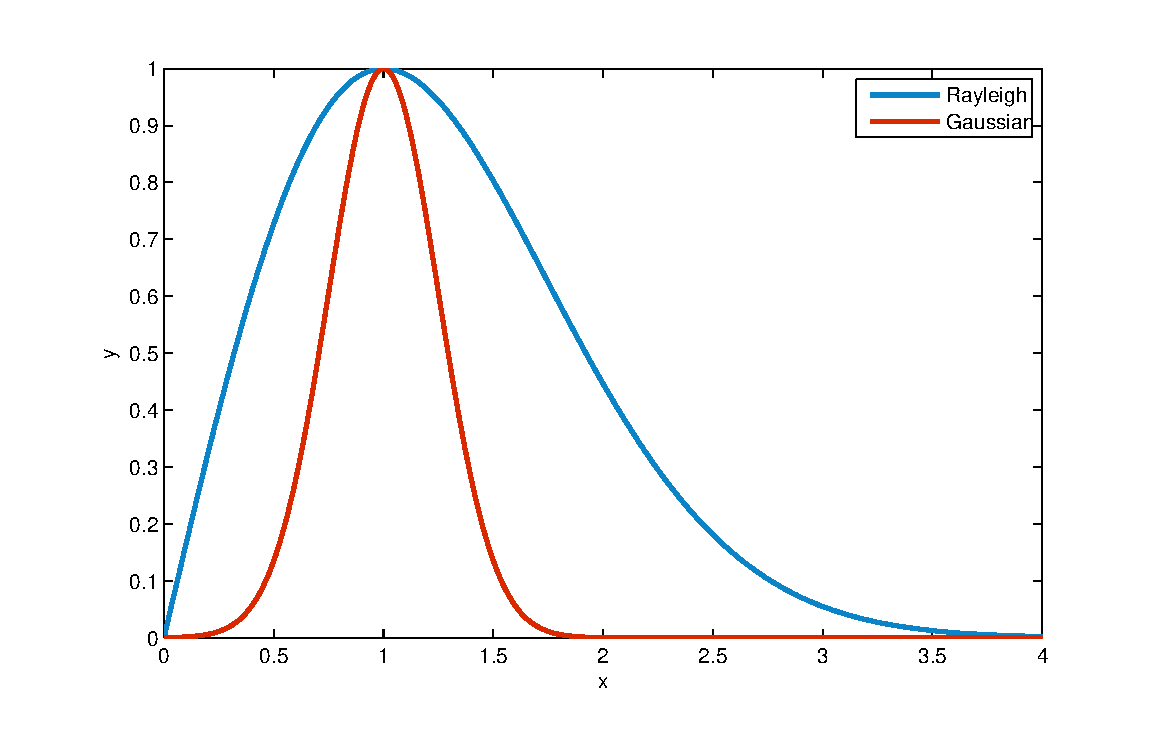
\includegraphics[width=0.7\linewidth]{3_review/figures/processing/pre-processing/noise/noisedistr.eps}
	\caption[Illustration of a Gaussian and Rayleigh distributions.]{Illustration of a Gaussian distribution ($\mu = 1, \sigma=0.25$) and a Rayleigh distribution ( $\sigma = 2$). It can be seen that the Rayleigh distribution is suffering of a bias term when compared with the Gaussian distribution.}
	\label{fig:noisedistr}
\end{figure}

%Noise filtering
%\item[$-$] \textbf{\textit{Noise filtering:}} 
\paragraph{Noise filtering:} The \ac{nmr} signal measured and recorded in the k-space during an \ac{mri} acquisition is affected by noise.
This noise obeys a complex Gaussian white noise mainly due to thermal noises in the patient area \cite{Nowak1999}.
Furthermore, \ac{mri} images visualized by radiologists are in fact the magnitude images resulting from the complex Fourier transform of the k-space data.
The complex Fourier transform, being a linear and orthogonal transform, does not affect the Gaussian noise characteristics \cite{Nowak1999}.
However, the function involved in the magnitude computation is a non-linear transform (i.e., the square root of the sum of squares of real and the imaginary parts), implying that the noise distribution is no longer Gaussian; it indeed follows a Rician distribution making the denoising task harder.
Briefly, a Rician distribution can be characterized as follows: in low-\ac{si} region (low \ac{snr}), it can be approximated with a Rayleigh distribution while in high-\ac{si} region (high \ac{snr}), it is similar to a Gaussian distribution (see Fig. \ref{fig:noisedistr}) \cite{Manjon2008}.
Reviews of all denoising methods can be found in \cite{Buades2005,Mohan2014}.

Median filtering is the simplest approach used to address the denoising issue in \ac{mri} images \cite{Ozer2009,Ozer2010}.
In both studies, Ozer \textit{et al.} used a square kernel of size $5 \times 5$ pixels with the image resolutions ranging from $320 \times 256$ (cf., \ac{t2w} \ac{mri}) to $256 \times 128$ (cf., T$_2$ map, \ac{dce} and \ac{dw} \ac{mri}) and \iac{fov} ranging from 14 cm (cf, \ac{t2w} and \ac{dw} \ac{mri}) to 20 cm (cf, T$_2$ map and \ac{dce} \ac{mri}).
However, from a theoretical point of view, this simple filtering method is not well formalized to address the noise distribution in \ac{mri} images.

More complex approaches were proposed to overcome this problem.
A common method used to denoise \ac{mri} images is based on wavelet-based filtering.
This filtering exploits the sparsity property of the wavelet decomposition.
The projection of a noisy signal from the spatial-domain to the wavelet-domain implies that only few wavelet coefficients contribute to the ``signal-free noise'' while all wavelet coefficients contribute to the noise \cite{Donoho1994}.
Therefore, denoising is performed by thresholding/attenuating the insignificant wavelet coefficients to enforce the sparsity in the wavelet-domain.
Investigations focus on the strategies to perform the most adequate coefficient shrinkage method (e.g., using thresholding, singularity property or Bayesian framework) \cite{Pizurica2002}.

Ampeliotis \textit{et al.} in \cite{Ampeliotis2007,Ampeliotis2008} performed wavelet shrinkage to denoise magnitude \ac{mri} images (cf., \ac{t2w}-\ac{mri} and \ac{dce}-\ac{mri}) using thresholding techniques \cite{Mallat2008}.
However, since the wavelet transform is an orthogonal transform, the Rician distribution of the noise is preserved in the wavelet-domain.
Hence, for low \ac{snr}, the wavelet and scaling coefficients still suffer from a bias due to this specific noise distribution \cite{Nowak1999}.
 
Lopes \textit{et al.} in \cite{Lopes2011} used the filtering technique proposed by \cite{Pizurica2003} to denoise \ac{t2w}-\ac{mri} which was based on joint detection and estimation theory \cite{Pizurica2003}.
{\color{blue}
%Pizurica \textit{et al.} proposed a filtering technique based on joint detection and estimation theory \cite{Middleton1968}.
In this approach, the wavelet coefficients ``free-of-noise'' are estimated from the noisy wavelet coefficients using a \ac{map} estimate.
Furthermore, the estimator designed takes spatial context into account by including both local and global information in the prior probabilities.
The different probabilities needed by the \ac{map} are empirically estimated by using mask images representing the locations of the significant wavelet coefficients.
These mask images are computed by thresholding the detail images obtained from the wavelet decomposition.
To remove the bias from the wavelet and scaling coefficients, the squared magnitude \ac{mri} image used instead of the magnitude \ac{mri} image as proposed by \cite{Nowak1999}.
This involves changing the Rician distribution to a scaled non-central Chi-square distribution.
It implies that the wavelet coefficients are also unbiased estimators and the scaling coefficients are unbiased estimators but up to a constant $C$ as defined in Eq. \eqref{eq:nowakC} which needs to be subtracted from each scaling coefficient,

\begin{equation}
	C=2^{(J+1)}\hat{\sigma}^2 \ ,
	\label{eq:nowakC}
\end{equation}

\noindent where $J$ is the number of levels of the wavelet decomposition and $\hat{\sigma}$ is an estimate of the noise standard deviation.
}
\begin{figure}
\centering
	\includegraphics[width=0.3\linewidth]{3_review/figures/processing/pre-processing/bias/t2w_bias_antenna.eps}
	\caption[Inhomogeneity artefacts due to perturbation of the endorectal coil.]{Example of artefacts with high \ac{si} due to perturbation from the endorectal coil which create inhomogeneity.}
	\label{fig:bias}
\end{figure}


% Artefacts filtering
%\item[$-$] \textbf{\textit{Bias correction:}} 
\paragraph{Bias correction:} Besides being corrupted by noise, \ac{mri} images are also affected by the inhomogeneity of the \ac{mri} field commonly referred to as bias field \cite{Styner2000}.
This bias field results in a smooth variation of the \ac{si} through the image.
When an endorectal coil is used, an artefact resulting of an hyper-intense signal can be observed around the coil on the images (see Fig.~\ref{fig:bias}).

As a consequence, the \ac{si} of identical tissues varies depending on their spatial location in the image making further processes such as segmentation or registration harder \cite{Jungke1987,Vovk2007}.
A review of bias correction methods can be found in \cite{Vovk2007}.

{\color{blue}
The model of image formation is usually formalized such that:

\begin{equation}
	s(\mathbf{x}) = o(\mathbf{x})b(\mathbf{x}) + \eta(\mathbf{x}) \ ,
	\label{eq:biasmodel}
\end{equation}

\noindent where $s(\mathbf{x})$ is the corrupted \ac{si} at the pixel for the image coordinates $\mathbf{x} = \{x,y\}$, $o(\mathbf{x})$ is the ``noise-free signal'' , $b(\mathbf{x})$ is the bias field function and $\eta(\mathbf{x})$ is an additive white Gaussian noise.
%
%By using property of logarithm, the model of Eq. \eqref{eq:biasmodel} becomes additive such that:
%
%\begin{eqnarray}
%	\log s(\mathbf{x}) - \log b(\mathbf{x}) & = & \log \left( o(\mathbf{x}) + \frac{\eta(\mathbf{x})}{b(\mathbf{x})} \right) \ , \\ \nonumber
%	& = & \log \hat{o}(x) \ .
%\end{eqnarray}
%
%\noindent where $\hat{o}(\mathbf{x})$ is the signal only degraded by noise \cite{Styner2000}.

Hence, the task of bias correction involves estimating the bias function $b(\mathbf{x})$ in order to infer the ``signal-free bias'' $o(\mathbf{x})$.
% and subtract to the logarithm of the initial signal in order to obtain an estimated ``signal-free bias''.
}

Viswanath \textit{et al.}~\cite{Viswanath2009} performed bias correction on \ac{t2w}-\ac{mri} using a parametric Legendre polynomial model proposed in \cite{Styner2000} and available in the \ac{itk} library\footnote{The \ac{itk} library is available at: \texttt{http://www.itk.org/}}.

{\color{blue}
Styner \textit{et al.}~\cite{Styner2000} chose to model the bias field by using a linear combination of Legendre polynomials as:

\begin{equation}
	\hat{b}(\mathbf{x},\mathbf{p}) = \sum_{i=0}^{m-1} p_i f_i(\mathbf{x}) =  \sum_{i=0}^{l} \sum_{j=0}^{l-i} p_{ij} P_i(x) P_j(y) \ ,
	\label{eq:biascorr}
\end{equation}

\noindent where $\hat{b}$ is the bias estimation with the image coordinates $\mathbf{x} = \{x,y\}$ and the $m$ coefficients of the linear combination $\mathbf{p} = {p_{11},\dotsc,p_{ij}}$ ; $m$ can be defined as $m=(l+1)\frac{(l+2)}{2}$ where $l$ is the degree of Legendre polynomials chosen and $P_i(\cdot)$ denotes a Legendre polynomial of degree $i$.

This family of functions allows us to model the bias as a smooth inhomogeneity function across the image.
To estimate the set of parameters $\mathbf{p}$, a cost function is defined which relies on the following assumptions: (i) an image is composed of $k$ regions with $\mu_k$ being the mean \ac{si} and a variance $\sigma^{2}_{k}$ of each particular class, and (ii) each noisy pixel belongs to one of the $k$ regions with its \ac{si} value close to the class mean $\mu_k$.
Hence, the cost function is defined as:

\begin{equation}
	C(\mathbf{p}) = \sum_{\mathbf{x}} \prod_{k} \rho_k(s(\mathbf{x}) - \hat{b}(\mathbf{x},\mathbf{p}) - \mu_k) \ ,
	\label{eq:costbias}
\end{equation}

\begin{equation}
	\rho_k(x) = \frac{x^2}{x^2 + 3 \sigma_k^2} \ ,
	\label{eq:mestbias}
\end{equation}

\noindent where $\rho_k(\cdot)$ is a M-estimator allowing estimations to be less sensitive to outliers than usual square distance \cite{Li1996}.

Finally, estimation of the parameters $\mathbf{p}$ results in finding the minimum of the cost function $C(\mathbf{p})$.
This optimization was performed using the non-linear $(1+1)$ \ac{es} optimizer \cite{Styner1997}.

In a later publication, \cite{Viswanath2012} make use of the well known N3 algorithm\footnote{The N3 algorithm implementation is available at: \texttt{http://www.bic.mni.mcgill.ca/\allowbreak software/N3/}} to correct \ac{t2w}-\ac{mri} developed by \cite{Sled1998}.
To estimate the bias function, \cite{Sled1998} proposed to estimate the \acp{pdf} of the signal and bias.

Recalling Eq.~\eqref{eq:biasmodel} and taking advantage of logarithm property, it implies that this model becomes additive such that:

\begin{eqnarray}
	\log s(\mathbf{x}) & = & \log b(\mathbf{x}) + \log \left( o(\mathbf{x}) + \frac{\eta(\mathbf{x})}{b(\mathbf{x})} \right) \ , \nonumber \\
	& \approx & \log b(\mathbf{x}) + \log \hat{o}(\mathbf{x}) \ , \label{eq:logbias}
\end{eqnarray}

\noindent where $\hat{o}(\mathbf{x})$ is the signal only degraded by noise. \cite{Sled1998} shows that Eq. \eqref{eq:logbias} can be related to \acp{pdf} such that:

\begin{equation}
	S(s) = B(s) * O(s) \ ,
	\label{eq:distrbias} 
\end{equation}

\noindent where $S$, $B$ and $O$ are respectively the probability densities of $s$, $b$ and $o$.

Restoring the corrupted signal $s$ is carried out by finding the multiplicative field $b$ which maximizes the frequency content of the distribution $O$.
Sled \textit{et al.}~\cite{Sled1998} argue that a search through all possible fields $b$ and selection of the one which maximizes the high frequency content of $O$ could be carried out but results in an exhaustive search.
However, they show that the bias field distribution can be assimilated to a near Gaussian distribution.
Using this fact as \textit{a priori}, it is then possible to infer the distribution $O$ using Wiener deconvolution given $B$ and $S$ and later estimate the corresponding smooth field $b$.
}

Lv \textit{et al.}~\cite{Lv2009} corrected the inhomogeneity in \ac{t2w}-\ac{mri} images by using the method proposed in \cite{Madabhushi2006}.
In this method, the \ac{mri} images are corrected iteratively by successively detecting the image foreground via \ac{gscale} and estimating a bias field function based on a second-order polynomial model. 
{\color{blue}
First the background of the \ac{mri} image is eliminated by threholding.
The threshold value is commonly equal to the mean \ac{si} of the considered image.
Then, in the seeded region growing algorithm is applied considering every thresholded pixel as a potential seed.
However, pixels already assigned to a region will not be considered any more as seed.
As in seeded region growing algorithm \cite{Shapiro2001}, two criteria are taken into account to expand the region.
First, the region will grow using a connected-neighbourhood, initially defined by the user.
Then, the homogeneity of \ac{si} is based on a fuzzy membership function taking into account the absolute difference of the \acp{si} of two pixels.
Depending on the membership value (cf., a threshold has to be defined), the pixel considered is merged or not to the region.
Once this segmentation is performed, the largest region $R$ is used as a mask to select pixels of the original image and the mean \ac{si}, $\mu_{R}$, is computed. 
The background variation $b(\mathbf{x})$ is estimated as:

\begin{equation}
	b(\mathbf{x}) = \frac{s(\mathbf{x})}{\mu_{R}}, \ \forall \mathbf{x} \in R \ ,
	\label{eq:backest}
\end{equation}

\noindent where $s(\mathbf{x})$ is the original \ac{mri} image.

Finally, a second order polynomial $\hat{b}_{\Theta}(\mathbf{x})$ is fitted in a least-squares sense (Eq.~\eqref{eq:lsolv}),

\begin{equation}
	\hat{\Theta} = \argmin_{\Theta} | b(\mathbf{x}) - \hat{b}_{\Theta}(\mathbf{x}) |^{2}, \ \forall \mathbf{x} \in R \ .
	\label{eq:lsolv}
\end{equation}

Finally, the whole original \ac{mri} image is corrected by dividing it by the estimated bias field function $\hat{b}_{\Theta}(\mathbf{x})$.
This process is repeated until the number of pixels in the largest region $R$ does not change significantly between two iterations.
}

%SI normalization
%\item[$-$] \textbf{\textit{\Ac{si} normalization/standardization:}}
\paragraph{\Ac{si} normalization/standardization:} As discussed in the later section, segmentation or classification tasks are usually performed by first learning from a training set of patients.
Hence, one can emphasize the desire to perform \ac{mri} examinations with a high repeatability or in other words, one would ensure to obtain similar \ac{mri} images (cf., similar \acp{si}) for patients of the same group (cf., healthy patients \textit{vs.} patients with \ac{cap}), for a similar sequence.

However, it is a known fact that variability between patients occurs during the \ac{mri} examinations even using the same scanner, protocol or sequence parameters \cite{Nyul1999}.
Hence, the aim of normalization or standardization of the \ac{mri} data is to remove the variability between patients and enforce the repeatability of the \ac{mri} examinations.
Approaches used to standardize \ac{mri} images can be either categorized as statistical-based standardization or organ \ac{si}-based standardization. 

Artan \textit{et al.}~\cite{Artan2009,Artan2010} as well as Ozer \textit{et al.}~\cite{Ozer2009,Ozer2010} standardized \ac{t2w}, \ac{dce} and \ac{dw} \ac{mri} images by computing the \textit{standard score} (also called \textit{z-score}) of the pixels of the \ac{pz} as:

\begin{equation}
	I_s(\mathbf{x}) = \frac{ I_r(\mathbf{x}) - \mu_{pz}}{\sigma_{pz}}, \ \forall \mathbf{x} \in \text{PZ} \ ,
	\label{eq:meansta}
\end{equation}

\noindent where $I_s(\mathbf{x})$ is the standardized \ac{si} with the image coordinates $\mathbf{x} = \{x,y\}$, $I_r(\mathbf{x})$ is the raw \ac{si}, $mu_{pz}$ is the mean-\ac{si} of the \ac{pz} and $\sigma_{pz}$ is the \ac{si} standard deviation in the \ac{pz}.
This transformation enforces the image \ac{pdf} to have a zero mean and a unit standard deviation.

In a similar way, Liu \textit{et al.}~\cite{Liu2013} normalized \ac{t2w}-\ac{mri} by making use of the median and interquartile range for all the pixels.

Lv \textit{et al.}~\cite{Lv2009} scaled the \ac{si} of \ac{t2w}-\ac{mri} images using the method proposed in \cite{Nyul2000} based on \ac{pdf} matching.
This approach is based on the assumption that \ac{mri} images from the same sequence should share the same \ac{pdf} appearance.
Hence, one can approach this issue by transforming and matching the \acp{pdf} using some statistical landmarks such as median and different quantiles.
Using a training set, these statistical landmarks are extracted for $N$ training images as for instance for the minimum, the $25^{\text{th}}$ quantile, the median, the $75^{\text{th}}$ quantile and the maximum:

\begin{eqnarray}	
	\Phi_{0} & = & \{ \phi_{0}^{1}, \phi_{0}^{2}, \cdots, \phi_{0}^{N} \} \ , \nonumber \\
	\Phi_{25} & = & \{ \phi_{25}^{1}, \phi_{25}^{2}, \cdots, \phi_{25}^{N} \} \ , \nonumber \\
	\Phi_{50} & = & \{ \phi_{50}^{1}, \phi_{50}^{2}, \cdots, \phi_{50}^{N} \} \ ,  \label{eq:quantileStd} \\
	\Phi_{75} & = & \{ \phi_{75}^{1}, \phi_{75}^{2}, \cdots, \phi_{75}^{N} \} \ , \nonumber \\
	\Phi_{100} & = & \{ \phi_{100}^{1}, \phi_{100}^{2}, \cdots, \phi_{100}^{N} \} \ , \nonumber
\end{eqnarray}

\noindent where $\phi_{n^\text{th}}^{i^{\text{th}}}$ is the $n^{\text{th}}$ quantile of the $i^{\text{th}}$ training image.

\begin{figure}
	\centering
	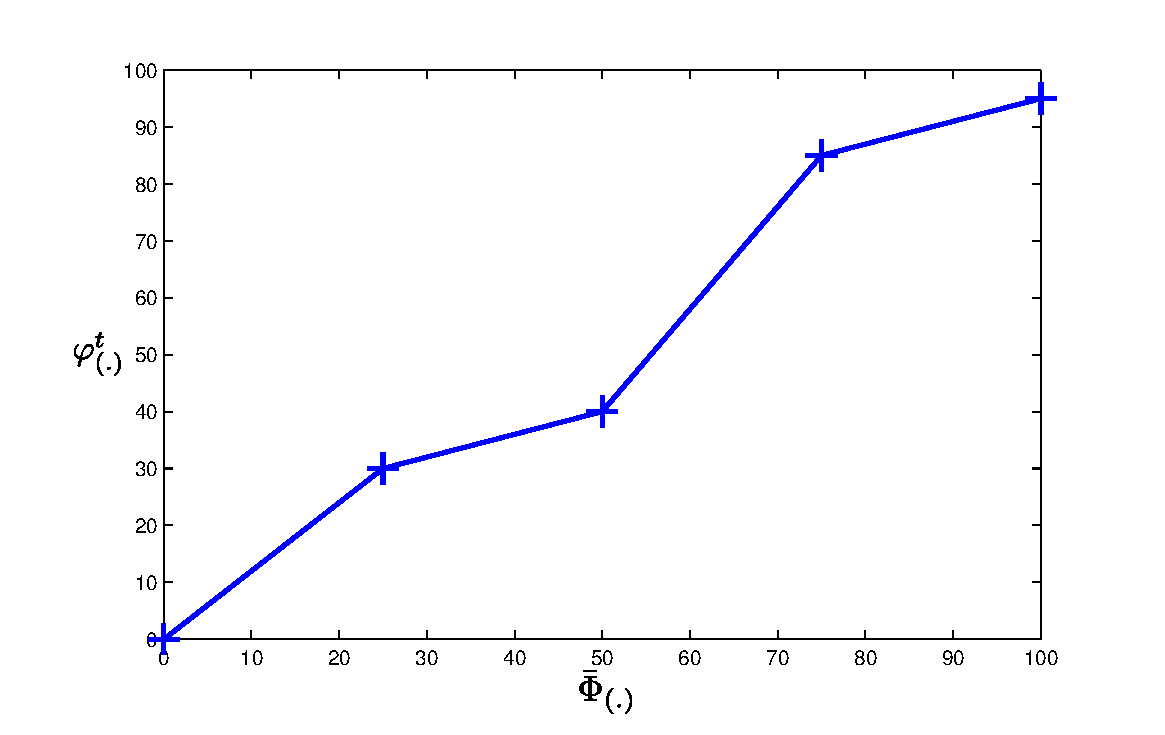
\includegraphics[width=0.7\linewidth]{3_review/figures/processing/pre-processing/normalization/linear_transform_parts.eps}
	\caption{Example of linear mapping by parts as proposed by \cite{Nyul2000}.}
	\label{fig:imnorm}
\end{figure}

Then, the mean of each quantile $\{ \bar{\Phi}_{0}, \bar{\Phi}_{25}, \bar{\Phi}_{50}, \bar{\Phi}_{75}, \bar{\Phi}_{100} \}$ is also calculated.
Once this training stage is performed, a linear transformation by parts $\mathcal{T}(\cdot)$ can be computed (Eq.~\eqref{eq:linearMap}) for each test image $t$ by mapping each statistical landmark $\varphi_{(cdot)}̂^{t}$ of this image with the pre-learned statistical landmarks $\bar{\Phi}_{(\cdot)}$.
This linear mapping is also depicted in Fig.~\ref{fig:imnorm}.

\begin{equation}
\small
\mathcal{T}(s(\mathbf{x})) =
  \begin{cases}
    \lceil \bar{\Phi}_{0}+( s(\mathbf{x}) - \varphi_{0}^{t} ) \left( \frac{\bar{\Phi}_{25} - \bar{\Phi}_{0}}{\varphi_{25}^{t} - \varphi_{0}^{t}} \right) \rceil \ , & \text{if $\varphi_{0}^{t} \leq s(\mathbf{x})<\varphi_{25}^{t})$} \ , \\
    \lceil \bar{\Phi}_{25}+( s(\mathbf{x}) - \varphi_{25}^{t} ) \left( \frac{\bar{\Phi}_{50} - \bar{\Phi}_{25}}{\varphi_{50}^{t} - \varphi_{25}^{t}} \right) \rceil \ , & \text{if $\varphi_{25}^{t} \leq s(\mathbf{x})<\varphi_{50}^{t})$} \ , \\
    \lceil \bar{\Phi}_{50}+( s(\mathbf{x}) - \varphi_{50}^{t} ) \left( \frac{\bar{\Phi}_{75} - \bar{\Phi}_{50}}{\varphi_{75}^{t} - \varphi_{50}^{t}} \right) \rceil \ , & \text{if $\varphi_{50}^{t} \leq s(\mathbf{x})<\varphi_{75}^{t})$} \ , \\
    \lceil \bar{\Phi}_{75}+( s(\mathbf{x}) - \varphi_{75}^{t} ) \left( \frac{\bar{\Phi}_{100} - \bar{\Phi}_{75}}{\varphi_{100}^{t} - \varphi_{75}^{t}} \right) \rceil \ , & \text{if $\varphi_{75}^{t} \leq s(\mathbf{x})\leq \varphi_{100}^{t})$} \ ,
  \end{cases}
  \label{eq:linearMap}
\end{equation}

Viswanath \textit{et al.}~\cite{Viswanath2009,Viswanath2011,Viswanath2012} use a variant of this previous approach presented in \cite{Madabhushi2006a} aiming to standardize the \ac{t2w}-\ac{mri} images.Instead of computing the \ac{pdf} of an entire image, a pre-segmentation of the foreground is carried out via \ac{gscale} which was discussed in the bias correction section.
Once the foreground is detected, the largest region is extracted and the same process than previously mentioned (see Eq.~\eqref{eq:linearMap}) takes place in order to align \acp{pdf} of the foreground of the \ac{mri} images.

\begin{figure}
\centering
	\hspace*{\fill}
	\subfigure[Illustration and location of the bladder on a \ac{t2w}-\ac{mri} image acquired with a 3.0 Tesla \ac{mri} scanner]{\label{subfig:bladder} \includegraphics[width=0.3\linewidth]{3_review/figures/processing/pre-processing/niaf/t2w_bladder.eps}} \hfill
	\subfigure[Illustration and location of the femoral arteries on a \ac{t1w}-\ac{mri} image acquired with a 3.0 Tesla \ac{mri} scanner]{\label{subfig:arteries} \includegraphics[width=0.3\linewidth]{3_review/figures/processing/pre-processing/niaf/t1w_arteries.eps}}
	\hspace*{\fill}
	\caption{Illustration of the two organs used by \cite{Niaf2011,Niaf2012} to normalize \ac{t2w} and \ac{t1w} \ac{mri} images.}
	\label{fig:niaf}
\end{figure}

The methods described above were statistical-based methods.
However, the standardization problem can be tackled by normalizing the MRI images using the \ac{si} of some known organs present in these images. 
Niaf \textit{et al.}~\cite{Niaf2011,Niaf2012} normalized \ac{t2w}-\ac{mri} images by dividing the original \ac{si} of the images by the mean \ac{si} of the bladder (see Fig.~\ref{subfig:bladder}).
Likewise, \cite{Niaf2011} standardized the \ac{t1w}-\ac{mri} images using the \ac{aif}.
They computed the \ac{aif} by taking the mean of the \ac{si} in the most enhanced part of the common femoral arteries (see Fig. \ref{subfig:arteries}) as proposed in \cite{Wiart2007}.

%\end{enumerate}


Presented in Sect.~\ref{subsec:chp2:imaging:mrsi}, \ac{mrsi} is a modality related to a one dimensional signal.
Hence, specific pre-processing steps for this type of signals have been applied instead of standard signal processing methods.

%% \setenumerate{listparindent=\parindent,itemsep=10px}
%% \setlist{noitemsep}
%% \begin{enumerate}[leftmargin=*]

\begin{figure}
	\centering
	\includegraphics[width=0.7\linewidth]{3_review/figures/processing/pre-processing/phase/phase.eps}
	\caption[Illustration of phase malignant in an \ac{mrsi} spectra.]{Illustration of phase misalignment in an \ac{mrsi} spectra acquire with a 3.0 Tesla \ac{mrsi} scanner. Note the distortion of the signal specially visible for the water and citrate peaks.}
	\label{fig:phase}
\end{figure}

%\item[$-$] \textbf{\textit{Phase correction:}}
\paragraph{Phase correction:} \ac{mrsi} data acquired suffer from zero-order and first-order phase misalignments as shown in Fig.~\ref{fig:phase} \cite{Chen2002,Osorio-Garcia2012}. 
Parfait \textit{et al.}~\cite{Parfait2012} used a method proposed in \cite{Chen2002} where the phase of \ac{mrsi} signal is corrected based on entropy minimization in the frequency domain.
The corrected \ac{mrsi} signal $o(\xi)$ can be expressed as:

\begin{eqnarray}
	\Re(o(\xi)) & = & \Re(s(\xi))\cos(\Phi(\xi)) - \Im(\xi)\sin(\Phi(\xi)) \ , \nonumber  \\
	\Im(o(\xi)) & = & \Im(s(\xi))\cos(\Phi(\xi)) + \Re(\xi)\sin(\Phi(\xi)) \ , \nonumber \\
	\Phi(\xi) & = & \phi_0 + \phi_1 \frac{\xi}{N} \ , \label{eq:mrsiphcorr}
\end{eqnarray}

\noindent where $\Re(\cdot)$ and $\Im(\cdot)$ are the real and imaginary part of the complex signal respectively, $s(\xi)$ is the corrupted \ac{mrsi} signal, $\phi_0$ and $\phi_1$ are the zero-order and first-order phase correction terms respectively and $N$ is the total number of samples of the \ac{mrsi} signal.

Chen \textit{et al.}~\cite{Chen2002} tackled this problem using an optimization framework where $\phi_0$ and $\phi_1$ had to be inferred.
Hence, the simplex Nelder-Mead optimization method was used to minimize the following cost function based on the \textit{Shannon entropy} formulation:

\begin{equation}
	\hat{\Phi} = \argmin_{\Phi} \left[ - \sum \Re(s'(\xi)) \ln \Re(s'(\xi)) + \lambda \|\Re(s(\xi))\|_2 \right] \ ,
	\label{eq:phcost}
\end{equation}

\noindent where $s'(\xi)$ is the first derivative of the corrupted signal $s(\xi)$ and $\lambda$ is a regularization parameter.
Once the best parameter $\Phi$ is obtained, the \ac{mrsi} signal is corrected using Eq.~\eqref{eq:mrsiphcorr}.

\begin{figure}
\centering
	\includegraphics[width=0.7\linewidth]{3_review/figures/processing/pre-processing/water/water_fat.eps}
	\caption[Illustration of water and fat residues in \ac{mrsi} signal after supression during acquisition.]{Illustration of the residues of water and fat even after their suppression during the acquisition protocol. The acquisition was carried out with a 3.0 Tesla \ac{mri}.}
	\label{fig:waterfat}
\end{figure}

%\item[$-$] \textbf{\textit{Water and lipid residuals filtering:}} 
\paragraph{Water and lipid residuals filtering:} The water and lipid metabolites occur in much higher concentrations the metabolites of interests (cf., choline, creatine and citrate) \cite{Zhu2010,Osorio-Garcia2012}.
Fortunately, specific \ac{mrsi} sequences were developed in order to suppress water and lipid metabolites using pre-saturation techniques \cite{Zhu2010}.
However, these techniques do not perfectly remove water and lipids peaks and some residuals are still present in the \ac{mrsi} spectra as shown in Fig.~\ref{fig:waterfat}.
Therefore, different post-processing methods have been proposed to enhance the quality of the \ac{mrsi} spectra by removing these residuals.
For instance, Kelm \textit{et al.}~\cite{Kelm2007} used the well known HSVD algorithm proposed by \cite{Pijnappel1992} which models the \ac{mrsi} signal by a sum of exponentially damped sinusoids in the time domain (see Eq.~\eqref{eq:fidsig}).
%In the time domain, a \ac{mrsi} signal $s(t)$ is modelled by a sum of $K$ exponentially damped sinusoids such that:

\begin{equation}
	s(t) = \sum_{k=1}^{K} a_{k}\exp(i \phi_k) \exp( -d_{k} + i 2 \pi f_{k} ) t + \eta(t) \ ,
	\label{eq:fidsig}
\end{equation}

\noindent where $a_k$ is the amplitude proportional to the metabolite concentration with a resonance frequency $f_{k}$, $d_k$ represents the damping factor of the exponential, $\phi_k$ is the first-order phase and $\eta(t)$ is a complex white noise. 

Pijnappel \textit{et al.}~\cite{Pijnappel1992} showed that the ``noise-free signal'' can be found using the \ac{svd} decomposition.
First the noisy signal is reorganized inside a Hankel matrix $H$.
It can be shown that if the signal considered would be a ``noise-free signal'', the rank of $H$ would be equal to rank $K$.
However, due to the presence of noise, $H$ is in fact a full rank matrix.
Thus, to recover the ``noise-free signal'', the rank of $H$ can be truncated to $K$ using its \ac{svd} decomposition.
Hence, knowing the cut off frequencies of water (cf., 4.7 ppm) and lipid (cf., 2.2 ppm) metabolites, their corresponding peaks can be reconstructed and subtracted from the original signal \cite{Laudadio2002}.
	
%\item[$-$] \textbf{\textit{Baseline correction:}} 
\paragraph{Baseline correction:} Sometimes, the problem discussed in the above section regarding the lipid molecules is not addressed simultaneously with water residuals suppression.
Lipids and macromolecules are known to affect the baseline of the \ac{mrsi} spectra.
They could cause errors during further fitting processes aiming to quantify the metabolites, especially regarding the citrate metabolite.
	
Parfait \textit{et al.}~\cite{Parfait2012} made the comparison of two different methods to detect the baseline and correct the \ac{mrsi} spectra which are based on \cite{Lieber2003,Devos2004}. 
Lieber \textit{et al.}~\cite{Lieber2003} addressed the problem of baseline detection in the frequency domain by fitting a low degree  polynomial whereas Parfait \textit{et al.}~\cite{Parfait2012} modified this algorithm by convolvinga Gaussian kernel to smooth the \ac{mrsi} signal instead of fitting a polynomial function.
{\color{red} \textbf{Check the tex file to see the commented area pre-processing.tex}}
%% of low degree $p(x)$ (e.g., second or third degree) to the \ac{mrsi} signal $s(x)$ in a least-squares sense.
%% Then, the values of the fitted polynomial are re-assigned as:

%% \begin{equation}
%% 	p_f(x) = 
%% 	\begin{cases}
%% 		p(x) \ , & \text{if $p(x) \leq s(x)$} \ , \\
%% 		s(x) \ , & \text{if $p(x) > s(x)$} \ . \\
%% 	\end{cases}
%% 	\label{eq:lieber}
%% \end{equation}

%% Finally, this procedure of fitting and re-assignment is iteratively repeated on $p_f(x)$ until a stopping criterion is reached. The final polynomial function can be subtracted from the original signal s(x) to correct it.

%% \cite{Parfait2012} modified this algorithm by convolving a Gaussian kernel to smooth the \ac{mrsi} signal instead of fitting a polynomial function, keeping the rest of the algorithm identical. 
Unlike in \cite{Lieber2003}, Devos \textit{et al.}~\cite{Devos2004} proposed to correct the baseline in the time domain by multiplying the \ac{mrsi} signal by a decreasing exponential function as:
\begin{equation}
	c(t) = \exp (- \beta t) \ ,
	\label{eq:devos}
\end{equation}

\noindent Having a typical value for $\beta$ of 0.15.
However, Parfait \textit{et al.}~\cite{Parfait2012} concluded that the method proposed in \cite{Lieber2003} outperformed the one in \cite{Devos2004}.

In the contemporary work of Tiwari \textit{et al.}~\cite{Tiwari2012}, the authors detected the baseline using a local non-linear fitting method avoiding regions with significant peaks which were detected using a experimentally parametrised signal-to-noise ratio (i.e. a value larger than 5 dB).


\begin{figure}
\centering
	\includegraphics[width=0.7\linewidth]{3_review/figures/processing/pre-processing/frequency/frequency.eps}
	\caption[Illustration of frequency misalignment in an \ac{mrsi} spectra.]{Illustration of frequency misalignment in an \ac{mrsi} spectra acquired with a 3.0 Tesla \ac{mrsi} scanner. The water peak is known to be aligned at 4.65 ppm. However, it can be seen that the peak on this spectra is aligned at around 5.1 ppm.}
	\label{fig:frequency}
\end{figure}

%\item[$-$] \textbf{\textit{Frequency alignment:}} 
\paragraph{Frequency alignment:}
Due to variations of the experimental conditions, a frequency shift can be observed in the \ac{mrsi} spectra \cite{Chen2002,Osorio-Garcia2012} as shown in Fig.~\ref{fig:frequency}.
	
Tiwari \textit{et al.}~\cite{Tiwari2012} corrected the frequency shift by first detecting known metabolite peaks such as choline, creatine and citrate.
The frequency shift is corrected by minimizing the frequency error between the experimental and theoretical values of each of these peaks.

%\item[$-$] \textbf{\textit{Normalization:}} 
\paragraph{Normalization:}
Due to variations of the experimental conditions, the \ac{mrsi} signal may also vary between patients.
Parfait \textit{et al.}~\cite{Parfait2012} as in \cite{Devos2004} compared two methods to normalize \ac{mrsi} signal.
In each method, the original \ac{mrsi} spectra is divided by a normalization factor, similar to the intensity normalization described earlier.  
The first approach to obtain the normalization factor is based on an estimation of the water concentration.
It is required to have an additional \ac{mrsi} sequence where the water metabolites are unsuppressed.
Using this sequence, an estimation of the water concentration can be performed using the previously reported HSVD algorithm.
The second approach to normalization is based on using the L$_2$ norm of the \ac{mrsi} spectra $\|s(\xi)\|_2$. 
It should be noted that both \cite{Parfait2012} and \cite{Devos2004} concluded that the L$_2$ normalization was more efficient in their framework.
 
%\end{enumerate}




\begin{table}
  \caption{Overview of the pre-processing methods used in \ac{cad} systems.}
  \small
  \renewcommand{\arraystretch}{1}
  \begin{tabular}{p{.65\linewidth} p{.25\linewidth}}
    \hline \\ [-1.5ex]
    \textbf{Pre-processing operations} & \textbf{References} \\ \\ [-1.5ex]
    \hline \\ [-1.5ex]
    \textit{\ac{mri} pre-processing:} & \\ \\ [-1.5ex]
    \quad Noise filtering: &  \\
    \quad \quad Median filtering & \cite{Ozer2009,Ozer2010}  \\
    \quad \quad Wavelet-based filtering & \cite{Ampeliotis2007,Ampeliotis2008,Lopes2011} \\ \\ [-1.5ex]
    \quad Bias correction: & \\
    \quad \quad Parametric methods & \cite{Lv2009,Viswanath2009} \\
    \quad \quad Non-parametric methods & \cite{Viswanath2011} \\ \\ [-1.5ex]
    \quad Standardization: & \\
    \quad \quad Statistical-based normalization: & \cite{Artan2009,Artan2010,Lv2009,Ozer2009,Ozer2010,Viswanath2009,Viswanath2011,Viswanath2012} \\
    \quad \quad Organ \ac{si}-based normalization & \cite{Niaf2011,Niaf2012} \\ \\ [-1.5ex]
    \textit{\ac{mrsi} pre-processing:} & \\ \\ [-1.5ex]
    \quad Phase correction & \cite{Parfait2012} \\
    \quad Water and lipid residuals filtering & \cite{Kelm2007} \\
    \quad Baseline correction & \cite{Parfait2012,Tiwari2012} \\
    \quad Frequency alignment & \cite{Tiwari2012} \\
    \quad Normalization & \cite{Parfait2012} \\ \\ [-1.5ex]
    \hline
  \end{tabular}
\label{tab:summary-preproc}
\end{table}

\subsubsection{Segmentation}\label{subsubsec:chp3:lit-clas:img-reg:seg}
The segmentation task consists of delineating the prostate boundaries in the \ac{mri} and is of particular importance for focusing the posterior processing on the organ of interest \cite{Ghose2012}. 
In this section, only the segmentation methods used in \ac{cad} for \ac{cap} are presented and summarized in Table.~\ref{tab:summary-seg}.
These methods are mostly intensity based.
 An exhaustive review of prostate segmentation methods in \ac{mri} can be found in \cite{Ghose2012}.

\begin{table}
	\caption{Overview of the segmentation methods used in \ac{cad} systems.}
	\small
	%\renewcommand{\arraystretch}{1.5}
	\begin{tabular}{p{.65\linewidth} p{.25\linewidth}}
		\hline \\ [-1.5ex]
		\textbf{Segmentation methods} & \textbf{References} \\ \\ [-1.5ex]
		\hline \\ [-1.5ex]
		\textit{\ac{mri}-based segmentation:} & \\ \\ [-1.5ex]
		\quad Manual segmentation & $[$4-5,16,18-21,24,38-40$]$ \\
		\quad Region-based segmentation & $[$11$]$ \\
		\quad Hybrid segmentation & $[$10,34-36,41$]$ \\ \\ [-1.5ex]
		\textit{\ac{mrsi}-based segmentation:} & \\ \\ [-1.5ex]
		\quad Clustering & $[$28$]$ \\ \\ [-1.5ex]
		\hline
	\end{tabular}
\label{tab:summary-seg}
\end{table}

\setenumerate{listparindent=\parindent,itemsep=10px}
\setlist{noitemsep}
\begin{enumerate}[leftmargin=*]

\item[$-$] \textbf{\textit{Manual segmentation:}} To highlight the importance of prostate segmentation task in \ac{cad} systems, it is interesting to note the large number of studies which manually segment the prostate organs \cite{Artan2009,Artan2010,Matulewicz2013,Niaf2011,Niaf2012,Ozer2009,Ozer2010,Puech2009,Vos2008,Vos2008a}.
In all the cases, the boundaries of the prostate gland are manually defined in order to limit further processing to only this area.
This approach ensures the right delineation of the organ nevertheless this procedure is highly time consuming and should be performed by a radiologist.

\item[$-$] \textbf{\textit{Region-based segmentation:}} Litjens \textit{et al.} in \cite{Litjens2012} used a multi-atlas-based segmentation using multi-modal images (e.g., \ac{t2w}-\ac{mri} and \ac{adc} map) to segment the prostate with an additional pattern recognition method to differentiate \ac{cg} and \ac{pz} as proposed in \cite{Litjens2012a}.
This method consists in three different steps: (i) the registration between each atlas and the multi-modal images, (ii) the atlas selection and finally (iii) the classification of the prostate segmented voxels in either \ac{cg} or \ac{pz}. 
The registration between each atlas and the \ac{mri} images is performed using two successive registrations; the first registration is a rigid registration to roughly aligned the atlases and the \ac{mri} images and the second is an elastic registration using B-spline transformation.
The objective function to perform the registration is defined as the weighted sum of the metric of both \ac{t2w}-\ac{mri} and \ac{adc} map.
The metric is based on \ac{mi} (please refer to the next section for more details in regard to registration).
Two strategies of atlas selection were performed by using either a majority voting approach or the \ac{staple} approach \cite{Warfield2004}.
After segmentation of the prostate, the differentiation of both \ac{cg} and \ac{pz} has to be carried out.
This problem was carried out by classifying each voxel using \ac{lda}.
Three types of features were considered: (i) anatomy, (ii) intensity and (iii) texture.
Regarding the anatomy, relative position and relative distance from the pixel to the border of the prostate were used.
The intensity features consist in the intensity of the voxel in the ADC coefficient and the T$_2$ map.
The texture features were composed of five different features: homogeneity, correlation \cite{Amadasun1989}, entropy, texture strength \cite{Li2005a} and \ac{lbp} \cite{Ojala1996}.
Finally, some morphological operations were applied to remove artefact and the contour between the zones were smooth using the \ac{tps} \cite{Bookstein1989}.

Litjens \textit{et al.} in \cite{Litjens2014} used an almost identical algorithm proposed by PROMISE12 challange \cite{Litjens2014a}.
Their segmentation method is also based on multi-atlas multi-modal images, but the SIMPLE method \cite{langerak2010label} is used instead to combine labels after the registration of the different atlas to obtain the final segmentation.
 
\item[$-$] \textbf{\textit{Hybrid-based segmentation:}} Viswanath \textit{et al.} in \cite{Viswanath2008a,Viswanath2009} used a \ac{mantra} method as proposed in \cite{Toth2008}.
\ac{mantra} is closely related to the \ac{asm} from \cite{Cootes1995}.
This algorithm consists of two stages: (i) a training stage where a shape and appearance model is generated and (ii) the actual segmentation performed based on the learned model. 
For the training stage, a set of landmarks is defined and the shape model is generated as in the original \ac{asm} method \cite{Cootes1995}.
{\color{red}\textbf{Check what is commented in the segmentation.tex here, it was not explained well so I didnt included them.}}

%% Then, to model the appearance, a set of $K$ texture images $\{I_1,I_2,\cdots,I_k\}$ based on first and second order statistical texture features, are computed.
%% For a given landmark $l$ with its given neighbourhood $\mathcal{N}(l)$, its feature matrix extracted can be expressed as:

%% \begin{equation}
%% 	f_l = \{ I_1(\mathcal{N}(l)), I_2(\mathcal{N}(l)), \cdots, I_k(\mathcal{N}(l)) \} \ .	
%% 	\label{eq:mantra1}
%% \end{equation}

%% \noindent where $I_k(\mathcal{N}(l))$ represent a feature vector obtained by sampling the $k^{\text{th}}$ texture map using the neighbourhood $\mathcal{N}(l)$.
%% By generating multiple landmark in the same fashion as the \ac{asm}, \ac{pca} \cite{Pearson1901} is applied to learned the appearance variations.
%% For the segmentation stage, the mean shape learned previously is initialise in the test image.
%% The same associated texture images as in the training stage are computed.
%% For each landmark $l$, a neighbourhood of a larger size than $\mathcal{N}(l)$ is defined where multiple neighbourhoods $\mathcal{N}_R(l)$ of same size than $\mathcal{N}(l)$ will be generated.
%% Each $\mathcal{N}_R(l)$ patch will be used to sample the texture images and a reconstruction will be performed using the appearance trained model.
%% The new landmark location will be defined as the position where the \ac{mi} is maximal between the reconstructed and original values.
%% This scheme is performed in a multi-resolution manner as in \cite{Cootes1995}.}

%% \cite{Viswanath2012} used a \ac{weritas} proposed by \cite{Toth2009}. As \ac{mantra} method, this is really close to \ac{asm} formulation. 

%% In the training stage, a set of landmarks $\{l_1,l_2,\cdots,l_n\}$ associated with their given neighbourhood $\{\mathcal{N}(l_1),\mathcal{N}(l_2),\cdots,\mathcal{N}(l_n)\}$ are defined. 

%% In the same way, a set of pixels $\{p_1,p_2,\cdots,p_n\}$ associated with their given neighbourhood $\{\mathcal{N}(p_1),\mathcal{N}(p_2),\cdots,\mathcal{N}(p_n)\}$ are defined. 

%% A set of $K$ texture images $\{I_1,I_2,\cdots,I_k\}$ based on first and second order statistical texture features, are computed from the original image $I_0$. Hence, for a given landmark $l$ with its given neighbourhood $\mathcal{N}(l)$, its feature matrix extracted can be expressed as:

%% \begin{equation}
%% 	f_l = \{ I_1(\mathcal{N}(l)), I_2(\mathcal{N}(l)), \cdots, I_k(\mathcal{N}(l)) \} \ .	
%% 	\label{eq:weritas1}
%% \end{equation}

%% \noindent where $I_k(\mathcal{N}(l))$ represents a feature vector obtained by sampling the $k^{\text{th}}$ texture map using the neighbourhood $\mathcal{N}(l)$.

%% In the same way, for a given pixel $p$ with its given neighbourhood $\mathcal{N}(p)$, its feature matrix extracted can be expressed as:

%% \begin{equation}
%% 	f_p = \{ I_1(\mathcal{N}(p)), I_2(\mathcal{N}(p)), \cdots, I_k(\mathcal{N}(p)) \} \ .	
%% 	\label{eq:weritas2}
%% \end{equation}

%% \noindent where $I_k(\mathcal{N}(p))$ represents a feature vector obtained by sampling the $k^{\text{th}}$ texture map using the neighbourhood $\mathcal{N}(p)$.

%% Also, each of the feature $f_l$ and $f_p$ are associated with their means $\bar{f}_l$ and $\bar{f}_p$ and their covariance $\Phi_l$ and $\Phi_p$. A set of of Euclidean distance is computed for each landmark and pixel such that:

%% \begin{equation}
%% 	E = \{ \| l - p \|_2 \} \ .
%% 	\label{eq:weritas3}
%% \end{equation}

%% A set of Mahalanobis distance will also be computed such that:


Litjens \textit{et al.}~\cite{Litjens2011} and Vos \textit{et al.}~\cite{Vos2012} used an approach proposed in \cite{Huisman2010} in which the bladder, prostate and rectum are segmented.

The segmentation task is performed as an optimization problem taking three parameters into account linked to organs such as: (i) the shape (an ellipse), (ii) the location and (iii) the respective angles between them.
%% First, a probabilistic model is first trained by embedding the three following aspects: (i) the shape by defining each organ as an ellipse, (ii) the position by defining the distance and the angle between each organ center and (iii) the appearance using the \acp{pdf} of \ac{si} of each organ. 
Furthermore, Litjens \textit{et al.}~\cite{Litjens2011} used only \ac{adc} map to encode the appearance whereas Vos \textit{et al.}~\cite{Vos2012} used both \ac{adc} and T$_2$ maps.
%Then, during the optimization using a quasi-Newton optimizer, an objective function is minimized. 
%% This function is defined as the sum of the deviations from the above model learnt. This rough segmentation is then used inside a Bayesian framework to refine the shape. {\color{red}Really have to check because things seem to be made up.}


Only the work of Tiwari \textit{et al.} in \cite{Tiwari2009} propose a segmentation based on \ac{mrsi}.
Authors localized the voxels corresponding to the prostate organ using a hierarchical spectral clustering.
First, each \ac{mrsi} spectrum is projected into a lower dimension space using graph embedding \cite{Shi2000}.
To proceed, a similarity matrix $W$ is computed using a Gaussian similarity measure from Euclidean distance \cite{Belkin2001}) such that:

\begin{equation}
	W(\mathbf{x},\mathbf{y}) =
	\begin{cases}	
	 	\exp \left( \frac{\| s(\mathbf{x}) - s(\mathbf{y}) \|_2^2}{\sigma^2} \right) \ , & \text{if } \| \mathbf{x} - \mathbf{y} \|_2 < \epsilon \ , \\
	 	0 \ , & \text{if } \| \mathbf{x} - \mathbf{y} \|_2 > \epsilon \ .
	 \end{cases}
	\label{eq:ge1}
\end{equation}

\noindent where $s(\mathbf{x})$ and $s(\mathbf{y})$ are the \ac{mrsi} spectra for the voxels $\mathbf{x}$ and $\mathbf{y}$ respectively, $\sigma$ is the standard deviation of the Gaussian similarity measure and $\epsilon$ is the parameter to defined an $\epsilon$-neighbourhood.
The projection can be performed as a generalized eigenvector problem such that:
\begin{eqnarray}
	Lu & = & \lambda D u \ , \nonumber \\
	D(\mathbf{x},\mathbf{x}) & = & \sum_{\mathbf{y}} W(\mathbf{x},\mathbf{y}) \ , \label{eq:ge2} \\
	L & = & D-W \ . \nonumber
\end{eqnarray}

\noindent where $D$ is the diagonal weight matrix, $L$ is the Laplacian matrix, $\lambda$ and $u$ represent the eigenvalues and eigenvectors.
Once that the \ac{mrsi} spectra are projected into the lower dimension space, a replicate k-means clustering method is used to define two clusters where the larger cluster is assimilated to be the cluster corresponding to non-prostate voxels and will be eliminated.
The full procedure is repeated until the total number of voxels left is inferior to a given number.


\end{enumerate}


%% \subsection{Segmentation} \label{subsec:segmentation}

%% The segmentation task consists in delineating the prostate boundaries in the \ac{mri}. This procedure is of particular importance for focusing the posterior processing on the organ of interest (\cite{Ghose2012}). In this section, only the segmentation methods used in \ac{cad} systems are presented and summarized in Tab. \ref{tab:seg}. An exhaustive review of prostate segmentation methods in \ac{mri} can be found in \cite{Ghose2012}.


%% \setenumerate{listparindent=\parindent,itemsep=10px}
%% \setlist{noitemsep}
%% \begin{enumerate}[leftmargin=*]

%% \item[$-$] \textbf{\textit{Manual segmentation:}} To highlight the importance of prostate segmentation task in \ac{cad} systems, it is interesting to note the large number of studies which segment manually the prostate organs (\cite{Artan2009,Artan2010,Matulewicz2013,Niaf2011,Niaf2012,Ozer2009,Ozer2010,Puech2009,Vos2008,Vos2008a}). In all the cases, the boundaries of the prostate gland is defined in order to limit the further processing to only this area. This approach ensure the right delineation of the organ nevertheless this procedure is highly time consuming and should be perform by a radiologist.

%% \item[$-$] \textbf{\textit{Region-based segmentation:}} \cite{Litjens2012} used a multi-atlas-based segmentation using multi-modal images (e.g., \ac{t2w}-\ac{mri} and \ac{adc} map) to segment the prostate with an additional pattern recognition method to differentiate \ac{cg} and \ac{pz} as proposed in \cite{Litjens2012a}. This method consists of three different steps: (i) the registration between each atlas and the multi-modal images, (ii) the atlas selection and finally (iii) the classification of the prostate segmented voxels in either \ac{cg} or \ac{pz}. 

%% The registration between each atlas and the \ac{mri} images is performed using two successive registrations: the first registration is a rigid registration to roughly align the atlases and the \ac{mri} images and the second is an elastic registration using B-spline transformation. The objective function to perform the registration is defined as the weighted sum of the metric of both \ac{t2w}-\ac{mri} and \ac{adc} map. The metric is based on \ac{mi}. We refer to the next section for more details in regard to registration. Two strategies of atlas selection were performed by using either a majority voting approach or the \ac{staple} approach (\cite{Warfield2004}).

%% Subsequently,  \ac{cg} and \ac{pz} segmentation within the prostate region is achieved by classifying each voxel using a \ac{lda} classifier. Three types of features were considered: (i) anatomy, (ii) intensity and (iii) texture. Regarding the anatomy, relative position and relative distance from the pixel to the border of the prostate were used. The intensity features consist of the intensity of the voxel in the ADC coefficient and the T$_2$ map. The texture features were composed of five different features: homogeneity, correlation (\cite{Amadasun1989}), entropy, texture strength (\cite{Li2005a}) and \ac{lbp} (\cite{Ojala1996}). Finally, morphological operations were applied to remove artefacts and the contours between the zones were smoothed using \ac{tps} (\cite{Bookstein1989}).

%% \item[$-$] \textbf{\textit{Model-based segmentation:}} \cite{Viswanath2008a,Viswanath2009} used the \ac{mantra} method as proposed by \cite{Toth2008}. \ac{mantra} is closely related to the \ac{asm} from \cite{Cootes1995}. This algorithm consists of two stages: (i) a training stage where a shape and appearance model is generated and (ii) the actual segmentation performed based on the learned model. 

%% For the training stage, a set of landmarks is defined and the shape model is generated as in the original \ac{asm} method (\cite{Cootes1995}). Then, to model the appearance, a set of $K$ texture images $\{I_1,I_2,\cdots,I_k\}$ based on first and second order statistical texture features are computed. For a given landmark $l$ with its given neighbourhood $\mathcal{N}(l)$, its feature matrix extracted can be expressed as:

%% \begin{equation}
%% 	f_l = \{ I_1(\mathcal{N}(l)), I_2(\mathcal{N}(l)), \cdots, I_k(\mathcal{N}(l)) \} \ ,
%% 	\label{eq:mantra1}
%% \end{equation}

%% \noindent where $I_k(\mathcal{N}(l))$ represents a feature vector obtained by sampling the $k^{\text{th}}$ texture map using the neighbourhood $\mathcal{N}(l)$.

%% By generating multiple landmarks in the same fashion as \ac{asm}, \ac{pca} (\cite{Pearson1901}) is applied to learn the appearance variations.

%% For the segmentation stage, the mean shape learned previously is initialised in the test image. The same associated texture images as in the training stage are computed. For each landmark $l$, a neighbourhood of patches are used to sample the texture images and a reconstruction is obtained using the appearance model previously trained. The new landmark location will be defined as the position where the \ac{mi} is maximal between the reconstructed and original values. This scheme is performed in a multi-resolution manner as in \cite{Cootes1995}.

%% Subsequently, the same authors (\cite{Viswanath2012}) used the \ac{weritas} method also proposed by \cite{Toth2009}. As with the \ac{mantra} method, \ac{weritas} is based on the \ac{asm} formulation. In fact it is very close to the \ac{mantra} itself. The same texture features are used to construct the appearance models, but instead of using \ac{mi} between the landmarks and neighbour patches for adapting the landmark positions, it defines a metric based on the Mahalanobis distance. In the training stage, the Mahalanobis distance is computed between landmarks and neighbour patches for each of the features. Subsequently, a new metric is proposed as a linear weighted combination of those Mahalanobis distances which maximises the correlation with the Euclidean distance between the patches and the true landmarks. In the segmentation step, this metric is then computed between the initialised landmarks and neighbouring patches in order to update landmark positions, in a similar fashion to other \ac{acm} models. 

%% \cite{Litjens2011} and \cite{Vos2012} used an approach proposed by \cite{Huisman2010} in which the bladder, prostate and rectum are segmented tackling the segmentation task as an optimization problem. A probabilistic model is first trained by embedding the three following aspects: (i) the shape by defining each organ as an ellipse, (ii) the position by defining the distance and the angle between each organ center and (iii) the appearance using the \acp{pdf} of \ac{si} of each organ. \cite{Litjens2011} used only \ac{adc} map to encode the appearance whereas \cite{Vos2012} used both \ac{adc} and T$_2$ maps. Then, during the optimization using a quasi-Newton optimizer, an objective function is minimized. This function is defined as the sum of the deviations from the above model learnt. This rough segmentation is then used inside a Bayesian framework to refine the segmentation.

%% \end{enumerate}

%% \subsubsection{MRSI-based segmentation}

%% \cite{Tiwari2009} localized the voxels corresponding to the prostate organ using a hierarchical spectral clustering. First, each \ac{mrsi} spectrum is projected into a lower dimension space using graph embedding (\cite{Shi2000}). To proceed, a similarity matrix $W$ is computed using a Gaussian similarity measure from the Euclidean distance (\cite{Belkin2001}) such that:

%% \begin{equation}
%% 	W(\mathbf{x},\mathbf{y}) =
%% 	\begin{cases}	
%% 	 	\exp \left( \frac{\| s(\mathbf{x}) - s(\mathbf{y}) \|_2^2}{\sigma^2} \right) \ , & \text{if } \| \mathbf{x} - \mathbf{y} \|_2 < \epsilon \ , \\
%% 	 	0 \ , & \text{if } \| \mathbf{x} - \mathbf{y} \|_2 > \epsilon \ ,
%% 	 \end{cases}
%% 	\label{eq:ge1}
%% \end{equation}

%% \noindent where $s(\mathbf{x})$ and $s(\mathbf{y})$ are the \ac{mrsi} spectra for the voxels $\mathbf{x}$ and $\mathbf{y}$ respectively, $\sigma$ is the standard deviation of the Gaussian similarity measure and $\epsilon$ is a parameter used to define an $\epsilon$-neighbourhood.

%% The \ac{mrsi} spectra projection into the lower dimension space is approached as a generalized eigenvector problem. Subsequently, a replicate k-means clustering method is run defining two clusters. The data corresponding to larger cluster is assumed to belong to the non-prostate voxels and these voxels will be eliminated from the processing. The full procedure is repeated until the total number of voxels left is inferior to a given threshold set experimentally.

\subsection{Registration}\label{subsec:chp3img-reg:reg}
\input{3_review/fig-reg-framework.tex}

The role of image registration is vital in \ac{cad} systems using multi-parametric \ac{mri} images. 
As it will be discussed in Sect.~\ref{sec:chp3clas}, for the sake of an optimal classification, the features detected in each modality will be grouped depending of their spatial locations. 
Hence, one has to ensure the perfect alignment of the multi-modal \ac{mri} images ahead of performing any classification.

Image registration is the procedure consisting of aligning an unregistered image (also called moving image) into a template image (also called fixed image) via a geometric transformation.
This problem is usually addressed as presented in Fig.~\ref{fig:frareg}.
An iterative procedure takes place to infer the geometric transformation (parametric or non-parametric) via an optimizer, which maximizes the similarity between the two images.
In the following, a review of the different components of a typical registration framework: transformation model, similarity metric, optimizer and interpolation are presented, followed by a summary of registratio approaches applied in \ac{cad} for \ac{cap} syetems.
Exhaustive reviews covering all registration methods in computer science and medical fields can be found in \cite{Maintz1998} and \cite{Zitova2003}.

%From Sect. \ref{subsubsec:geotra} to \ref{subsubsec:int}, we individually review the different components of a typical registration framework (Fig \ref{fig:frareg}).
%Section \ref{subsubsec:regrev} will summarize the combinations of these components especially for the frameworks used in \ac{cad} systems. 

%% \setenumerate{listparindent=\parindent,itemsep=10px}
%% \setlist{noitemsep}
%% \begin{enumerate}[leftmargin=*]

%\item[$-$] \textbf{\textit{Geometric transformation models:}} 
\paragraph{Geometric transformation models:}
%% From all \ac{cad} for \ac{cap} systems reviewed, only parametric transformation models have been used, mainly based on affine and elastic transformation.
%% Affine transformations provide dgrees of freedom managaing rotations and translation as with the rigid transformations but also shearing and scaling.
As previously mentioned, the registration problem is to align two images or volumes by finding the geometric transformation.
Regarding the transformation, from all \ac{cad} systems reviewed, only parametric methods have been implemented.
Three different groups of parametric transformation models have been used, rigid, affine, and elastic, each of them are characterized by the degree of freedom that they offer.

The first type of transformation is usually referred to as rigid transformation.
These transformations are only composed of rotation and translation transforms.
Hence, for a 2D space where $\mathbf{x} = (x,y) \in \mathbb{R}^2$, a rigid transformation $\mathcal{T}_R$ is formalized as as:

\begin{eqnarray}
	\mathcal{T}_R(\mathbf{x}) & = & \begin{bmatrix}
		R & \mathbf{t} \\
		\mathbf{0^T} & 1
	\end{bmatrix} \mathbf{x} \ , \nonumber \\
	& = & \begin{bmatrix}
		\cos \theta & -\sin \theta & t_x \\
		\sin \theta & \cos \theta & t_y \\
		0 & 0 & 1
	\end{bmatrix}\begin{bmatrix}
		x \\
		y \\
		1
	\end{bmatrix} \ , \label{eq:rigtra} %\\
\end{eqnarray}

\noindent where $\theta$ is the rotation angle and $\{ t_x,t_y \}$ represents the translation along $\{x,y\}$ respectively.

In the case of 3D registration using volume, an additional component $z$ has to be taken into account such that $\mathbf{x} = (x,y,z)$.
Thus, the rotation matrix $\mathbf{R}$ becomes of size $3 \times 3$ whereas the translation vector $\mathbf{t}$ consists of a vector of three elements. 
Hence, the geometric transformation $\mathcal{T}_R(\cdot)$ is embedded into a matrix of size $4 \times 4$.

Affine transformations provide additional degrees of freedom managing rotations and translation as with the rigid transformations but also shearing and scaling.
Hence, for a 2D space where $\mathbf{x} = (x,y) \in \mathbb{R}^2$, an affine transformation $\mathcal{T}_A$ is formalized as: 

\begin{eqnarray}
	\mathcal{T}_A(\mathbf{x}) & = & \begin{bmatrix}
		A & \mathbf{t} \\
		\mathbf{0^T} & 1
	\end{bmatrix} \mathbf{x} \ , \nonumber \\
	& = & \begin{bmatrix}
		a_{11} & a_{12} & t_x \\
		a_{21} & a_{22} & t_y \\
		0 & 0 & 1
	\end{bmatrix}\begin{bmatrix}
		x \\
		y \\
		1
	\end{bmatrix} \ . \label{eq:afftra}% 
\end{eqnarray}
\noindent Hence the four parameters $\{a_{11},a_{12},a_{21},a_{22}\}$ of the affine matrix and $\{ t_x, t_y \}$ of the translation encode an affine transformation.

Regarding volume registeration, the previously mentioned remark can be applied as well.
Thus the geometric transformation $\mathcal{T}_A(\cdot)$ is of size $4 \times 4$ with nine parameters involved.

Finally, the last group of transformations is known as elastic transformations and offer the advantage to handle local distortions.
In the reviewed \ac{cad} systems, the radial basis functions are used to formalize the local distortions such as:

\begin{equation}
	\mathcal{T}_E(\mathbf{x}) = \begin{matrix}
	a_{11} x - a_{12} y + t_x + \sum_i c_i g(\| \mathbf{x} - p_i \|) \\
	a_{21} x + a_{22} y + t_y + \sum_i c_i g(\| \mathbf{x} - p_i \|)
	\end{matrix} \ ,
\end{equation}

\noindent where $\mathbf{x}$ are the control points in both images and $g(\cdots)$ is the actual radial basis function. 

Two radial basis functions are used: (i) the \ac{tps} and (ii) the B-splines.
Apart from the formalism, these two approaches have a main difference: with B-splines, the control points are usually uniformly and densely placed on a grid where as with \ac{tps}, the control points correspond to detected or selected key points.
By using \ac{tps}, Mitra \textit{et al.}~\cite{Mitra2011} obtained more accurate and time efficient results than with the B-splines strategy \cite{Mitra2012a}.

It is reasonable to point out that usually only rigid or affine registrations are used to register multi-parametric images from a same protocol.
Elastic registration methods are more commonly used to register multi-protocol images (e.g., histopathology with \ac{mri} images) \cite{Toth2008,Toth2009}.

%\item[$-$] \textbf{\textit{Similarity measure:}} 
\paragraph{Similarity measure:}
%% During the registration procedure, a similarity criterion is computed in order to evaluate the quality of the alignment performed.
%% Roughly speaking, this criterion will give the direction to take to the optimizer, in order to assign the most optimal values to the geometric transformation parameters.
The most naive similarity measure used in reviewed registration framework is the \acf{mse} of the \ac{si} of \ac{mri} images.
For a pair of images $I$ and $J$, the \ac{mse} is formalized as:

\begin{equation}
	\text{MSE} =\frac{1}{N} \sum_x \sum_y ( I(x,y) - J(x,y) )^2 \ ,
	\label{eq:mse}
\end{equation}
\noindent where $N$ is the total number of pixels.
This metric is not well suited when multi-parametric images are involved due to the tissue appearance variations between the different modalities.

\begin{figure}
\centering
	\hspace*{\fill}
	\subfigure[Illustration of a joint histogram between to aligned image.]{\label{subfig:histoalgn}\includegraphics[width=0.2\textwidth]{3_review/figures/processing/registration/histogram/jointhistoalg.eps}} \hfill
	\subfigure[Illustration of a joint histogram between to misaligned image.]{\label{subfig:histomisalgn} \includegraphics[width=0.2\textwidth]{3_review/figures/processing/registration/histogram/jointhistomisal.eps}}
	\hspace*{\fill}
	\caption[Difference observed in joint histogram between aligned and misaligned images.]{Difference observed in joint histogram between aligned and misaligned images. The joint measure will be more concentrated of the histogram in the case that the images are aligned and more randomly distributed in the case that both images are more misaligned.}
\end{figure}

In that regard, \ac{mi} was introduced as a registration measure in the late 1990's by \cite{Pluim2003}.
The \ac{mi} measure finds its foundation in the assumption that a homogeneous region in the first modality image should also appear as a homogeneous region in the second modality even if their \acp{si} are not identical.
Thus, those regions share information and the registration task can be achieved by maximizing this common information.
Hence, \Ac{mi} of two images $A$ and $B$ is defined as:

\begin{equation}
	MI(A;B) = S(A) + S(B) - S(A,B) \ ,
	\label{eq:midef}
\end{equation}

\noindent where $S(A)$ and $S(B)$ are the marginal entropies and $S(A,B)$ is the joint entropy.
Then, maximizing the \ac{mi} is equivalent to minimizing the joint entropy. 
The joint entropy measure is related with the degree of uncertainty or dispersion of the data in the joint histogram of the images $A$ and $B$.
As shown in Fig.~\ref{fig:jointhisto}, the data in the joint histogram will be concentrated in the case of aligned images while will be more randomly distributed in the case of misaligned images.
Regarding the computation of the entropies, an estimation of the \acp{pdf} have to be carried out.
Histogram or Parzen window methods are a common way to estimate these \acp{pdf}.

A generalized form of \ac{mi}, \ac{cmi}, was proposed by \cite{Chappelow2011}.
\ac{cmi} encompasses interdependent information such as texture and gradient into the metric.
Hence, for both of images $A$ and $B$, the image ensembles $\epsilon^{A}_n$ and $\epsilon^{B}_m$ are generated and composed of $n$ and $m$ images based on the texture and gradient.
Then, the \ac{cmi} can be formulated such as:

\begin{equation}
	CMI(\epsilon^{A}_n;\epsilon^{B}_m) = S(\epsilon^{A}_n) + S(\epsilon^{B}_m) - S(\epsilon^{A}_n,\epsilon^{B}_m) \ .
	\label{eq:cmidef}
\end{equation}

{\color{red} \textbf{Check the commented text, It is not well written and I did not include them}}
%% \noindent From Eq. \eqref{eq:cmidef}, it can be seen that \ac{cmi} is estimated using high dimensional data and that the histogram-based methods to estimate the \acp{pdf} are not suitable any more \cite{Chappelow2011}. 
%% However, other approaches can be used such as the one employed by \cite{Staring2009} to compute the $\alpha$-\ac{mi} \cite{Hero2002}) which is based on the construction of entropic graphs using \ac{knn} inside the high dimensional feature space later used to estimate the \ac{mi}.

%\item[$-$] \textbf{\textit{Optimization methods:}} 
\paragraph{Optimization methods:}
Registration is usually regarded as an optimization problem where the parameters of the geometric transformation model have to be inferred by minimizing the similarity measure.
Iterative estimation methods are commonly used being the L-BFGS-B quasi-Newton method \cite{Byrd1995} and gradient descent \cite{Viola1997} the most common ones. % Nelder-Mead simplex method \cite{Nelder1965},
During our review, we noticed that authors do not usually linger over optimizer choice.

%\item[$-$] \textbf{\textit{Interpolation:}}
\paragraph{Interpolation:} 
The registration procedure involves transforming an image, and pixels mapped to non-integer points must be approximated using interpolation methods.
As for the optimization methods, we notice that little attention has been paid on the choice of those interpolations methods.
However, commonly used methods are bilinear, nearest-neighbour, bi-cubic, spline and inverse-distance weighting method \cite{Mitra2012}.

%\item[$-$] \textbf{\textit{Registration methods used in \ac{cad} systems:}} 
\paragraph{Registration methods used in \ac{cad} systems:}
Studies presenting \ac{cad} pipeline incorporating an automatic registration procedure are summarized in Tab.~\ref{tab:regtab}.

\begin{table}%[ht]
\centering
\caption{Classification of the different registration methods used in the \ac{cad} systems reviewed. Acronyms: gradient descent (GD), Nelder-Mead (NM).}
\footnotesize
\begin{adjustwidth}{-2.2cm}{}
\begin{threeparttable}
\renewcommand{\arraystretch}{1.5}
	\rowcolors{3}{black!5}{white}	
	\begin{tabular}{|c|c|c|>{\centering\arraybackslash}m{0.8cm} >{\centering\arraybackslash}m{0.8cm} >{\centering\arraybackslash}m{0.8cm}| >{\centering\arraybackslash}m{0.8cm} >{\centering\arraybackslash}m{0.8cm} >{\centering\arraybackslash}m{0.8cm}| >{\centering\arraybackslash}m{1.5cm} >{\centering\arraybackslash}m{1.5cm} >{\centering\arraybackslash}m{1.5cm}|}\hline
	\hiderowcolors
	Study & Modality & \multirow{2}{*}{Type} & \multicolumn{3}{c|}{Geometric transform} & \multicolumn{3}{c|}{Similarity measure} & \multicolumn{3}{c|}{Optimizer} \\ \cline{4-12}
	 index & registered & & Rigid & Affine & Elastic & \acs{mse} & \acs{mi} & \acs{cmi} & GD & L-BFGS-B & NM simplex \\ \hline \hline
	 \showrowcolors
	 	  $[$1-2$]$ & \ac{t2w} - \ac{dce} & 2D & $-$ & \cmark & $-$ & \cmark & $-$ & $-$ & $-$ & $-$ & $-$ \\
	 	  $[$7$]$ & \ac{t2w} - \ac{dw} & 2D & $-$ & \cmark & \cmark & $-$ & $-$ & $-$ & $-$ & $-$ & $-$ \\
		  $[$7$]$ & \ac{t2w} - \ac{dce} & 2D & $-$ & \cmark & \cmark & $-$ & \cmark & $-$ & \cmark & $-$ & $-$ \\
	 	  $[$34-35$]$ & \ac{t2w} - \ac{dce} & 2D & $-$ & \cmark & $-$ & $-$ & \cmark & $-$ & $-$ & $-$ & $-$ \\
	 	  $[$36$]$ & \ac{t2w} - \ac{dce} - \ac{dw} & 3D & $-$ & \cmark & $-$ & $-$ & $-$ & \cmark & \cmark & $-$ & $-$ \\
	 	  $[$38$]$ & \ac{t2w} - \ac{dce} & 3D & $-$ & \cmark & $-$ & $-$ & \cmark & $-$ & $-$ & $-$ & $-$ \\
	 	  $[$40$]$ & \ac{t2w} - \ac{dce} & 3D & $-$ & \cmark & \cmark & $-$ & \cmark & $-$ & $-$ & \cmark & $-$ \\
	 	 \hline
	\end{tabular}
	\begin{tablenotes}
      \scriptsize
      \item Notes:
      \item {$-$}: not used or not mentioned.
      \item {\cmark}: used or implemented.
    \end{tablenotes}
\end{threeparttable}
\end{adjustwidth}
\label{tab:regtab}
\end{table}

Ampeliotis \textit{et al.} in \cite{Ampeliotis2007,Ampeliotis2008} did not use the framework as presented in Fig.~\ref{fig:frareg} to register 2D \ac{t2w} and \ac{dce} images.
By using image symmetries and the \ac{mse} metric, they find the parameters of an affine transformation but without using a common objective function.
They were finding independently and sequentially the scale factor, the rotation and finally the translation.

Giannini \textit{et al.}~\cite{Giannini2013} used also a in-house registration method for 2D \ac{t2w} and \ac{dw} images using an affine model.
The bladder is first segmented in both modalities in order to obtain its contours and to focus the registration.

Giannini \textit{et al.}~\cite{Giannini2013} and also Vos \textit{et al.}~\cite{Vos2010} used the same framework which is based on finding an affine transformation to register the \ac{t2w} and \ac{dce} images using \ac{mi} \cite{Rueckert1999}.
Then, an elastic registration using B-spline takes place using the affine parameters to initialize the geometric model with the same similarity measure.
However, the approaches differ regarding the choice of the optimizer since a gradient descent is used in \cite{Giannini2013} and the same optimization problem is tackled via quasi-Newton method in \cite{Vos2010}.
Moreover, Giannini \textit{et al.}~\cite{Giannini2013} performed a 2D registration whereas Vos \textit{et al.}~\cite{Vos2010} registered 3D volumes.

Viswanath \textit{et al.} in \cite{Viswanath2008a,Viswanath2009} as well as Vos \textit{et al.} \cite{Vos2008} performed an affine registration using the \ac{mi} as similarity measure to correct the misalignment between \ac{t2w} and \ac{dce} images.
The choice of the optimizer was not specified. 
Viswanath \textit{et al.}~\cite{Viswanath2008a,Viswanath2009} focused on 2D registration while Vos \textit{et al.}~\cite{Vos2008} performed 3D registration.

Finally, Viswanath \textit{et al.} in \cite{Viswanath2011} performed a 3D registration with the three modalities, \ac{t2w} and \ac{dce} and \ac{dw} \ac{mri}, by using an affine transformation model combined with the \ac{cmi} similarity measure as presented in \cite{Chappelow2011}.
Moreover, in this latter work, the authors employed gradient descent \cite{Chappelow2011} employed gradient descent approach to solve this problem but suggested Nelder-Mead simplex and quasi-Newton method as other solutions.

%\end{enumerate}


			
\chapter{Materials}\label{chap:4}

\section{Website development}

\section{Open \acs*{mpmri} data}

\paragraph{\SI{1.5}{\tesla}}

\paragraph{\SI{3}{\tesla}}

\section{Open source}

\subsection{\texttt{imbalanced-learn} toolbox}

\subsection{\texttt{protoclass} toolbox}

\subsection{Pipeline-data releases}	
\chapter{Normalization/Standardization of T2W-MRI and DCE-MRI Images} \label{chap:5}
\Ac{cad} systems are usually designed as a sequential process consisting of four stages: pre-processing, segmentation, registration and classification.
As a pre-processing image and data normalization is a crutial and important step of the chain in order to design a robust classifier and overcome the inter-patients intensity variations.
However little attention has been dedicated to the normalization.
In this section, we first propose two methods for normalization of \ac{t2w}-\ac{mri} prostate images based on: (i) Rician \emph{a priori} and (ii) \ac{srsf} representation.
Then we proposed a fully atumated framework for normalization of \ac{dce}-\ac{mri} images.
In both cases, a comparison with the state-of-the-art methods are provided.


\section{Normalization of \ac{t2w}-\ac{mri} images} \label{sec:chp5:T2-norm}

This section focuses on \ac{t2w}-\ac{mri} normalization.
First, the related work is presented in \ac{sec}\,\ref{subsec:chp5:relwork1} before focusing on two new normalization methods which are presented and investigated in \acs{sec}\,\ref{subsec:chp5:T2-norm:meth} and \acs{sec}\,\ref{subsec:chp5:T2-norm:Exp-res}

\subsection{Related work}\label{subsec:chp5:relwork1}

We briefly recall the state-of-the-art methods which have been proposed for the normalization of \ac{t2w}-\ac{mri} prostate images.

\citeauthor{Artan2010}~\cite{Artan2009,Artan2010}, \citeauthor{Ozer2010}~\cite{Ozer2009,Ozer2010}, and \citeauthor{rampun2016computerb}~\cite{rampun2015classifying,rampun2015computer,rampun2016computer,rampun2016computerb} used a parametric method to normalize \ac{t2w}\ac{mri} images.
This parametric method is based on computing the standard score --- also known as \emph{z-score} --- of the \ac{pz} voxels such as: 
\begin{equation}
  I_{s}(x) = \frac{I_{r}(x) - \mu_{PZ}}{\sigma_{PZ}}, \forall x\in PZ ,
  \label{eq:zscore}
\end{equation}
\noindent where, $I_{s}(x)$ and $I_{r}(x)$ are the standardized and the raw signal intensity, respectively, and $\mu_{PZ}$ and $\sigma_{PZ}$ are the mean and standard deviation of the \ac{pz} signal intensity, respectively. 
This transformation enforces the image \ac{pdf} to have a zero mean and a unit standard deviation.
However, this normalization is not appropriate if the \ac{pdf} does not follow a Gaussian distribution as illustrated in Fig.\,\ref{fig:fitting}

\citeauthor{Lv2009}~\cite{Lv2009} used the non-parametric method which is a piecewise-linear normalization, proposed by \citeauthor{Nyul2000} in~\cite{Nyul2000}.
For a given patient, a warping function is inferred by matching some specific landmarks --- i.e., different percentiles --- of the current \ac{pdf} to the same landmarks learned during a training phase from several patients. 
The mapping between each landmark is performed using a linear mapping.
\citeauthor{Viswanath2012} used a variant of the previous method by segmenting first the image using region growing with a pre-defined homogeneity criterion and keeping only the largest region to build the \ac{pdf}~\cite{Viswanath2012}.
Nevertheless, the warping functions inferred by these methods suffer from abrupt changes --- refer to \acs{fig}\,\ref{fig:maplinear} --- around the landmarks position, leading to a disrupt \ac{pdf} in the normalized image.

In this section, we evaluate and compare different normalization approaches in the context of \ac{t2w}-\ac{mri} prostate image normalization.
Our contribution is threefold: (i) a parametric normalization approach based on a Rician \textit{a priori}; (ii) a non-parametric normalization approach based on a method used in registration of functional data; and (iii) a novel evaluation metric to asses quantitatively the alignment of the \acp{pdf} independently of the assumed distribution. 
These methods are compared qualitatively and quantitatively, with both \textit{z-score} normalization and piecewise-linear normalization.

\subsection{Methodology}\label{subsec:chp5:T2-norm:meth}

\subsubsection{Parametric normalization using Rician \textit{a priori}}\label{subsubsec:chp5:T2-norm:meth:rician}
As previously stated, proper normalization of the \ac{mri} data during pre-processing is a key problem that has been addressed using parametric and non-parametric strategies.
We believe that normalizing \ac{mri} data using a parametric model based on a Rician distribution would improve the results.
Expecting this improvement by changing the data model from the widely used Gaussian distribution to Rician distribution is reasonable.
Indeed, \citeauthor{Bernstein1989} state that \ac{mri} data theoretically follow a Rayleigh distribution for a low-\ac{snr} scenarios while it appears closer to a Gaussian distribution when the \ac{snr} increases~\cite{Bernstein1989}.
Figure~\ref{fig:fitting} shows the intensity spectrum for some \ac{mri} prostate data as well as the fitted Gaussian and Rician distributions for 2 different patients.
In this figure the solid-black line represents the Rician fitting while the dotted-black shows the fitted Gaussian.
A qualitative assessment of the underlying distribution is performed by overlying the fitted distribution, while quantitative results of the fitting are given in terms of \ac{rms}.
It can be highlighted that the Rician model better fits the data than the Gaussian model.

\begin{figure}
  \centering
  \subfigure[\acs*{rms}: Rice \num{4.13e-5} - Normal \num{2.59e-3}]{
    \label{fig:p1}\includegraphics[width=0.48\textwidth]{5_normalization/figures/T2-normalization/03}}\hfill
  \subfigure[\acs*{rms}: Rice \num{2.25e-4} - Normal \num{9.57e-4}]{
    \label{fig:p2}\includegraphics[width=0.48\textwidth]{5_normalization/figures/T2-normalization/06}}\hfill
%  \subfloat[][]{
%    \label{fig:p3}\includegraphics[width=0.3\textwidth]{14}}
  \caption[Visual evaluation of the goodness of fitting using Rician and Gaussian distribution for 2 different \acs*{mri} prostate data.]{Visual evaluation of the goodness of fitting using Rician and Gaussian distribution for 2 different \acs*{mri} prostate data. For each data the solid black line represents the Rician fitting while the dotted represents the Gaussian distribution.}
  \label{fig:fitting}
\end{figure}

The normalization is carried out through the following 3 steps: 
(i) fit a Rician model --- \acs{eq}\,\eqref{eq:rice} --- to each prostate \ac{pdf} using non-linear least squares minimization, namely Levenberg-Marquardt; 
(ii) compute the mean --- \acs{eq}\,\eqref{eq:meanr} --- and variance --- \acs{eq}\,\eqref{eq:var} --- of the Rician model;
(iii) normalize the entire data using the \textit{z-score} similarly as in~\acs{eq}\,\eqref{eq:zscore}.

\begin{equation}
  f(x| \nu, \sigma) = \frac{x}{\sigma^2}\exp\left( \frac{- (x^2 + \nu^2)}{2\sigma^2} \right) I_0 \left( \frac{x \nu}{\sigma^2} \right) \ ,
  \label{eq:rice}
\end{equation}

\begin{equation}
  \mu_{r} = \sigma  \sqrt{\frac{\pi}{2}}\,\,L_{1/2}(-\frac{\nu^2}{2\sigma^2})  \ ,
  \label{eq:meanr}
\end{equation}

\begin{equation}
  \sigma_{r} = 2\sigma^2+\nu^2-\frac{\pi\sigma^2}{2}L_{1/2}^2\left(\frac{-\nu^2}{2\sigma^2}\right)  \ ,
  \label{eq:var}
\end{equation}

\noindent where $\nu$ and $\sigma$ are the distance between the reference point and the center of the bi-variate distribution and the scale, respectively; $L_{1/2}$ denotes a Laguerre polynomial; $I_0$ is the modified Bessel function of the first kind with order zero.

\subsubsection{Non-parametric normalization based on \acs*{srsf}}\label{subsubsec:chp5:T2-norm:gen-model}

\citeauthor{Srivastava2011} proposed a generic method to register functional data, without any assumption regarding the models of the different functions~\cite{Srivastava2011}. 
In a nutshell, this framework relies on the \ac{srsf} representation which transforms the Fisher-Rao metric into the conventional $\mathbb{L}^2$ metric, and thus allows to define a cost function corresponding to an Euclidean distance between 2 functions in this new representation.

\paragraph{\Ac{srsf} representation}

In the proposed registration framework of functional data, 2 functions $f_1$ and $f_2$ are registered by composing $f_2$ with a warping function $\gamma$ such that:

\begin{equation}
  \argmin_{\gamma \in \Gamma} D_{FR}(f_1, (f_2 \circ \gamma)) \ ,
  \label{eq:regfun}
\end{equation}

\noindent where $D_{FR}$ is the Fisher-Rao distance and $\Gamma$ is the set of all the functions $\gamma$.

The \ac{srsf} representation is used to transform the functions and register them into this space.
The \ac{srsf} of a function $f$ is defined as:

\begin{equation}
  q(t) = \sign(\dot{f}(t))\sqrt{|\dot{f}(t)|} \ ,
  \label{eq:srsf}
\end{equation}

\noindent where $\dot{f}(t)$ corresponds to the derivative of $f$.

The major property of the \ac{srsf} representation used in the registration framework is the following: the composition of a function $f$ with a warping function $\gamma$ --- i.e., $f \circ \gamma$ --- is equivalent to \acs{eq}\,\eqref{eq:warp}, using the \ac{srsf} representation.

\begin{equation}
  \tilde{q}(t) = (q(t) \circ \gamma) \sqrt{\dot{\gamma}} \ ,
  \label{eq:warp}
\end{equation}

\noindent where $\dot{\gamma}$ is the derivative of $\gamma$.

Using this property, a cost function --- so called amplitude or $y$-distance --- is defined to measure the similarity between the 2 functions $f_1$ and $f_2$, expressed as in \acs{eq}\,\eqref{eq:cf}:

\begin{equation}
  D_y(f_1, f_2) = \underset{\gamma \in \Gamma}{\infspie} \| q_1 - (q_2 \circ \gamma) \sqrt{\dot{\gamma}} \| \ .
  \label{eq:cf}
\end{equation}

\paragraph{Registration framework}\label{par:chp5:T2-norm:regfra}

The registration framework consists of 2 steps.
First, an initialization in which the Karcher mean $\mu_f$ is computed as in \acs{eq}\,\eqref{eq:mean}

\begin{equation}
  \mu_f = \argmin_{f \in \mathcal{F}} \sum_{i = 1}^{n} D_y(f, f_i)^2 \ .
  \label{eq:mean}
\end{equation}

Then, for each function $f_i$: 
(i) compute $\gamma_{i}^{*}$ as in \ac{eq}\,\eqref{eq:warpi}; 
(ii) compute $\tilde{q}_i$ as in \ac{eq}\,\eqref{eq:warp};
(iii) update $\mu_f$ as in \ac{eq}\,\eqref{eq:mean} by replacing $f_i$ by $\tilde{f_i}$, using $\tilde{q}_i$.

\begin{equation}
  \gamma_{i}^{*} = \argmin_{\gamma \in \Gamma} \sum_{i = 1}^{n} D_y(\mu_f, f_i)^2 \ ,
  \label{eq:warpi}
\end{equation}

\noindent where $n$ is the total number of functions to be aligned.

This step is performed in an iterative manner based on the gradient of the cost function given in \acs{eq}\,\eqref{eq:mean}. 
We refer the reader to the work of \citeauthor{Srivastava2011} for more detailed discussion~\cite{Srivastava2011}.

\subsubsection{Evaluation metric}

In their work, \citeauthor{Nyul2000} evaluated the normalization methods by computing the variation of the mean of a specific tissue.
However, this measure can be biased since that the mean can also be used as a landmark with the piecewise-linear method.
Furthermore, considering a single statistic does not allow to evaluate the overall performance of a normalization.
Indeed, this statistic corresponds to evaluate a single point of the mapping function and thus a large portion of the mapping functions are disregarded. 

That is why, to evaluate the performance of the different metrics, we propose to use a spectral evaluation by decomposing the set of normalized \ac{pdf}s using \ac{pca} under the assumption that they are linearly dependent. 
Intuitively, the eigenvalues of the \ac{pca} decomposition are correlated with the alignment of the different \acp{pdf}.
Thus, in the case of a perfect alignment of the \ac{pdf}s, the first eigenvalue is much greater than the remaining since that the first eigenvector encodes all the information.
In the contrary, in the case of a misalignment of the \ac{pdf}s, more eigenvectors are needed to encode the information synonymous with larger eigenvalues.
Therefore, the cumulative sum of the normalized eigenvalues as well as the \ac{auc} are used, as depicted in \acs{fig}\,\ref{fig:qt}.

\subsection{Materials}\label{subsec:chp5:T2-norm:Exp-res}

The experiments are conducted on a subset of the public \ac{mpmri} prostate presented in \acs{sec}\,\ref{sec:data3t}.
We used the \SI{3}{\tesla} dataset which is composed of a total of 19 patients of which 17 patients had biopsy proven \ac{cap} and 2 patients are ``healthy'' with negative biopsies. 
In this study, our subset consists of 17 patients with \ac{cap}.

The different normalization methods are implemented in Python and are part of the \texttt{protoclass} toolbox presented in \acs{sec}\,\ref{chp4:sec:protoclass}.
The normalization based on \ac{srsf} uses the implementation\footnote{\url{https://github.com/glemaitre/fdasrsf}} of \citeauthor{Tucker2013}~\cite{Tucker2013}.
The piecewise-linear normalization is performed using the following set of percentiles $s \in \{0, 5, 25, 50, 75, 95, 100 \}$ as landmarks.
In the \ac{srsf}-based normalization, the \acp{pdf} are smoothed using spline-based denoising method.

\subsection{Results and discussion}

\paragraph{Qualitative results}

% \begin{figure}
%   \centering
%   \includegraphics[width=1.\textwidth]{5_normalization/figures/T2-normalization/qualitative.png}
%   \caption{Qualitative evaluation by visual inspection of the alignment of the \ac{pdf}s for the full prostate and the \ac{cap}.}
%   \label{fig:qu}
% \end{figure}

\begin{figure}
  \hspace*{\fill}
  \subfigure[Piecewise-linear mapping function.]{
    \label{fig:maplinear}\includegraphics[width=0.4\textwidth]{5_normalization/figures/T2-normalization/piecewise-linear.png}}\hfill
  \subfigure[\acs*{srsf} mapping function.]{
    \label{fig:mapsrsf}\includegraphics[width=0.4\textwidth]{5_normalization/figures/T2-normalization/srsf.png}}
  \hspace*{\fill}
  \caption[Comparison of the mapping functions found with the piecewise-linear and \acs*{srsf}-based normalization.]{Comparison of the mapping functions found with the piecewise-linear and \acs*{srsf}-based normalization. Each curve corresponds to a mapping function for a single patient.}
  \label{fig:mapping}
\end{figure}

\Acl{fig}~\ref{fig:qu} depicts the alignment of the different \acp{pdf} using the different methods implemented. 
All the methods seem to address the problem of the \ac{pdf} alignment of the full prostate data.
However, the Rician normalization outperforms the other methods when focusing solely on the \ac{cap} data.
The \ac{pdf} computed in this specific area is more skewed from its original shape in the case of the piecewise-linear normalization than with the 3 other normalization strategies.
The \ac{srsf} normalization gets unstable due to the warping function $\gamma$ found which is in practise non-smooth as shown in \acs{fig}\,\ref{fig:mapsrsf}.
Additionally, the warping function found with the piecewise-linear normalization suffer from abrupt transition around the landmarks as depicted in \acs{fig}\,\ref{fig:mapsrsf}.

\paragraph{Quantitative results}

In overall, all normalization methods improve the alignment of the \acp{pdf}.
The parametric methods outperform the non-parametric while evaluating the \ac{pdf} alignment considering the full prostate organ.
Furthermore, the Rician normalization is more appropriate than the Gaussian normalization.
The \ac{srsf}-based normalization is shown to perform poorly which might be due to the instability of the mapping function inferred.
However, by focusing on the solely on the \ac{cap} region, the \ac{srsf} outperforms the other methods followed by the Rician normalization.
Therefore, the Rician normalization outperforms the other methods with an \ac{auc} of $99.74$ and $98.25$ considering the full prostate and \ac{cap}, respectively.

\begin{landscape}

\begin{figure}
  \hspace*{\fill}
  \subfigure[Raw prostate - \acs*{auc}: 99.08.]{
    \label{subfig:raw}\includegraphics[width=.23\linewidth]{5_normalization/figures/T2-normalization/raw.pdf}}
  \hfill
  \subfigure[Raw \acs*{cap} - \acs*{auc}: 98.19.]{
    \label{subfig:raw_cap}\includegraphics[width=.23\linewidth]{5_normalization/figures/T2-normalization/raw_cap.pdf}}
  \hspace*{\fill}
  \\
  \hspace*{\fill}
  \subfigure[Gaussian prostate - \acs*{auc}: 99.58.]{
    \label{subfig:gaussian}\includegraphics[width=.23\linewidth]{5_normalization/figures/T2-normalization/gaussian.pdf}}
  \hfill
  \subfigure[Rician prostate - \acs*{auc}: 99.74.]{
    \label{subfig:rician}\includegraphics[width=.23\linewidth]{5_normalization/figures/T2-normalization/rician.pdf}}
  \hfill
  \subfigure[Linear prostate - \acs*{auc}: 99.45.]{
    \label{subfig:piecewise}\includegraphics[width=.23\linewidth]{5_normalization/figures/T2-normalization/piecewise.pdf}}
  \hfill
  \subfigure[\acs*{srsf} prostate - \acs*{auc}: 99.12.]{
    \label{subfig:srsf}\includegraphics[width=.23\linewidth]{5_normalization/figures/T2-normalization/srsf.pdf}}
  \hspace*{\fill}\\
  \hspace*{\fill}
  \subfigure[Gaussian \acs*{cap} - \acs*{auc}: 98.22.]{
    \label{subfig:gaussian_cap}\includegraphics[width=.23\linewidth]{5_normalization/figures/T2-normalization/gaussian_cap.pdf}}
  \hfill
  \subfigure[Rician \acs*{cap} - \acs*{auc}: 98.25.]{
    \label{subfig:rician_cap}\includegraphics[width=.23\linewidth]{5_normalization/figures/T2-normalization/rician_cap.pdf}}
  \hfill
  \subfigure[Linear \acs*{cap} - \acs*{auc}: 98.09.]{
    \label{subfig:piecewise_cap}\includegraphics[width=.23\linewidth]{5_normalization/figures/T2-normalization/piecewise_cap.pdf}}
  \hfill
  \subfigure[\acs*{srsf} \acs*{cap} - \acs*{auc}: 98.30.]{
    \label{subfig:srsf_cap}\includegraphics[width=.23\linewidth]{5_normalization/figures/T2-normalization/srsf_cap.pdf}}
  \hspace*{\fill}
  \caption[Qualitative evaluation for \acs*{t2w}-\acs*{mri}]{Qualitative evaluation by visual inspection of the alignment of the \acs*{pdf}s for the full prostate and the \acs*{cap} in \acs*{t2w}-\acs*{mri}. The first row corresponds to the original \acs*{pdf}}
  \label{fig:qu}
\end{figure}

\end{landscape}

\begin{figure}
  \centering
  \subfigure[]{
    \label{fig:qtfull}\includegraphics[width=0.8\textwidth]{5_normalization/figures/T2-normalization/quantitative_1.pdf}}\\
  \subfigure[]{
    \label{fig:qtcap}\includegraphics[width=0.8\textwidth]{5_normalization/figures/T2-normalization/quantitative_2.pdf}}
  \caption{Spectral evaluation using \acs*{pca} decomposition: \protect\subref{fig:qtfull} evaluation considering the full prostate, \protect\subref{fig:qtcap} evaluation considering only the \acs*{cap}.}
  \label{fig:qt}
\end{figure}

\subsection{Conclusion}\label{subsec:chp5:T2-norm:dis-con}
In this section, we propose to normalize the \ac{t2w}-\ac{mri} prostate images using two new strategies: (i) based on a Rician \textit{a priori} and (ii) based on a \ac{srsf} representation.
An extensive comparison has been conducted showing that the Rician normalization outperforms the Gaussian, \ac{srsf}-based, and piecewise-linear normalization for \ac{t2w}-\ac{mri} prostate images normalization.
As avenues for future research, the contribution of the Rician normalization must be evaluated in a classification framework.
Additionally, the \ac{srsf}-based normalization is unstable due to a non-smooth mapping function which might be solved by post-processing this function.
Although our proposed evaluation metric seems more appropriate than the previous method, we think that complementary metric should be proposed.
Furthermore, normalized \ac{t2w}-\ac{mri} can be included with other modalities in order to perform classification using \ac{mpmri} data.

\section{Normalization of \acs*{dce}-\acs*{mri} images}\label{sec:chp5:DCE-norm}

This section focuses on \ac{dce}-\ac{mri} normalization.
We recall that in \ac{dce}-\ac{mri}, a contrast media is injected intravenously and a set of images is acquired over time.
Consequently, each voxel in an image corresponds to a dynamic signal which is related to both contrast agent concentration and the vascular properties of the tissue.
Therefore, changes of the enhanced signal allows to discriminate healthy from \ac{cap} tissues.
In fact, these properties are automatically extracted using quantitative or semi-quantitative approaches~\cite{Lemaitre2015}.

\emph{Quantitative} approaches uses pharmacokinetic modelling based on a bicompartment model, namely Brix~\cite{brix1991pharmacokinetic} and Tofts~\cite{tofts1995quantitative} models.
The parameters of the Brix model are inferred assuming a linear relationship between the media concentration and the \ac{mri} signal intensity.
This assumption has shown, however, to lead to inaccurately estimate the pharmacokinetic parameters~\cite{heilmann2006determination}.
Instead, the Tofts model requires a conversion from the \ac{mri} signal intensity to concentration, which becomes a non-linear relationship using the specific equations of the \ac{mri} sequences (e.g., FLASH sequence).
Tofts modelling suffers, however, from a higher complexity~\cite{gliozzi2011phenomenological}.
Indeed, the conversion using the non-linear approach requires to acquire a T$_1$ map which is not always possible during clinical examination.
Additionally, the parameter calculation requires the \ac{aif} which is challenging to measure and can also lead to an inaccurate estimation.

\emph{Semi-quantitative} approaches are rather mathematical than pharmacokinetic modelling since no pharmacokinetic assumption regarding the relation between the \ac{mri} signal and the contrast agent are made~\cite{huisman2001accurate,gliozzi2011phenomenological}.
These methods offer the advantages to not require any knowledge about the \ac{mri} sequence nor any conversion from signal intensity to concentration.
However, they present some limitations: the heuristic approach proposed by \citeauthor{huisman2001accurate}~\cite{huisman2001accurate} requires an initial estimate of the noise standard deviation of the signal as well as some manual tuning.

Nevertheless, all presented methods suffer from 2 major drawbacks:
(i) inter-patient variability and (ii) loss of information.
The inter-patient variability is mainly due to the acquisition process and consequently leads to generalization issue while applying a machine learning algorithm.
All previous methods extract few discriminative parameters to describe the \ac{dce}-\ac{mri} signal which might lead to a loss of information.
%(i) the inter-patient variability of the data lead to a variation of the parameters estimated and subsequently to poor classification performance while designing \ac{cad} systems, and
%(ii) only few parameters are used to characterize the dynamic signal implying that some information are discarded.

In this section, we propose a fully automatic normalization method for \ac{dce}-\ac{mri} that reduces the inter-patient variability of the data.
The benefit and simplicity of our approach will be shown by classifying the whole normalized \ac{dce}-\ac{mri} signal and comparing with the state-of-the-art quantitative and semi-quantitative methods.
Additionally, we will show that using this normalization approach in conjunction with the quantitative methods improves the classification performance of most of the models.
We also propose a new clustering-based method to segment enhanced signals from the arteries, later used to estimate an \ac{aif} as well as an alternative approach to estimate the parameters of the semi-quantitative model proposed by~\cite{huisman2001accurate}.

% The benefit of our approach will be shown while using quantitative and semi-quantitative approaches.
% Additionally, we show that using the whole normalized \ac{dce}-\ac{mri} signal is preferable to quantitative and semi-quantitative methods, leading to the best classification performance.

This section is organized as follows:
First, \acs{sec}\,\ref{subsubsec:chp5:DCE-norm:norm} details our normalization strategy for \ac{dce}-\ac{mri} data.
Quantitative and semi-quantitative methods are summarized in \acs{sec}\,\ref{subsubsec:chp5:DCE-norm:stateart} with insights about their implementations.
Finally experiments and results to answer the previous stated challenges are reported in \acs{sec}\,\ref{subsec:chp5:DCE-norm:exp-res} while discussed in \acs{sec}\,\ref{subsec:chp5:DCE-norm:dis-con}, followed by a concluding section.
%Section~\ref{sec:methods} outlines our normalization strategy (Section~\ref{sec:norm}) as well as specificity regarding the state-of-the-art methods used for comparison (Section~\ref{sec:stateart}).
%The dataset, experiments, and results are reported in Section~\ref{sec:experiments} while discussed in Section~\ref{sec:discussions} followed by a concluding section.


\subsection{Methodology} \label{subsec:chp5:DCE-norm:meth}

\subsubsection{Normalization of \ac{dce}-\ac{mri} images}\label{subsubsec:chp5:DCE-norm:norm}

\begin{figure}
  \centering
  \includegraphics[width=0.7\linewidth]{5_normalization/figures/DCE-normalization/t2wImage.pdf}
  \caption{Illustration of the inter-patient variations in 17 different patients, using the \acs*{pdf} representation.}
  \label{fig:t2}
\end{figure}

In this section, we propose a method to normalize \ac{dce}-\ac{mri} prostate data to reduce inter-patient variations, although it can be applied to any \ac{dce}-\ac{mri} sequences.
As presented in the previous section, in \ac{t2w}-\ac{mri}, these variations are characterized by a shift and a scaling of the intensities as illustrated by the intensity \ac{pdf} in \acs{fig}\,\ref{fig:t2}.
Therefore, these variations can be corrected using a $z$-score approach --- i.e., normalizing the data by subtracting the mean and dividing by the standard deviation --- assuming that the data follow a specific distribution~\cite{lemaitre2016normalization}.

\begin{figure}
  \centering
  \hspace*{\fill}
  \subfigure[]{\label{subfig:pathhist}\includegraphics[width=1\textwidth]{5_normalization/figures/DCE-normalization/heatmaprep.pdf}} \hfill
  \hspace*{\fill}
  \\
  \hspace*{\fill}
  \subfigure[]{\label{subfig:pat1}\includegraphics[width=.49\textwidth]{5_normalization/figures/DCE-normalization/pat1_annotated.pdf}} \hfill
  \subfigure[]{\label{subfig:pat2}\includegraphics[width=.49\textwidth]{5_normalization/figures/DCE-normalization/pat2_annotated.pdf}} \hfill
  \hspace*{\fill}
  \caption[Illustration of the heatmap in \acs*{dce}-\acs*{mri} images.]{\ac{dce} normalization: \subref{subfig:pathhist} Illustration of the heatmap representation: all \acs*{pdf}s of the prostate gland are concatenated together to build an heatmap; \subref{subfig:pat1}-\subref{subfig:pat2} Illustration of inter-patient variations (i.e., $\Delta_i$, $\Delta_t$, and $\alpha_i$) \acs*{pdf} over time of two patients in a \acs*{dce}-\acs*{mri}.}
  \label{fig:heatmap}
\end{figure}

In \ac{dce}-\ac{mri}, the intensity \ac{pdf} of prostate gland does not follow a unique type of distribution such as Rician or Gaussian distribution, as shown in \acs{fig}\,\ref{subfig:pathhist}.
Indeed, the inter-patient variations are more complex due to the temporal acquisition.
A better representation to observe these variations is to represent the intensity \ac{pdf} of the prostate gland over time --- requiring to segment the prostate --- using a heatmap representation as shown in \acs{fig}\,\ref{subfig:pathhist}.
Analyzing this heatmap representation across patients (see Fig.\,\ref{subfig:pat2}), the following variations are highlighted:
(i) intensity offsets $\Delta_i$ of the \ac{pdf} peak,
(ii) a time offset $\Delta_t$ depending of the contrast agent arrival, and
(iii) a change of scale $\alpha_i$ related to the signal enhancement.
Therefore, our normalization method should attenuate all these variations and be performed globally across the different time sequences rather than for each independent sequence.

\paragraph{Graph-based intensity offsets correction}\label{par:chp5:DCE-norm:graph}

\begin{figure}
  \centering
  \includegraphics[width=0.7\linewidth]{5_normalization/figures/DCE-normalization/estimator.pdf}
  \caption{Illustration of the estimator found using the shortest-path through the graph.}
  \label{fig:estimator}
\end{figure}

Before to standardize each sequence, the first step of the normalization is to cancel the intensity specific at each patient, occurring due to the media injection.
As previously mentioned, the intensity \ac{pdf} does not always follow either a Rician or a Gaussian distribution over time, in \ac{dce}-\ac{mri}.
Therefore, the mean of these distributions cannot be used as a potential estimate for these offsets.
Additionally, these offsets should be characterized by a smooth transition between series over time.
Thus, this problem is solved using the graph-theory: considering the intensity \ac{pdf} over time as shown in \acs{fig}\,\ref{subfig:pathhist}, the offsets correspond to the boundary splitting the heatmap in two partitions such that they are as close as possible to the peak of the intensity \ac{pdf}, as depicted in \acs{fig}\,\ref{fig:estimator}.
Given the heatmap, a directed weighted graph $\mathcal{G}=(\mathcal{V}, \mathcal{E})$ is built by taking each bar --- i.e., the probability for a given time and pixel intensity --- of the heatmap as a node and connecting each pair of bars by an edge.
The edge weight $w_{ij}$ between 2 nodes $i$ and $j$ corresponding to 2 pixels at position $(x_i, y_i)$ and $(x_j, y_j)$, respectively, is defined as in \acs{eq}\,\eqref{eq:weight}:

\begin{equation}
  w_{ij} = \begin{cases}
    \alpha \exp(1 - \frac{H(i)}{\max(H)})       & \text{if } x_j = x_i + 1 \text{ and } y_j = y_i, \\
    (1 - \alpha) \exp(1 - \frac{H(i)}{\max(H)}) & \text{if } x_j = x_i \text{ and } y_j = y_i + 1, \\
    0                                           & \text{otherwise},
  \end{cases}
  \label{eq:weight}
\end{equation}

\noindent where $H$ is the heatmap, $\alpha$ is a smoothing parameter controlling the partitioning.

Therefore, these offsets related to $\Delta_i$ are estimated by finding the shortest-path to cross the graph using Dijkstra's algorithm.
The entry and exiting nodes are set to be the bin with the maximum probability for the first \ac{dce}-\ac{mri} serie and the bin corresponding to the median value for the last \ac{dce}-\ac{mri} serie, respectively.
To ensure a robust estimation of these offsets, the process of finding the shortest-path is repeated in an iterative manner by shifting the data and updating the heatmap as well as the graph $\mathcal{G}$.
The procedure is stopped once the offset found does not change.
In general, this process is not repeated more than 3 iterations.
The parameter $\alpha$ is set to $0.9$, empirically.
Figure~\ref{fig:estimator} illustrates the final estimation of the offsets $\Delta_i$ (i.e., red landmark) found for each \ac{dce}-\ac{mri} serie.
Therefore, each intensity offset is subtracted for each \ac{dce}-\ac{mri}.

\paragraph{Time offset and data dispersion correction}\label{par:chp5:DCE-norm:time-off}

\begin{figure}
  \centering
  \hspace*{\fill}
  \subfigure[\acs*{rmse} computed for each patient of our dataset.]{\label{fig:rmse}\includegraphics[width=.49\textwidth]{5_normalization/figures/DCE-normalization/rmse.pdf}} \hfill
  \subfigure[\acs*{rmse} after alignment using the curve parametric model.]{\label{fig:rmseal}\includegraphics[width=.49\textwidth]{5_normalization/figures/DCE-normalization/rmse_aligned.pdf}}
  \hspace*{\fill}
  \caption{Illustration of the correction of the time offset and the data dispersion.}
  \label{fig:curveal}
\end{figure}

The next variations to correct are the time offset $\Delta_t$ and the data dispersion $\sigma_i$.
By computing the \ac{rmse} of the intensities for each \ac{dce}-\ac{mri} serie, one can observe these two variations as shown in \acs{fig}\,\ref{fig:rmse}.
Therefore, to correct these variations, we propose to register each patient \ac{rmse} to a mean model which corresponds to the mean of all patients \ac{rmse}.
The parametric model to perform the registration is formulated as in \acs{eq}\,\eqref{eq:model}:

\begin{equation}
  T(\alpha, \tau, f(t)) = \alpha f(t - \tau) ,
  \label{eq:model}
\end{equation}

\noindent where $\tau$ and $\alpha$ are the two parameters handling the time offset $\Delta_i$ and global scale $\sigma_i$, respectively, $f(\cdot)$ is the \ac{rmse} function defined as:

\begin{equation}
  f(t) = \sqrt{ \left( \frac{\sum_{n=1}^{N} x(t)_{n}^2}{N}  \right) },
  \label{eq:rmsd}
\end{equation}

\noindent where $x(t)_n$ is the shifted intensity of a sample from a specific \ac{dce}-\ac{mri} serie at time $t$ from a total number of $N$ samples.

Therefore the registration problem is equivalent to:

\begin{equation}
  \argmin_{\alpha, \tau} = \sum_{t=1}^{N} \left[ T\left(\alpha, \tau, f(t)\right) - \mu(t) \right]^{2} ,
  \label{eq:cost}
\end{equation}

\noindent where $\mu(\cdot)$ is the mean model, $N$ is the number of \ac{dce}-\ac{mri} series.

Illustration of the correction applied to each \ac{rmse} patient is shown in \acs{fig}\,\ref{fig:rmseal}.
Once all these parameters have been inferred, the data are shifted as well as scaled.

The resulting normalized data can be used into 2 fashions: (i) each normalized signal can be used as a whole to determine whether the corresponding voxel is healthy or cancerous or (ii) the normalized data can be fitted using a quantitative method, as presented in the next section.
%However, for the second strategy, this is necessary to apply common intensity offsets such that the data follow a shape as expected by the different quantitative models.
%The set of offsets applied is in fact corresponding to the maximum offsets found in Sect.\,\ref{sec:intoffsets}.

\subsubsection{Quantification of \acs*{dce}-\acs*{mri}}\label{subsubsec:chp5:DCE-norm:stateart}

The quantitative approaches for detection of \ac{dce}-based features have been briefly discussed in \acs{sec}\,\ref{subsubsec:chp3:img-clas:CADX-fea-dec:DCE-fea}.
In this section, we present in details the different methods which have been used for the quantification of \ac{dce}-\ac{mri} for \ac{cap} detection~\cite{Lemaitre2015} and which will be used for comparison in this work.
Furthermore, we would like to emphasize the following additional contributions for this section: (i) a novel automatic \ac{aif} estimation algorithm based on clustering and (ii) a simplified semi-quantitative method using constrained optimization.

\paragraph{Brix and Hoffmann models}\label{par:chp5:DCE-norm:brixhoffmann}

In the Brix model~\cite{brix1991pharmacokinetic}, the \ac{mri} signal intensity is assumed to be proportional to the media concentration.
Therefore, the model is expressed as in \acs{eq}\,\eqref{eq:brix} (see also \acs{eq}\,\eqref{eq:brixmod}):

\begin{equation}
  s_n(t) = 1 + A \left[ \frac{\exp(k_{el} t') - 1}{k_{ep}(k_{ep} - k_{el})} \exp(- k_{el} t) - \frac{\exp(k_{ep} t') - 1}{k_{el}(k_{ep} - k_{el})} \exp(- k_{ep} t) \right],
  \label{eq:brix}
\end{equation}

\noindent with

\begin{equation}
  s_n(t) = \frac{s(t)}{S_0},
  \label{eq:enh}
\end{equation}

\noindent where $s(t)$ and $S_0$ are the \ac{mri} signal intensity at time $t$ and the average pre-contrast \ac{mri} signal intensity, respectively; $A$, $k_{el}$, and $k_{ep}$ are the constant proportional to the transfer constant, the diffusion rate constant, and the rate constant, respectively.
Additionally, $t'$ is set such that $0 \leq t \leq \tau$, $t' = t$ and afterwards while $t > \tau$, $t' = \tau$.

\citeauthor{hoffmann1995pharmacokinetic}~\cite{hoffmann1995pharmacokinetic} proposed a similar model as expressed in \acs{eq}\,\eqref{eq:hoffmann}, which derive from the Brix model:

\begin{equation}
  \small
  s_n(t) = 1 + \frac{A}{\tau} \left[ \frac{k_{ep} \left( \exp(k_{el} t') - 1 \right)}{k_{el}(k_{ep} - k_{el})} \exp(- k_{el} t) - \frac{\exp(k_{ep} t') - 1}{(k_{ep} - k_{el})} \exp(- k_{ep} t) \right] ,
  \label{eq:hoffmann}
\end{equation}

\noindent in which the constant $A$ is redefined by isolating the parameter $\tau$.

The parameters $A$, $k_{el}$, and $k_{ep}$ are estimated by fitting the model using non-linear least-squares optimization solved with Levenberg-Marquardt.

\paragraph{Tofts model}\label{par:chp5:DCE-norm:tofts}

The extended Tofts model is formulated as in \acs{eq}\,\eqref{eq:exttofts} (see also \acs{eq}\,\eqref{eq:tofts}):

\begin{equation}
  C_t(t) = K_{trans} C_p(t) \Conv \exp(-k_{ep}t) + v_p C_p(t),
  \label{eq:exttofts}
\end{equation}

\noindent where $\Conv$ is the convolution operator; $C_t(t)$ and $C_p(t)$ are the concentrations of contrast agent in the tissue and in the plasma, respectively; $K_{trans}$, $k_{ep}$, and $v_p$ are the volume transfer constant, the diffusion rate constant, and the plasma volume fraction, respectively.

Therefore, Tofts model requires to:
(i) detect candidate voxels from the femoral or iliac arteries and estimate a patient-based \ac{aif} signal,
(ii) convert the \ac{mri} signal intensity (i.e., \ac{aif} and dynamic signal) to a concentration, and
(iii) in the case of a population-based \ac{aif}, estimate an \ac{aif} signal.

\begin{figure}
  \centering
  \hspace*{\fill}
  \subfigure[Original image.]{\label{fig:org}\includegraphics[width=.3\textwidth]{5_normalization/figures/DCE-normalization/original.pdf}} \hfill
  \subfigure[Candidates region after clustering.]{\label{fig:cand}\includegraphics[width=.3\textwidth]{5_normalization/figures/DCE-normalization/candidate.pdf}} \hfill
  \subfigure[Regions selected after applying the different criteria.]{\label{fig:final}\includegraphics[width=.3\textwidth]{5_normalization/figures/DCE-normalization/aif.pdf}}
  \hspace*{\fill}
  \caption{Illustration of the segmentation of the area used to determine the \acs*{aif}.}
  \label{fig:aif}
\end{figure}

\begin{description}
  \item[Segmentation of artery voxels and patient-based \ac{aif} estimation] The \ac{aif} signal from \ac{dce}-\ac{mri} can be manually estimated by selecting the most-enhanced voxels from the femoral or iliac arteries~\cite{meng2010comparison}.
    Few methods have been proposed to address the automated extraction of \ac{aif} signal.
    \citeauthor{Chen2008} filtered successively the possible candidates to be considered as \ac{aif} such that~\cite{Chen2008}:
    (i) dynamic signals with small peak and voxels with a small wash-in are rejected by thresholding,
    (ii) a blob detector is used and large enough regions are kept, and
    (iii) circular and cylindricality criteria are used to reject the false positives.
    \citeauthor{zhu2011automated} proposed an iterative method selecting voxels which best fit a gamma variate function~\cite{zhu2011automated}.
    However, it requires to compute first and second derivatives as well as maximum curvature points.
    \citeauthor{shanbhag2012generalized} proposed a 4-steps algorithm~\cite{shanbhag2012generalized,fennessy2015quantitative}:
    (i) remove slices with artifacts and find the best slices based on intrinsic anatomic landmarks and enhancement characteristics,
    (ii) find the voxel candidates using the maximum enhanced voxels and a multi-label maximum entropy based thresholding algorithm,
    (iii) exclude region next to the endorectal coil, and
    (iv) select the best 5 candidates which meet enhancement characteristics and that are correlated.

    All the above methods are rather complex compromising robustness and generalization.
    Thus, we propose a simpler method which is based on the following reasonable assumptions:
    (i) all possible \ac{aif} signal candidates should have a similar shape,
    (ii) a high enhancement, and
    (iii) the arteries should be almost round and within a size range.
    Therefore, each slice is clustered into regions using K-means clustering with $k=6$.
    The cluster made of the most enhanced signals is selected since it contains the artery signals.
    In this regard, the selection criteria corresponds to the 90\textsuperscript{th} percentile of the maximum \ac{dce}-\ac{mri} signal.
    Finally, regions with an eccentricity smaller than $0.5$ and an area in the range of $[100, 400]$ voxels are kept.
    Additionally, to remove voxels contaminated by partial volume effect, only the \SI{10}{\percent} most enhanced voxels of the possible candidates are kept as proposed by~\cite{schabel2008uncertainty} and the average signal is computed.
    A summary of the different segmentation steps is presented in \acs{fig}\,\ref{fig:aif}.
    \item[Conversion of \ac{mri} signal intensity to concentration] To estimate the free parameters of the Tofts model (see \acs{eq}\,\eqref{eq:exttofts}), the concentration $C_t(t)$ and $C_p(t)$ need to be computed from the \ac{mri} signal intensity and the \ac{aif} signal, respectively.
      This conversion is based on the equation of the FLASH sequence --- see~\ref{app:signaltoconc} for details --- and is formulated as in Eq.\,\eqref{eq:conv}:
      \begin{equation}
        c(t) = \frac{1}{TR \cdot r_1} \ln\left( \frac{1 - \cos \alpha \cdot S^{*}\frac{s(t)}{S_0}}{1 - S^{*}\frac{s(t)}{S_0}} \right) - \frac{R_{10}}{r_1} ,
        \label{eq:conv}
      \end{equation}
      \noindent with,
      \begin{equation}
        S^{*} = \frac{1 - \exp(- TR \cdot R_{10})}{1 - \cos \alpha \cdot \exp(- TR \cdot R_{10})} ,
        \label{eq:sstarconv}
      \end{equation}
      \noindent where $s(t)$ is the \ac{mri} signal, $S_0$ is the \ac{mri} signal prior to the injection of the contrast media, $\alpha$ is the flip angle, $TR$ is the \acf{tr}, $R_{10}$ is the pre-contrast tissue relaxation time also equal to $\frac{1}{T_{10}}$, and $r_1$ is the relaxitivity coefficient of the contrast agent.

      $T_{10}$ can be estimated from the acquisition of a T$_1$ map.
      However, this modality is not part of the clinical trial in this research and the value of $T_{10}$ is fixed to \SI{1600}{\ms} for both blood and prostate, in accordance with the values found in the literature~\cite{fennessy2015quantitative,de2004mr,carr2011magnetic}.
      \item[Estimation of population-based \ac{aif}] While estimating the pharmacokinetic parameters from Tofts model, the \ac{aif} concentration $C_p(t)$ can be computed either from the patient or a population.
        We presented in the two previous sections the algorithms which allows to estimate the patient-based \ac{aif} concentration.
        To compare with the previous approach, we also computed a population-based \ac{aif} which will be also used later to compare the performance of both approaches.
        In that regard, the population-based \ac{aif} was estimated as in~\cite{meng2010comparison} by fitting the average patient-based \ac{aif}s to the model of~\cite{parker2006experimentally} which is formulated as in \ac{eq}\,\eqref{eq:parker}:
        \begin{equation}
          C_p(t) = \sum_{n=1}^{2} \frac{A_n}{\sigma_n \sqrt{2 \pi}} \exp\left(\frac{- (t- T_n)^2}{2\sigma_{n}^{2}}\right) + \frac{\alpha \exp(-\beta t)}{1 + \exp{-s (t - \tau)}} ,
          \label{eq:parker}
        \end{equation}
        \noindent where $A_n$, $T_n$, and $\sigma_n$ are the scaling constants, centers, and widths of the n\textsuperscript{th} Gaussian, $\alpha$ and $\beta$ are the amplitude and decay constant of the exponential; and $s$ and $\tau$ are the width and center of the sigmoid function, respectively.
\end{description}

The parameters are estimated by fitting the model using a constrained non-linear least-squares optimization, solved with the Trust Region Reflective algorithm~\cite{sorensen1982newton} and bounding the parameters to be positive.

\paragraph{\acs*{pun} model}\label{par:chp5:DCE-norm:pun}

\citeauthor{gliozzi2011phenomenological} showed that \ac{pun} approach can be used for \ac{dce}-\ac{mri} analysis~\cite{gliozzi2011phenomenological}.
The model has been successfully used in a \ac{cad} system proposed by~\citeauthor{giannini2015fully}~\cite{giannini2015fully}.
This model can be expressed as in \ac{eq}\,\eqref{eq:pun2} (see also \ac{eq}\,\eqref{eq:pun}):

\begin{equation}
  s_n(t) = \exp\left[rt + \frac{1}{\beta} \left( a_0 - r \right) \left( \exp(\beta t) - 1 \right) \right],
  \label{eq:pun2}
\end{equation}

\noindent with

\begin{equation}
  s_n(t) = \frac{s(t) - S_0}{S_0},
  \label{eq:enh}
\end{equation}

\noindent where $s(t)$ and $S_0$ are the \ac{mri} signal intensity at time $t$ and the average pre-contrast \ac{mri} signal intensity, respectively; $r$, $a_0$, and $\beta$ are the free parameters of the model.

The parameters are estimated by fitting the model using non-linear least-squares optimization solved with Levenberg-Marquardt.

\paragraph{Semi-quantitative analysis}\label{par:chp5:DCE-norm:semi}

The semi-quantitative analysis of the \ac{dce}-\ac{mri} is equivalent to extracting curve characteristics directly from the signal without a strict theoretical pharmacokinetic meaning (see \acs{tab}~\ref{tab:semiqua}).
In this work, we use the model presented by~\citeauthor{huisman2001accurate}~\cite{huisman2001accurate} which formulated the \ac{mri} signal as in \acs{eq}\,\eqref{eq:huisman}:

\begin{equation}
  s(t) = \begin{cases}
    S_0 & 0 \leq t \leq t_0 \\
    S_M - (S_M - S_0) \exp\left( \frac{-(t - t_0)}{\tau} \right) & t_0 < t \leq t_0 + 2 \tau \\
    S_M - (S_M - S_0) \exp\left( \frac{-(t - t_0)}{\tau} \right) + w(t - t_0 + 2 \tau) & t > t_0 + 2 \tau
  \end{cases}
  \label{eq:huisman}
\end{equation}

\noindent where $s(t)$ is the \ac{mri} signal intensity, $S_0$ is the pre-contrast signal intensity, $t_0$ is the time corresponding to the start of enhancement, $S_M$ and $\tau$ is the maximum of the signal and the exponential time constant, and $w$ is the slope of the linear part.

\citeauthor{huisman2001accurate}~\cite{huisman2001accurate} argue that curve fitting via least-squares minimization using Nelder-Mead algorithm leads to inaccurate estimation of the free parameters: mainly the issue comes from an incorrect estimation of the start of enhancement $t_0$ leading to incorrect estimation of the other parameters.
Therefore, they propose to:
(i) estimate robustly $t_0$,
(ii) estimate $S_0$ by averaging the samples between $0$ and $t_0$
(ii) estimate $w$ depending if the slope is significant or not,
(iii) estimate $S_M$ which should be the point at the intersection of the most probable slope line and the plateau.

Instead of these successive estimations, we propose a unified optimization in which $t_0$ is fixed since that this is a key parameter.
Therefore, $t_0$ is robustly estimated from the \ac{aif} signal since that this is the most enhanced signal in which the start of enhancement is easily identifiable.
The \ac{aif} signal is computed as presented previously.
$t_0$ is estimated by finding the maximum of the first derivative of the \ac{aif} signal, always occurring at the beginning of the signal.
Then, the function in \acs{eq}\,\eqref{eq:huisman} is fitted using non-linear least squares with the Trust Region Reflective algorithm~\cite{sorensen1982newton}.
Furthermore, the parameters $\tau$ and $S_M$ are bounded during the optimization to ensure robust estimations.
$\tau$ is bounded between $t_0$ and $t_f$ which is the time of the last sample while $S_M$ is bounded between $S_0$ and $\max(s(t))$.


From \acs{eq}\,\eqref{eq:huisman}, the following features are extracted:
(i) the wash-in corresponding to the slope between $t_0$ and $t_0 + 2 \tau$,
(ii) the wash-out corresponding to the parameter $w$,
(iii) the area under the curve between $t_0$ and the end of the signal,
(iv) the exponential time constant $\tau$, and
(v) the relative enhancement $S_M - S_0$.


\subsection{Experiments and results}\label{subsec:chp5:DCE-norm:exp-res}

%{\color{red} \textbf{Data, check with the material chapter}}

The experiments are conducted on a subset of the public \ac{mpmri} prostate presented in \acs{sec}\,\ref{sec:data3t}.
We used the \SI{3}{\tesla} dataset which is composed of a total of 19 patients of which 17 patients had biopsy proven \ac{cap} and 2 patients are ``healthy'' with negative biopsies. 
In this study, our subset consists of 17 patients with \ac{cap}.

The \ac{dce}-\ac{mri} sequences are resampled using the spatial information of the \ac{t2w}-\ac{mri} and missing data are interpolated using a linear interpolation.
The volumes of the \ac{dce}-\ac{mri} dynamic are rigidly registered, to remove any patient motion during the acquisition.
Furthermore, a non-rigid registration is performed between the \ac{t2w}-\ac{mri} and \ac{dce}-\ac{mri} in order to propagate the prostate zones and \ac{cap} ground-truths.
The resampling is implemented in C++ using the Insight Segmentation and Registration Toolkit~\cite{ibanez2005itk}.

The implementation of the registration (C++), normalization (Python), and classification pipeline (Python) are publicly available on GitHub\footnote{\url{https://github.com/I2Cvb/lemaitre-2016-nov/tree/master}}~\cite{lemaitre2016github}.
The data used for this work are also publicly available\footnote{\url{https://zenodo.org/record/61163}}~\cite{lemaitre2016dce}.

\subsubsection{Goodness of model fitting}\label{subsubsec:chp5:DCE-norm:Good}

%{\color{red} In case that we have issue with $R^2$, we need to provide the AIC since that the model are usually non-linear.}

\begin{table}
  \caption{Coefficient of determination $R^{2}$ (i.e., $\mu \ (\pm \sigma)$), while fitting data with the different quantification models.}
  \centering
  \scriptsize
  %\resizebox{\columnwidth}{!}{
  \begin{tabularx}{\textwidth}{lXXXXXX}
    \toprule
    \textbf{Data type} & \textbf{Brix} & \textbf{Hoffmann} & \textbf{Tofts pop. \acs*{aif}} & \textbf{Tofts pat. \acs*{aif}} & \textbf{\acs*{pun}} & \textbf{Semi-quantitative} \\
    \midrule
    Un-normalized & $0.85 \ (\pm 0.11)$ & $0.81 \ (\pm 0.17)$ & $0.84 \ (\pm 0.14)$ & $0.88 \ (\pm 0.12)$ & $0.27 \ (\pm 0.18)$ & $0.64 \ (\pm 0.24)$  \\
    Normalized    & $0.92 \ (\pm 0.05)$ & $0.72 \ (\pm 0.32)$ & $0.92 \ (\pm 0.06)$ & $0.90 \ (\pm 0.10)$ & $0.28 \ (\pm 0.20)$ & $0.75 \ (\pm 0.20)$  \\
    \bottomrule
  \end{tabularx}
  %}
  \label{tab:r2}
\end{table}

Parameter estimation of the quantification methods are related to fit a specific model to the \ac{dce}-\ac{mri} data.
Therefore, this section reports the goodness of fitting by computing the coefficient of determination $R^2$ such as in \acs{eq}\,\eqref{eq:r2}

\begin{equation}
  R^2 = 1 - \frac{\sum_{t = 1}^{T} (s_t - \hat{s}_t)^2}{\sum_{t = 1}^{T} (s_t - \bar{s})^2} ,
  \label{eq:r2}
\end{equation}

\noindent where $s_t$ and $\hat{s}_t$ are the original and fitted signals at time $t$, respectively; $\bar{s}$ is the average signal to be fitted.

Mean and standard-deviation of the coefficient of determination $R^{2}$ is reported in \acs{tab}~\ref{tab:r2} for each quantification model.
Brix, Hoffmann, and Tofts models are fitted with a coefficient $R^{2}$ superior to 0.80.
Additionally, the proposed \ac{pun} model does not seem to fit well the data.
Data normalization improves the coefficient $R^2$ for all the methods apart of the Hoffmann model.
The large standard deviation for this model might imply that there are some cases where the fitting fails.
Furthermore, the use of a bi-exponential model --- i.e., Brix, Hoffman, and Tofts models --- instead of a mix of mono-exponential and linear functions --- i.e., semi-quantitative analysis --- allow a better fitting.

\subsubsection{Detection of \acs*{cap} using pharmacokinetic parameters}\label{subsubsec:chp5:DCE-norm:phar}

\begin{table}
  \caption{\acs*{auc} (i.e., $\mu \ (\pm \sigma)$) for each individual pharmacokinetic parameter using a \acs*{rf} classifier.}
  \centering
  \scriptsize
  %\resizebox{\columnwidth}{!}{
  \begin{tabular}{lcc}
    \toprule
    \textbf{Features} & \textbf{Un-normalized data} & \textbf{Normalized data} \\
    \midrule
    \textbf{Brix model} & & \\
    \quad $A$         & $0.540\ (\pm 0.069)$ & $0.555\ (\pm 0.080)$ \\
    \quad $k_{el}$    & $0.549\ (\pm 0.062)$ & $0.577\ (\pm 0.093)$ \\
    \quad $k_{ep}$    & $0.506\ (\pm 0.032)$ & $0.497\ (\pm 0.019)$ \\
    \textbf{Hoffmann model} & & \\
    \quad $A$         & $0.516\ (\pm 0.020)$ & $0.508\ (\pm 0.031)$ \\
    \quad $k_{el}$    & $0.545\ (\pm 0.066)$ & $0.529\ (\pm 0.065)$ \\
    \quad $k_{ep}$    & $0.550\ (\pm 0.063)$ & $0.545\ (\pm 0.060)$ \\
    \textbf{Tofts model with population \acs*{aif}} & & \\
    \quad $K_{trans}$ & $0.556\ (\pm 0.086)$ & $0.565\ (\pm 0.097)$ \\
    \quad $k_{ep}$    & $0.506\ (\pm 0.026)$ & $0.528\ (\pm 0.038)$ \\
    \quad $v_{p}$     & $0.533\ (\pm 0.064)$ & $0.548\ (\pm 0.082)$ \\
    \textbf{Tofts model with patient \acs*{aif}} & & \\
    \quad $K_{trans}$ & $0.563\ (\pm 0.077)$ & $0.548\ (\pm 0.060)$ \\
    \quad $k_{ep}$    & $0.492\ (\pm 0.025)$ & $0.491\ (\pm 0.020)$ \\
    \quad $v_{p}$     & $0.530\ (\pm 0.069)$ & $0.495\ (\pm 0.033)$ \\
    \textbf{\acs*{pun} model} & & \\
    \quad $a_0$       & $0.521\ (\pm 0.040)$ & $0.530\ (\pm 0.045)$ \\
    \quad $r$         & $0.550\ (\pm 0.085)$ & $0.573\ (\pm 0.097)$ \\
    \quad $\beta$     & $0.531\ (\pm 0.051)$ & $0.549\ (\pm 0.068)$ \\
    \textbf{Semi-quantitative analysis} & & \\
    \quad wash-in     & $0.587\ (\pm 0.107)$ & $0.533\ (\pm 0.032)$ \\
    \quad wash-out    & $0.516\ (\pm 0.037)$ & $0.486\ (\pm 0.035)$ \\
    \quad IAUC        & $0.506\ (\pm 0.048)$ & $0.513\ (\pm 0.032)$ \\
    \quad $\tau$      & $0.565\ (\pm 0.104)$ & $0.537\ (\pm 0.089)$ \\
    \quad $S_M - S_0$ & $0.560\ (\pm 0.083)$ & $0.532\ (\pm 0.029)$ \\
    \bottomrule
  \end{tabular}
  %}
  \label{tab:resfeats}
\end{table}

\begin{figure}
  \centering
  \subfigure[Without normalization.]{\label{fig:rfpharmaunorm}\includegraphics[width=.7\textwidth]{5_normalization/figures/DCE-normalization/unormalized_methods_0.pdf}} \\
  \subfigure[With normalization.]{\label{fig:rfpharmanorm}\includegraphics[width=.7\textwidth]{5_normalization/figures/DCE-normalization/normalized_methods_0.pdf}}
  \caption{\acs*{roc} analysis using a \acs*{rf} classifier (a) with and (b) without normalization of \acs*{dce}-\acs*{mri} data for different pharmacokinetic models.}
  \label{fig:normpharmarf}
\end{figure}

To study the potential benefit of our normalization, \ac{cap} are detected at a voxel level using pharmacokinetic parameters estimated from un-normalized and normalized \ac{dce}-\ac{mri} data.
Each individual pharmacokinetic parameter is classified to evaluate their individual discriminative power to detect \ac{cap}.
Therefore, a \ac{rf} classifier is used in conjunction with a \ac{lopo}.
The use of \ac{rf} is motivated since that it leads to the best performance in the state-of-the-art methods~\cite{Litjens2014,Lemaitre2015}.
Results are summarized in \acs{tab}~\ref{tab:resfeats} in terms of \ac{auc}: in general, the discriminative power of each individual parameter is rather low and $K_{trans}$, $k_{el}$, and wash-in parameters lead to the best classification performance.
Furthermore, the obtained \ac{auc}s are in line with results reported in previous studies~\cite{giannini2015fully} since \ac{cap}s are occurring in both prostate zones --- i.e., \ac{pz} and \ac{cg} --- in our dataset.
Additionally, normalization can improve the detection of \ac{cap}; however, the benefit of normalization is more obvious by combining together the pharmacokinetic features of a given model --- e.g., $A$, $k_ep$, and $k_el$ for Brix model ---, as previously done in traditional \ac{cad} system~\cite{Lemaitre2015}.
For the latter configuration, results are summarized by performing a \ac{roc} analysis and computing the \ac{auc}, as reported in \acs{fig}\,\ref{fig:normpharmarf}.
Quantification using normalized data outperforms quantification using un-normalized data in terms of classification performance apart of Hoffmann and Tofts population-based \ac{aif} models.
The reasons behind the decrease of the \ac{auc} might be related to: (i) a poor fitting as discussed in \acs{sec}\,\ref{subsubsec:chp5:DCE-norm:Good} (cf., Hoffmann model) and (ii) a small number of patients while estimating some parameters (cf., Tofts model).
The best classification performance are obtained using the semi-quantitative approach with an \ac{auc} of 0.655.

\subsubsection{Classification of the entire enhanced \acs*{dce}-\acs*{mri} signal} \label{subsubsec:chp5:DCE-norm:class}

\begin{figure}
  \centering
  \includegraphics[width=0.7\linewidth]{5_normalization/figures/DCE-normalization/full_signal_0.pdf}
  \caption{\acs*{roc} analysis using the entire \acs*{dce}-\acs*{mri} signal with and without normalization in conjunction with a \acs*{rf} classifier.}
  \label{fig:rfnormdcesignal}
\end{figure}

As stated in the introduction, the quantification methods are extracting a set of parameters characterizing the enhancement \ac{dce}-\ac{mri} signal.
However, this extraction might lead to a loss of information.
This experiment is performed to assess if making use of the whole \ac{dce}-\ac{mri} signal instead of the just the pharmacokinetic parameters can improve the classification performance.
Therefore, each enhanced \ac{dce}-\ac{mri} signal, normalized and un-normalized, is classified using a \ac{rf} classifier in a \ac{lopo} fashion.
The \ac{roc} analysis and \ac{auc} are reported in \acs{fig}\,\ref{fig:rfnormdcesignal}.
Classification without normalization lead to the worst performance, with an \ac{auc} of 0.568.
However, data normalization in conjunction with the use of the whole \ac{dce}-\ac{mri} signal is the strategy which outperforms all others, with an \ac{auc} of 0.666.


\subsection{Discussion and conclusion}\label{subsec:chp5:DCE-norm:dis-con}

The experiments conducted in the previous section can give rise to several discussions.
In Tofts quantification, two different approaches have been used to infer the pharmacokinetic parameters: using a population-based or a patient-based \ac{aif}.
The patient-based \ac{aif} approach leads to better classification performance.
However, there are two shortcomings to take into account while advancing this fact:
(i) T$_{10}$ parameter has been fixed and not computed from a T$_1$ map and
(ii) the population-based \ac{aif} has been estimated from a cohort of only 17 patients.
These two limitations have to be considered while advancing that population-based \ac{aif} modelling is outperforming patient-based \ac{aif} modelling.

The best classification performance is reached by normalizing the \ac{dce}-\ac{mri} data and use the whole enhanced signal as feature, emphasizing the fact that a loss of information while extracting quantitative parameters.
Furthermore, this normalization is a less complex process than all quantification methods.
However, this strategy suffers from one drawback: the training time of the \ac{rf} classifier increases since that from 3 to 5 features, the feature space becomes a 40 dimensions space.

Nevertheless, this study is performed on a small cohort of patients using a single \ac{mri} machine.
Generalizing the results of this study on a larger dataset acquired from different commercial systems have to be considered to study the robustness of the proposed approach.



In this work, we presented a new method for normalizing/standardizing \ac{dce}-\ac{mri} data.
This method aimed at reducing the inter-patient variations occurring during data acquisition.
A graph-based approach was used to correct intensity offset in conjunction with a model-based correction to reduce time offset as well as intensity scaling.
We show the benefit of our normalization method prior to extract quantitative and semi-quantitative features, with a significant improvement of the classification performance.
Nevertheless, we also show that using the whole normalized \ac{dce}-\ac{mri} signal outperforms all quantitative approaches.

As avenues for future research, this normalization has to be part of a \ac{mpmri} \ac{cad} system in which \ac{dce}-\ac{mri} modality needs to be combined with other complementary modalities.




\acresetall
\chapter{Proposed CAD system for CaP}\label{chap:6}

In this chapter, we develop and investigate a \ac{cad} system for the \ac{cap} detection, using all \ac{mri} modalities, namely \ac{t2w}-\ac{mri}, \ac{dce}-\ac{mri}, \ac{dw}-\ac{mri}, and \ac{mrsi}.
Furthermore, we address some of the issues drawn in the conclusion of \acs{chp}\,\ref{chap:3}: (i) the methods investigated in \acs{chp}\,\ref{chap:5} are used in the pre-processing step of the proposed \ac{cad}; (ii) the discriminative power of each individual modality is investigated; (iii) the problem of learning from imbalanced dataset is investigated using state-of-the-art methods as well as (iv) several strategies for feature selection and combination.

Therefore, the organization of this chapter is as follows: the methodology is described in \acs{sec}\,\ref{sec:chp6:method} by presenting the image regularization framework as well as the image classification framework. \Acl{sec}~\ref{sec:chp6:exp-res} provides different experiments to investigate the performance of the proposed \ac{cad} system. This chapter is concluded by a concise discussion in \acs{sec}\,\ref{sec:chp6:discussion}.

\section{Methodology}\label{sec:chp6:method}

Our \ac{mpmri} \ac{cad} system consists of seven different steps: pre-processing, segmentation, registration, feature detection, balancing, feature selection/extraction, and finally classification.
%% It should be noted that \ac{cad} system designed deals with multiparametric \ac{mri} data. 

\subsection{Pre-processing}\label{subsec:chp6:method:PP}

\begin{figure}
  \hspace*{\fill}
  \subfigure[]{\label{fig:adcpdf1}\includegraphics[width=.3\textwidth]{6_pipeline/figures/adc_416.pdf}}
  \hfill
  \subfigure[]{\label{fig:adcpdf2}\includegraphics[width=.3\textwidth]{6_pipeline/figures/adc_430.pdf}}
  \hfill
  \subfigure[]{\label{fig:adcpdf3}\includegraphics[width=.3\textwidth]{6_pipeline/figures/adc_513.pdf}}
  \hspace*{\fill}
  \caption[Illustration of the \acs*{pdf} of the \acs*{adc} coefficients within the prostate.]{Illustration of the variability of the \acs*{pdf} of the \acs*{adc} coefficients within the prostate for 3 patients.}
  \label{fig:adcpdf}
\end{figure}


The reader can refer to \acs{sec}\,\ref{subsec:chp3img-reg:prepro} to have an extensive overview of the state-of-the-art methods used to pre-process \ac{mpmri} data.
Three types of pre-processing are used for \ac{mri} images: (i) noise filtering, (ii) bias correction, and (iii) standardization/normalization.
Our dataset is based on \SI{3}{\tesla} images without endorectal coil and therefore, the two first types of correction have not been considered as necessary.
Normalization is, however, a crucial step to reduce the inter-patient variations which allows to improve the learning during the classification stage.
\Ac{chp}~\ref{chap:5} presented two normalization methods to pre-process \ac{t2w}-\ac{mri} and \ac{dce}-\ac{mri}, respectively.
Therefore, we used these methods to standardize these images.
Regarding the \ac{adc} map normalization, the \ac{pdf} within the prostate does not follow a known distribution as depicted in \acs{fig}\,\ref{fig:adcpdf}.
Thus, one cannot use a parametric model to normalize these images and a non-parametric piecewise-linear normalization~\cite{Nyul2000} is the best option for this case.

Additionally, the \ac{mrsi} modality requires a specific pre-processing based on signal processing rather than image processing.
Therefore, the \ac{mrsi} modality has been pre-processed to correct the phase, baseline, and frequency.
Regarding the problem of phase correction and frequency alignment, we use the most efficient method of the state-of-the-art reviewed in \acs{sec}\,\ref{subsec:chp3img-reg:prepro}.
Indeed, as \citeauthor{Parfait2012} and \citeauthor{trigui2017automatic}~\cite{Parfait2012,trigui2016classification,trigui2017automatic}, the phase of each \ac{mrsi} spectra is corrected using the approach of \citeauthor{Chen2002}~\cite{Chen2002}.
Along the same line, the frequency shift of each spectra is corrected by aligning to \SI{4.65}{\ppm} the maximum of an inferred function fitted to the residuals of water, using a Voigt profile as in \acs{eq}\,\eqref{eq:voigt}.

\begin{equation}
  V(x; \sigma, \gamma) = \frac{\mathbf{R} \left[ w(z) \right]}{\sigma \sqrt{2\pi}} \ ,
  \label{eq:voigt}
\end{equation}

\noindent where $\mathbf{R} \left[ w(z) \right]$ is the real part of the Faddeva function for $z = \frac{x + i \gamma}{\sigma \sqrt{2}}$.

By assessing the qualitative results obtained in~\cite{Parfait2010}, the baseline correction method used by \citeauthor{Parfait2012} and \citeauthor{trigui2017automatic} does not provide an optimal solution for that matter.
The iterative low-pass filter enforces too much the smoothness of the baseline.
\citeauthor{xi2008baseline} proposed a baseline detection derived from a parametric smoothing model~\cite{xi2008baseline}.
The \ac{nmr} signal is formalized as a sum of a pure signal, the baseline function, and an additive Gaussian noise such as:

\begin{equation}
  y_i = b_i + \mu_i e^{n_i} + \varepsilon_i \ ,
  \label{eq:methodBaselineDetectionModel}
\end{equation}

\noindent where $y_i$ is the \ac{nmr} signal, $b_i$ is the baseline, $\mu_i$ is the true signal, and $n_i$ and $\varepsilon_i$ are Gaussian noises.

\citeauthor{xi2008baseline} propose to find the baseline function through an iterative optimization by maximizing the following cost function:

\begin{equation}
  F(b) = \sum_{i = 1}^{N} b_i - \frac{A^{*} N^4}{\sigma} \sum_{i = 1}^{N} (b_{i+1} + b_{i-1} - 2 b_i)^2 - \frac{1.25 B^{*}}{\sigma} \sum_{i = 1}^{N} (b_i - \gamma_i)^2 g(b_i - \gamma_i) \ ,
  \label{eq:methodBaselineDetectionCostFunction}
\end{equation}

\noindent where $g(b_i - \gamma_i)$ is the Heaviside function, $A^*$ and $B^*$ are the terms controlling the smoothness and negative penalties, respectively, $\sigma$ is an estimation of the standard deviation of the noise, and $N$ is the total number of points in the \ac{mrsi} signal.

The standard deviation of the noise $\sigma$ is estimated as in~\cite{xi2008baseline}, and the $A^{*}$ and $B^{*}$ are empirically set to $5 \times 10^{-6}$ and $100$, respectively, for all the \ac{mrsi} signal.
Setting these parameters allows to obtain an estimation of a smooth and possibly negative baseline, required by the aspect of the citrate peak in our \ac{mrsi} acquisition, as depicted in \acs{fig}\,\ref{fig:baselinemrsi}.

\begin{figure}
  \centering
  \includegraphics[width=0.5\linewidth]{6_pipeline/figures/baseline_mrsi.pdf}
  \caption{Illustration of the detection of the baseline on an \acs*{mrsi} spectrum.}
  \label{fig:baselinemrsi}
\end{figure}

Additionally, each \ac{mrsi} spectrum is normalized using the L$_2$ norm, which has been shown to be the most efficient normalization method in \ac{mrsi} as discussed in \acs{sec}\,\ref{subsec:chp3img-reg:prepro}.

\subsection{Segmentation and registration}\label{subsec:chp6:method:Seg-Reg}

For this study, no segmentation method has been developed and the manual segmentation given by our radiologist has been used.
The prostate is suffering, however, from a misalignment between the different \ac{mri} modalities.
Therefore, three registrations have been developed to: (i) the patient motion during the \ac{dce}-\ac{mri} acquisition, (ii) the patient motion between the \ac{t2w}-\ac{mri} and the \ac{dce}-\ac{mri} acquisitions, and (iii) the patient motion between the \ac{t2w}-\ac{mri} and the \ac{adc} map acquisition.
All registrations are implemented in C++ using \ac{itk}.

The \ac{dce}-\ac{mri} acquisition being dynamic, some intra-patient motions might occur during the acquisition.
For each serie of this dynamic acquisition, each 3D volume is registered to the first volume acquired, to remove the residual motion.
The appearance in the \ac{dce}-\ac{mri} images, however, varies due to the presence or not of the contrast media.
Therefore, the metric chosen to be minimized is the \ac{mi} and the geometric transform has been set to a rigid transform.
The optimization is performed using a regular step gradient descent.

Once the intra-patient motions corrected, a registration to correct the alignment between the \ac{t2w}-\ac{mri} and the \ac{dce}-\ac{mri} acquisitions is performed.
For that matter, the prostate has been segmented in both modalities --- \ac{t2w}-\ac{mri} and \ac{dce}-\ac{mri} --- to create two binary masks.
Therefore, these 3D binary masks are directly registered using the \ac{mse} metric.
Unlike the previous registration, we use a more complex geometric transform by successively finding a rigid transformation, a coarse elastic transformation, and a fine elastic transformation.
B-splines transformation is used as the elastic transform.
These successive transformations allow to get a good initialization for the next transformation.
The transformation is inferred by minimizing the cost function using a regular step gradient descent.

The \ac{t2w}-\ac{mri} and \ac{adc} map acquisitions are registered using the same approach as for the registration of the \ac{t2w}-\ac{mri} and the \ac{dce}-\ac{mri} modalities.

Additionally, the \ac{cap}, \ac{pz}, and \ac{cg} are segmented on the \ac{t2w}-\ac{mri} and thus \ac{t2w}-\ac{mri} is used as the reference modality.

\subsection{Feature detection}\label{subsec:chp6:method:fea-det}

\begin{table}
  \caption{Features extracted in \acs*{t2w}-\acs*{mri} and \acs*{adc} volumes.}
  \centering
  \scriptsize
  \begin{tabularx}{\textwidth}{lXc}
    \toprule
    \textbf{Features} & \textbf{Parameters} & \textbf{\# dimensions} \\
    \midrule
    Intensity &  & 1 \\
    \acs*{dct} decomposition & window: \SI[product-units=repeat]{9x9x3}{\px} & 243 \\
    Kirsch filter &  & 2 \\
    Laplacian filter &  & 1 \\
    Prewitt filter &  & 3 \\
    Scharr filter &  & 3 \\
    Sobel filter &  & 3 \\
    Gabor filters & 4 frequencies $f \in [0.05, 0.25]$; 4 azimuth angles $\alpha \in [0, \pi]$; 8 elevation angles $\alpha \in [0, 2\pi]$ & 256 \\
    Phase congruency filter & 5 orientations; 6 scales & 3 \\
    Haralick filter & window: \SI[product-units=repeat]{9x9x3}{\px}; \# grey levels: 8; distance: \SI{1}{\px}; 13 directions & 169 \\
    \acs*{lbp} filter & 2 radii $r=\{1, 2\}$; 2 neighborhood sizes $N = \{8, 16\}$ & 6 \\
    \bottomrule
  \end{tabularx}
  \label{tab:featureadct2w}
\end{table}

To approach the task of automatic detection of \ac{cap} using machine learning, one has to extract a variety of feature specific to the \ac{mri} modality as presented in \acs*{sec}\,\ref{subsec:chp3:img-clas:CADX-fea-dec}.

\paragraph{\ac{t2w}-\ac{mri} and \ac{adc} map features}
Apart of using the normalized intensity, edge- and texture-based features are commonly extracted from \ac{t2w}-\ac{mri} and \ac{adc} map.
A set of common features earlier reported in \acs*{sec}\,\ref{subsec:chp3:img-clas:CADX-fea-dec} have been computed.
The following set of filters characterizing edges has been used: (i) Kirsch, (ii) Laplacian, (iii) Prewitt, (iv) Scharr, (v) Sobel, and (vi) Gabor.
Apart of Kirsch filter, the other filters are applied in 3D to get more information using a volume and not a slice, as it is usually done.
The extension of the most common edge detectors in 3D is obvious and will not be recalled.
However, 3D Gabor filters~\cite{wang2005face} are not commonly used and we recall their formulation in \acs*{eq}\,\eqref{eq:gabor3d}.

\begin{equation}
  g(\mathbf{x};\boldsymbol{\sigma},f,\theta,\phi) = \hat{g}(\mathbf{x};\boldsymbol{\sigma}) \exp(j 2 \pi f \left( x \sin \theta \cos \phi + y \sin \theta \sin \phi + z \cos \theta \right)) \ ,
  \label{eq:gabor3d}
\end{equation}

\noindent where,

\begin{equation}
  \hat{g}(\mathbf{x};\boldsymbol{\sigma}) = \frac{1}{{\left(2 \pi\right)}^{\frac{3}{2}}} \exp \left( -\frac{1}{2} \left( \frac{x^2}{\sigma_x^2} + \frac{y^2}{\sigma_y^2} + \frac{z^2}{\sigma_z^2} \right) \right) \ ,
  \label{eq:gabor3dgaussian}
\end{equation}

\noindent where $\mathbf{x}$ is the position vector $\{x,y,z\}$, $\boldsymbol{\sigma}$ is the standard deviation vector $\{\sigma_x,\sigma_y,\sigma_z\}$ of the 3D Gaussian envelope, $f$ is the radial center frequency of the sine wave, $\theta$ is the elevation angle, and $\phi$ is the azimuth angle.

Additionally, features based on phase congruency as proposed by \citeauthor{kovesi1999image} are computed~\cite{kovesi1999image}.
Therefore, from a set of Log-Gabor filter bank, the orientation image, the local weighted mean phase angle, and the phase angle are estimated at each voxel.

To characterize the local texture, both second-order \ac{glcm}-based features~\cite{Haralick1973} and rotation invariant and uniform \ac{lbp}~\cite{ojala2002multiresolution} are extracted.
To encode 3D information, the 13 first Haralick features --- refer to \acs{tab}~\ref{tab:glcm} --- are computed for the 13 possible directions.
For the same reason, the \ac{lbp} codes are computed for the three-orthogonal-planes of each \ac{mri} volume.

\Acl{tab}~\ref{tab:featureadct2w} summarizes the different features extracted with their corresponding parameters.
Note that all these features are extracted at each voxel of the volume.

\paragraph{\ac{dce}-\ac{mri} features} The extracted features for the \ac{dce}-\ac{mri} are exactly the ones describes in the previous chapter.
The reader can refer to \ac{sec}\,\ref{subsubsec:chp5:DCE-norm:stateart} for a detailed presentation of the different methods used.
In brief, the entire enhanced signal, semi-quantitative, and quantitative methods are computed. 

\begin{figure}
  \hspace*{\fill}
  \subfigure[]{\label{fig:goodfit}\includegraphics[width=.49\textwidth]{6_pipeline/figures/meta_fitting.pdf}}
  \hfill
  \subfigure[]{\label{fig:wrongfit}\includegraphics[width=.49\textwidth]{6_pipeline/figures/meta_fitting_wrong.pdf}}
  \hspace*{\fill}
  \caption[Illustration of the metabolite fitting.]{Illustration of the metabolite fitting: \subref{fig:goodfit} the models are perfectly fitted for both citrate and choline; \subref{fig:wrongfit} the fitting of the citrate metabolite is inaccurate since it does not follow the \textit{a priori} model.}
  \label{fig:fitmeta}
\end{figure}

\paragraph{\ac{mrsi} features} \ac{mrsi}-based features have been explained in \acs{sec}\,\ref{subsubsec:chp3:img-clas:CADX-fea-dec:MRSI-fea}.
Due to unavailability of some unsuppressed water acquisition, absolute quantification as presented by \citeauthor{trigui2017automatic} could not be computed~\cite{trigui2017automatic}.
Therefore, likewise in~\cite{Parfait2012}, three different techniques are used to extract discriminative features: (i) relative quantification based on metabolite quantification, (ii) relative quantification based on bounds integration, and (iii) spectra extraction.

Relative quantification based on metabolite quantification relies on a robust integration of the citrate and choline signal based on peak modelling.
Therefore, we propose to tackle this problem as a non-linear least squares optimization problem by (i) quantifying the citrate peaks as a Gaussian mixture and (ii) quantifying the choline as a single Gaussian.

As illustrated in \acs{fig}\,\ref{fig:goodfit}, the \ac{mrsi} sequence imply a 3-peaks citrate metabolite.
Therefore, we propose the following model to represent our function as in \acs{eq}\,\eqref{eq:costcit}.

\begin{equation}
  M_1(x; \mathbf{w}) = \alpha_1 \mathcal{N}(x; \mu, \sigma_1) + \alpha_2 \mathcal{N}(x; \mu + \delta_2, \sigma_2) + \alpha_3 \mathcal{N(x; \mu - \delta_3, \sigma_3)} \ ,
  \label{eq:costcit}
\end{equation}

\noindent where $\mathcal{N}(\cdot)$ is a Gaussian distribution, $\mu$ is the central mean of the citrate, $\delta_2$ and $\delta_3$ are the shifts from the citrate central peak to the citrate side peaks, $\{\alpha_1, \alpha_2, \alpha_3\}$ are the amplitude factors of each Gaussian distribution, and $\{\sigma_1, \sigma_2, \sigma_3\}$ are the standard deviations of each Gaussian distribution. Additionally, we defined $\mathbf{w}$ as the vector containing the free parameters.

\Acl{eq}~\eqref{eq:costcit} is minimized under constraints as in \acs{eq}\,\eqref{eq:mincostcit}.


\begin{equation}
\begin{aligned}
& \argmin_{\mathbf{w}} 
& & | S(x) - M_1(x; \mathbf{w}) |^{2} \ , \label{eq:mincostcit} \\
& \text{subject to}
& & 2.54 < \mu < 2.68 \ , \\
&&& 0.06 < \delta_1, \delta_2 < 0.16 \ , \\
&&& 0.01 < \sigma_1, \sigma_2, \sigma_3 < 0.1 \ , \\
&&& \alpha_1, \alpha_2, \alpha_3 > 0 \ ,
\end{aligned}
\end{equation}

\noindent where $S(x)$ is the \ac{mrsi} signal. The different constraints are empirically set but based on the \emph{a priori} location of the peaks.

\Acl{fig}~\ref{fig:fitmeta} illustrates two fitting cases.
If the \ac{mrsi} signal follows the assumption regarding the model, which is generally the case --- i.e., a mixture of 3 Gaussian distributions ---, the signal is perfectly fitted as shown in \acs{fig}\,\ref{fig:goodfit}.
However, if the \ac{mrsi} signal does not obey to the model, the signal is fitted inaccurately as depicted in \acs{fig}\,\ref{fig:wrongfit}.

Theoretically, one could suggest to fit a Voigt mixtures instead of a Gaussian mixtures due to the presence of noise during the acquisition.
However, the use of Gaussian distributions reduces the number of parameters to be optimized and allows for a more robust optimization due to less interdependence between the bounds.

The choline metabolite is quantified on a similar manner assuming that there is only a single Gaussian distribution rather than a mixture.
Therefore the problem is formulated as:

\begin{equation}
  M_2(x; \mu, \sigma) = \alpha \mathcal{N}(x; \mu, \sigma) \ ,
  \label{eq:costcho}
\end{equation}

\noindent where $\mathcal{N}(\cdot)$ is a Gaussian distribution, $\mu$ is the center of the choline, $alpha$ is the amplitude factor, and $\sigma$ is the standard deviation. The optimization is performed such as:

\begin{equation}
\begin{aligned}
& \argmin_{\mathbf{\mu, \sigma}} 
& & | S(x) - M_2(x; \mu, \sigma) |^{2} \ , \label{eq:mincostcho} \\
& \text{subject to}
& & 3.17 < \mu < 3.21 \ , \\
&&& 0.001 < \sigma < 0.02 \ , \\
&&& \alpha > 0 \ .
\end{aligned}
\end{equation}

Finally, the citrate and choline fitted function are integrated to obtain the relative concentration of each metabolite.
Additionally, the ratio of the citrate over the choline is also computed.

A second solution to compute the relative concentration of each metabolite is proposed for the sake of comparison.
For both the choline and citrate, a local maximum is found near of the theoretical position of the peak.
Subsequently, a range is defined around each peak ---i.e., \SI{0.36}{\ppm} for the citrate and \SI{0.08}{\ppm} for the choline --- and the integral of the signal is computed using the Simpson's rule.

The third and last option corresponds on a cropping of the \ac{mrsi} signal from \SIrange{2}{4}{\ppm} as proposed in~\cite{Parfait2012}.

\paragraph{Anatomical features}

Beside the aforementioned features specific at each modality, anatomical features as proposed by \citeauthor{Chen2002} and \citeauthor{Litjens2014} are computed~\cite{Chen2002,Litjens2014}.
Therefore, 4 different metrics are computed based on the relative distance to the prostate boundary as well as the prostate center, and the relative position in the Euclidean and cylindrical coordinate systems.

\subsection{Feature balancing}\label{subsec:chp6:method:fea-bal}
Data imbalanced is a recurrent issue in classification, notably in medical data.
The problem of imbalanced dataset lies in the fact that one of the class has a smallest number of data --- i.e., in medical data, the class corresponding to patients with a disease --- compared with the other classes.
Therefore, solving the problem of imbalanced is equivalent to under- or over-sampling part of the dataset to obtain equal number of samples in the different classes.
In this section, several methods which will be used in the experiments are presented.

\subsubsection{\Acl*{us1}}
Techniques that reduce the number of samples of the majority class to be equal to the number of samples of minority class are referred to as \ac{us1} techniques.
%Considering the problem of imbalanced, \ac{us} is performed such that the number of samples of the majority class is reduced to be equal to the number of samples of the minority class.

\begin{description}
  \item[\Ac{nm}] offers three different methods to under-sample the majority class~\cite{mani2003knn}.
In \ac{nm1}, samples from the majority class are selected such that for each sample, the average distance to the $k$ \ac{nn} samples from the minority class is minimum.
\ac{nm2} diverges from \ac{nm1} by considering the $k$ farthest neighbours samples from the minority class.
In \ac{nm3}, a subset $M$ containing samples from the majority class is generated by finding the $m$ \ac{nn} from each sample of the minority class.
Then, samples from the subset $M$ are selected such that for each sample, the average distance to the $k$ \ac{nn} samples from the minority class is maximum.
In our experiment, $k$ and $m$ are fixed to 3.
\item[\Ac{iht}] select samples with a high hardness threshold~\cite{smith2014instance}.
Hardness indicates the likelihood of mis-classification rate for each samples.
The notation of instance hardness are drawn through the decomposition of $p(h \vert t)$ using Bayes' theorem, where $h$ represent the mapping function used to map input features to their corresponding labels and $t$ represents the training set.
\begin{equation}
  IH_h(\langle x_{i}, y_{i}\rangle) = 1 - p(y_i \vert x_i, h).\
\label{eq:iht}
\end{equation}
Therefore, under-sampling is performed by keeping the most probable samples --- i.e, filtering the samples with high hardness value --- through \ac{kcv} training sets while considering specific threshold for filtering.
%% The hardness of an instance is depedent on the instances in the training data and the algorithm used to produced h (h is a function mapping input features to their corresponding label , i.e, the classifier, or base learner function).

 
\end{description}

\subsubsection{\Acl*{os}}
In contrast to \ac{us1} techniques, data can be balanced by \ac{os} in which the new samples belonging to the minority class are generated, aiming at equalizing the number of samples in both classes.

\begin{description}
\item[\Ac{smote}] is a method to generate new synthetic samples~\cite{chawla2002smote}.
Let define $x_i$ as a sample belonging to the minority class.
Let define $x_{nn}$ as a randomly selected sample from the $k$-\ac{nn} of $x_i$, with $k$ set to 3.
A new sample $x_j$ is generated such that $x_j = x_i + \sigma \left( x_{nn} - x_i \right)$, where $\sigma$ is a random number in the interval $\left[0,1\right]$.
\item[\Ac{smoteb1}] over-samples the minority class samples similarly to \ac{smote}~\cite{han2005borderline}.
However, instead of using all the minority samples, it focuses on the borderline samples of minority class.
Borderline samples simply indicate the samples that are closer to the other class.
First, the borderline samples of minority class are detected.
A sample $x_{i}$ belongs to borderline samples if more than half of its $k$-\ac{nn} samples belong to the majority class.
Synthetic data is then created based on \ac{smote} method for borderline samples, by selecting 
Then, $s$-\ac{nn} of the minority class are selected to generate synthetic sample similarly to \ac{smote}.
 
\item[\Ac{smoteb2}] performs similarly to \ac{smoteb1}~\cite{han2005borderline}.
However, the $s$-\ac{nn} are not computed by only considering the minority class but by considering both classes.
The same generation rules as \ac{smote} is used.
\end{description}

\subsection{Feature selection and extraction}\label{subsec:chp6:method:fea-sel}

Feature selection and extraction are used in the experiment: (i) signal-based data --- i.e., \ac{mrsi} and \ac{dce}-\ac{mri} --- are decomposed using feature extraction methods while (ii) image-based features are selected through different feature selection methods.
These methods have been presented in \acs{sec}\,\ref{subsec:chp3:img-clas:CADX-fea-ext}.

Among those, \ac{pca}, sparse-\ac{pca}, and \ac{ica} are used to decompose signal-based data.

Similarly to \ac{pca} decomposition, \ac{ica} is projecting data on independent components~\cite{comon1994independent}.
However, it does not require orthogonality of the space and does not assume Gaussian distribution for each independent source.
Therefore, opposite to \ac{pca} it can recover uniquely the signals themselves rather than linear subspace in which the signals lie~\cite{murphy2012machine}.

Sparse-\ac{pca} is another approach for feature extraction and dimension reduction~\cite{zou2006sparse}.
Similarly to \ac{pca}, this approach projects the data as a linear combination of input data.
However, instead of using original data, it uses a sparse representation of the data, and therefore projects them as linear combination of few input components rather than all of them.
Referring to \acs{eq}\,\eqref{eq:eigpca}, the cost function of sparse-\ac{pca} is formulated to maximize the variance while maintaining the sparsity constraint:

\begin{eqnarray}
 && \argmax \quad   \mathbf{v}^{-1} \Sigma \mathbf{v}\ , \label{eq:sparsepca}\\ 
 && \text{subject to }  \Vert \mathbf{v} \Vert_{2} = 1\ , \nonumber \\
 && \Vert \mathbf{v} \Vert_{0} \leq k\ . \nonumber
\end{eqnarray}
\noindent where $k$ indicates that number of non-zero elements in $\mathbf{v}$.

Additionally to feature extraction, we use two methods of feature selection during the experiments.
The first feature selection is the one-way \ac{anova} test.
This test is based on computing the F-test which is the ratio of the between-group variability over the with-in group variability.
The F-value is computed for each pair of features and the $K$ feature dimensions corresponding to the largest F-values are kept.

Apart of using \ac{rf} as our main classifier, \ac{rf} provide information regarding the importance of each feature.
The feature importance in \ac{rf} is linked with the Gini importance.
In a tree classifier, the Gini impurity criterion of the child nodes is inferior to the parent node.
For each individual feature, adding the decrease of the Gini impurity along the tree gives information about the feature importance: the higher, the better.
Therefore, one can add the decrease of the Gini impurity across all the trees of a forest and obtain the importance of a specific feature for this forest.
Subsequently, the $K$ most important features are selected to perform the feature selection.

\subsection{Classification}\label{subsec:chp6:method:clas}
Variety of classifiers have been explained in \acs{sec}\,\ref{subsec:chp3:img-clas:CADX-clas}. 

Among those, \ac{rf} showed its reliability to lead to high classification performance.
That is why, \ac{rf} has been chosen as our base classifier --- allowing for feature selection as well --- to perform classification of individual modality as well as the combination of modalities.

\begin{figure}
  \centering
  \includegraphics[width=0.5\linewidth]{6_pipeline/figures/stacking_gb.png}
  \caption[The principle of stacking.]{The principle of stacking. First, training samples (red) are used to train each individual \ac{rf}. Subsequently, a validation set (green) is provided to each \ac{rf} which outputs a set of probabilities used for the classification of the meta-classifier. Finally, a test set is used to asses the classification performance to whole stack.}
  \label{fig:stacking}
\end{figure}

Additionally, we use stacking to create ensemble of base learners using a meta-classifier~\cite{wolpert1992stacked}.
\Acl{fig}~\ref{fig:stacking} illustrate the principle of stacking.
Stacking consists in a two-stage learning:
(i) First, a set of training samples is used to train each individual base learner and
(ii) subsequently, a set of validation samples is provided to each \ac{rf} which individually output a corresponding set of probability used to train a meta-classifier.
Finally, the stack of classifiers is assessed by providing a test set which is going through the base learners and the meta-classifier.

In the later experiments, \ac{adb} and \ac{gb} are chosen as meta-classifiers to aggregate the base learners in the stacking strategies.
\ac{adb} has been presented in \acs{sec}\,\ref{subsec:chp3:img-clas:CADX-clas} and thus only \ac{gb} will be succinctly in the remaining of this section.
\ac{gb} is an ensemble classifier~\cite{friedman2001greedy} which similarly to \ac{adb} is formulated as in \acs{eq}\,\eqref{eq:gbadd}.

\begin{equation}
  F(x) = \sum_{m=1}^{M} \gamma_{m} h_m(x) \ ,
  \label{eq:gbadd}
\end{equation}

\noindent where $h_m(x)$ is a weak learner with its associated weight $\gamma_m$.
As with \ac{adb}, $h_m(x)$ is chosen to minimize a loss function using the additive model $F_{m-1}$.
The difference between \ac{adb} and \ac{gb} lie in the fact the this minimization is tackle as a numerical optimization problem using the steepest descent.


\section{Experiments and results}\label{sec:chp6:exp-res}

In this section, different experiments are proposed to design and investigate our \ac{mpmri} \ac{cad} for the detection of \ac{cap}.
First, the classification performance of each independent modality is investigated in \acs{sec}\,\ref{subec:chp6:exp-res:Ex1}.
For each modality, the ``quantification'' approaches maximizing the classification performance are selected.
Additionally, we attend to directly combined \ac{mpmri} modalities, which we referred as ``coarse'' combination as presented in \acs*{sec}\,\ref{subsec:chp6:exp-res:Ex2}.
Subsequently, \acs{sec}\,\ref{subsec:chp6:exp-res:Ex3} presents the benefit of balancing the dataset on the learning stage and strategies for feature selection and extraction, for each feature modality as well as an aggregation of them.
Consequently, different combination classifier rules are studied using the previous fine-tuned feature space in \acs{sec}\,\ref{subsec:chp6:exp-res:Ex4}.
Finally, we conclude in \acs{sec}\,\ref{subsec:chp6:exp-res:Ex5} by investigating the benefit of fusing the \ac{mrsi} information with the other modality.

All these experiments are conducted on a subset of the public \ac{mpmri} prostate presented in \acs{sec}\,\ref{sec:data3t}.
We used the \SI{3}{\tesla} dataset which is composed of a total of 20 patients of which 18 patients had biopsy proven \ac{cap} and 2 patients are ``healthy'' with negative biopsies. 
In this study, our subset consists of 17 patients with \ac{cap}.

\subsection{Assessment of classification performance of individual modality}\label{subec:chp6:exp-res:Ex1}

\begin{landscape}
\begin{figure}
  \hspace*{\fill}
  \subfigure[Performance of the quantitative methods on \acs*{dce}-\acs*{mri}.]{\label{fig:inddcemodel}\includegraphics[height=.4\textheight]{5_normalization/figures/DCE-normalization/normalized_methods_0.pdf}}
  \hfill
  \subfigure[Performance of enhanced \acs*{dce}-\acs*{mri} signal.]{\label{fig:inddcesignal}\includegraphics[height=.4\textheight]{5_normalization/figures/DCE-normalization/full_signal_0.pdf}}
  \hspace*{\fill} \\
  \hspace*{\fill}
  \subfigure[Performance of image-based features for \acs*{t2w}-\acs*{mri} and \acs*{adc} map.]{\label{fig:indadct2w}\includegraphics[height=.4\textheight]{6_pipeline/figures/exp-1/t2w_adc.pdf}}
  \hfill
  \subfigure[Performance of different approach for the \acs*{mrsi} modality.]{\label{fig:indmrsi}\includegraphics[height=.4\textheight]{6_pipeline/figures/exp-1/mrsi_all.pdf}}
  \hspace*{\fill}
  \caption[Analysis of the classification performance for each individual \acs*{mri} modality.]{Analysis of the classification performance for each individual \acs*{mri} modality. Different models have been tested for \acs*{dce}-\acs*{mri} and \acs*{mrsi} modalities.}
  \label{fig:res-Ex1}
\end{figure}
\end{landscape}

In this experiment, we attend to assess the classification performance of each individual \ac{mri} modality.

\paragraph{\ac{t2w}-\ac{mri} and \ac{adc} map features} All features presented in \acs{tab}~\ref{tab:featureadct2w} are extracted for both \ac{t2w}-\ac{mri} and \ac{adc} map.
These features are combined per modality and for each of them, a \ac{rf} classifier is trained.

\paragraph{\ac{dce}-\ac{mri} features} This experiment has been presented in \acs{sec}\,\ref{subsec:chp5:DCE-norm:exp-res}.
We attend to find the most discriminative ``quantification'' method for \ac{dce}-\ac{mri} modality, by assessing the classification performance of the different models.
Therefore, the pharmacokinetic parameters from the Brix, Hoffmann, Tofts, and \ac{pun} models, the semi-quantitative parameters, and the enhanced \ac{dce}-\ac{mri} signal are extracted.
For each set of feature, a \ac{rf} classifier is trained.

\paragraph{\ac{mrsi} features} Similarly to \ac{dce}-\ac{mri}, 4 \ac{rf} classifiers are trained on different features:
(i) the cropped \ac{mrsi} signal,
(ii) the relative concentration of the citrate over the relative concentration of the choline, both computed through fitting as presented in the previous section,
(iii) the ratio of the two previous features, and finally
(iv) the ratio of the relative concentration of the citrate over the relative concentration of the choline, using fix integration bounds.

\paragraph{Results}
Each trained \ac{rf} is evaluated using a \ac{lopo}.
A \ac{roc} analysis is carried out and the \ac{auc} score is computed to report and compare the classification performance of each classifier.
The results are depicted in \acs{fig}\,\ref{fig:res-Ex1}.
As presented is the previous chapter, classification of \ac{dce}-\ac{mri} data using the normalized enhanced \ac{dce}-\ac{mri} signal is strategy leading the highest \ac{auc} --- i.e., $0.666 \pm 0.154$ ---, outperforming any quantification method.
Similarly these findings, classification of the cropped \ac{mrsi} signal outperforms other quantification-based methods, with an \ac{auc} of $0.697 \pm 0.165$.
Classification of the extracted features based on \ac{adc} offer an close performance with an identical mean \ac{auc} and a smaller standard deviation of $0.128$.
Finally, the features extracted from \ac{t2w}-\ac{mri} are shown to be the most discrimnative with an \ac{auc} reaching $0.720 \pm 0.122$.
As a conclusion, the most efficient features in term of classification performance for each modality are selected for the remainder of the experiment section.

\subsection{Coarse combination of \acs*{mpmri} modalities} \label{subsec:chp6:exp-res:Ex2}

\begin{figure}
  \centering
  \includegraphics[width=0.7\linewidth]{6_pipeline/figures/exp-2/comb_all.pdf}
  \caption[Comparison of different combination approaches.]{Comparison of different combination approaches: (i) aggregation of the different features in conjunction with a \acs*{rf} classifier, (ii) a stacking approach using 4 \acs*{rf}s and \acs*{adb} as meta-classifier, and (iii) a stacking approach using 4 \acs*{rf}s and \acs*{gb} as meta-classifier.}
  \label{fig:res-Exp2}
\end{figure}

As a first attempt to design a \ac{mpmri} \ac{cad} system, 3 different approaches are used to combine the selected feature from each modality:
(i) feature aggregation,
(ii) stacking using \ac{adb},
(iii) stacking using \ac{gb}.
We refer these combinations as being coarse since no tuning --- i.e., feature balancing/selection/extraction --- aiming at improving the classification performance is involved.
This experiment can be considered as the baseline to obtain a \ac{mpmri} \ac{cad} for the detection of \ac{cap}.

In the first approach, the features from all the different modality are concatenated together to form a unique matrix.
Additionally, the anatomical features are concatenated within the same matrix.
The second and third approaches are based on the stacking which has been presented in the previous section.
They differ in the choice of the meta-learner since the first stack uses an \ac{adb} classifier while the second stack uses a \ac{gb}.
Each base learner is similar to the \ac{rf} selected in the previous experiment.
The difference lie in the concatenation of the anatomical features with each feature set derived from the \ac{mri} modality presented in the previous experiment.

\paragraph{Results}
The three coarse combinations are tested using a \ac{lopo}.
Furthermore, for the stacking approaches, the training set is split into a smaller training set and a validation set composed of 10 and 6 patients, respectively.
A \ac{roc} analysis is carried out for each combination and the \ac{auc} is computed as reported in \acs{fig}\,\ref{fig:res-Exp2}.

A single learner using aggregated features outperform the stacking-based classifier with an \ac{auc} of $0.802 \pm 0.130$.
Furthermore, \ac{gb} chosen as a meta-classifier lead to better classification performance than \ac{adb}, with an improved \ac{auc} from $0.761 \pm 0.135$ to $0.769 \pm 0.128$.

\subsection{Benefit of data balancing and feature selection/extraction}\label{subsec:chp6:exp-res:Ex3}

\begin{landscape}
\begin{figure}
  \hspace*{\fill}
  \subfigure[\ac{t2w}-\ac{mri}]{\label{fig:ex3:T2W}\includegraphics[height=.4\textheight]{6_pipeline/figures/exp-3/t2w.pdf}}
  \hfill
  \subfigure[\ac{adc}-\ac{mri}]{\label{fig:ex3:ADC}\includegraphics[height=.4\textheight]{6_pipeline/figures/exp-3/adc.pdf}}
  \hspace*{\fill} \\
  \hspace*{\fill}
  \subfigure[\ac{dce}-\ac{mri}]{\label{fig:ex3-DCE}\includegraphics[height=.4\textheight]{6_pipeline/figures/exp-3/dce.pdf}}
  \hfill
  \subfigure[\ac{mrsi}-\ac{mri}]{\label{fig:ex3-MRSI}\includegraphics[height=.4\textheight]{6_pipeline/figures/exp-3/mrsi.pdf}}
  \hspace*{\fill}
  \caption[Analysis of the benefit of balancing the training dataset before learning process.]{Analysis of the benefit of balancing the training dataset before learning process.}
  \label{fig:res-Ex3-bal}
\end{figure}

\end{landscape}

In the previous experiments (1 \& 2) the original features were used, without any adjustment or tunning. 
In this section, as we call it fine tuning, first we evaluate the performance and benefits of having a balance set, then we eavaluate different feature selection and extraction techniques.
The main aim of this experiment is to find the best balancing technique and feature selection approach suited for each modality. 
Therefore, simiar to experiment-1, only the performance of individual modalities are comapered. 

The \ac{us1} and \ac{os} techniques used to balance our training set were explained in Sect.~\ref{subsec:chp6:method:fea-bal}.
Figure~\ref{fig:res-Ex3-bal} shows the comparison of these techniques on each modality.

\begin{landscape}

\begin{table}
  \caption{Results in terms of \acs*{auc} of the feature selection based on \acs*{anova} F-value for \acs*{t2w}-\acs*{mri}.}
  \centering
  \scriptsize
  \begin{tabularx}{\linewidth}{@{}l >{\centering\arraybackslash}X >{\centering\arraybackslash}X >{\centering\arraybackslash}X >{\centering\arraybackslash}X >{\centering\arraybackslash}X >{\centering\arraybackslash}X >{\centering\arraybackslash}X @{}}
    \toprule
    \textbf{Methods} & \multicolumn{7}{c}{\textbf{Percentiles}} \\
    \cmidrule{2-8}
    & 15 & 17.5 & 20 & 22.5 & 25 & 27.5 & 30 \\
    \midrule
    \acs*{anova} F-score & $0.755 \pm 0.049$ & $0.770 \pm 0.058$ & $0.777 \pm 0.064$ & $0.782 \pm 0.066$ & $\mathbf{0.784 \pm 0.067}$ & $0.783 \pm 0.072$ & $0.782 \pm 0.070$ \\
    \bottomrule
  \end{tabularx}
  \label{tab:ginit2w}
\end{table}

\begin{table}
  \caption{Results in terms of \acs*{auc} of the feature selection based on Gini importance for \acs*{t2w}-\acs*{mri}.}
  \centering
  \scriptsize
  \begin{tabularx}{\linewidth}{@{}l >{\centering\arraybackslash}X >{\centering\arraybackslash}X >{\centering\arraybackslash}X >{\centering\arraybackslash}X >{\centering\arraybackslash}X >{\centering\arraybackslash}X >{\centering\arraybackslash}X @{}}
    \toprule
    \textbf{Methods} & \multicolumn{7}{c}{\textbf{Percentiles}} \\
    \cmidrule{2-8}
    & 1 & 2 & 5 & 10 & 15 & 20 & 30 \\
    \midrule
    Gini importance & $0.726 \pm 0.064$ & $0.731 \pm 0.055$ & $0.751 \pm 0.065$ & $0.758 \pm 0.076$ & $0.752 \pm 0.087$ & $0.761 \pm 0.077$ & $\mathbf{0.764 \pm 0.079}$ \\
    \bottomrule
  \end{tabularx}
  \label{tab:anovat2w}
\end{table}

\begin{table}
  \caption{Results in terms of \acs*{auc} of the feature selection based on \acs*{anova} F-value for \acs*{adc}.}
  \centering
  \scriptsize
  \begin{tabularx}{\linewidth}{@{}l >{\centering\arraybackslash}X >{\centering\arraybackslash}X >{\centering\arraybackslash}X >{\centering\arraybackslash}X >{\centering\arraybackslash}X >{\centering\arraybackslash}X >{\centering\arraybackslash}X @{}}
    \toprule
    \textbf{Methods} & \multicolumn{7}{c}{\textbf{Percentiles}} \\
    \cmidrule{2-8}
    & 10 & 12.5 & 15 & 17.5 & 20 & 22.5 & 25 \\
    \midrule
    \acs*{anova} F-score & $0.684 \pm 0.123$ & $0.713 \pm 0.125$ & $0.712 \pm 0.134$ & $0.710 \pm 0.144$ & $\mathbf{0.714 \pm 0.142}$ & $0.708 \pm 0.150$ & $0.708 \pm 0.150$ \\
    \bottomrule
  \end{tabularx}
  \label{tab:giniadc}
\end{table}

\begin{table}
  \caption{Results in terms of \acs*{auc} of the feature selection based on Gini importance for \acs*{adc} map.}
  \centering
  \scriptsize
  \begin{tabularx}{\linewidth}{@{}l >{\centering\arraybackslash}X >{\centering\arraybackslash}X >{\centering\arraybackslash}X >{\centering\arraybackslash}X >{\centering\arraybackslash}X >{\centering\arraybackslash}X >{\centering\arraybackslash}X @{}}
    \toprule
    \textbf{Methods} & \multicolumn{7}{c}{\textbf{Percentiles}} \\
    \cmidrule{2-8}
    & 1 & 2 & 5 & 10 & 15 & 20 & 30 \\
    \midrule
    Gini importance & $0.672 \pm 0.132$ & $0.690 \pm 0.138$ & $\mathbf{0.743 \pm 0.139}$ & $0.730 \pm 0.136$ & $0.730 \pm 0.142$ & $0.724 \pm 0.141$ & $0.722 \pm 0.142$ \\
    \bottomrule
  \end{tabularx}
  \label{tab:anovaadc}
\end{table}

\begin{table}
  \caption{Results in terms of \acs*{auc} of the feature extraction methods for \acs*{dce}-\ac{mri}.}
  \centering
  \scriptsize
  \begin{tabularx}{\linewidth}{@{}l >{\centering\arraybackslash}X >{\centering\arraybackslash}X >{\centering\arraybackslash}X >{\centering\arraybackslash}X >{\centering\arraybackslash}X >{\centering\arraybackslash}X >{\centering\arraybackslash}X @{}}
    \toprule
    \textbf{Methods} & \multicolumn{7}{c}{\textbf{Number of components or sparsity level}} \\
    \cmidrule{2-8}
    & 2 & 4 & 8 & 16 & 24 & 32 & 36 \\
    \midrule
    \acs*{pca} & $0.656 \pm 0.133$ & $0.634 \pm 0.121$ & $0.668 \pm 0.149$ & $0.680 \pm 0.145$ & $0.682 \pm 0.146$ & $0.679 \pm 0.151$ & $0.683 \pm 0.149$ \\
    Sparse-\acs*{pca} & $0.578 \pm 0.117$ & $0.546 \pm 0.121$ & $0.554 \pm 0.097$ & --- & --- & --- & --- \\
    \acs*{ica} & $0.657 \pm 0.132$ & $0.629 \pm 0.117$ & $0.671 \pm 0.157$ & $0.686 \pm 0.158$ & $\mathbf{0.691 \pm 0.158}$ & $0.681 \pm 0.161$ & $0.679 \pm 0.166$ \\
    \bottomrule
  \end{tabularx}
  \label{tab:dcefeatext}
\end{table}


\begin{table}
  \caption{Results in terms of \acs*{auc} of the feature extraction methods for \acs*{mrsi}.}
  \centering
  \scriptsize
  \begin{tabularx}{\linewidth}{@{}l >{\centering\arraybackslash}X >{\centering\arraybackslash}X >{\centering\arraybackslash}X >{\centering\arraybackslash}X >{\centering\arraybackslash}X >{\centering\arraybackslash}X >{\centering\arraybackslash}X @{}}
    \toprule
    \textbf{Methods} & \multicolumn{7}{c}{\textbf{Number of components or sparsity level}} \\
    \cmidrule{2-8}
    & 2 & 4 & 8 & 16 & 24 & 32 & 36 \\
    \midrule
    \acs*{pca} & $0.566 \pm 0.120$ & $0.575 \pm 0.141$ & $0.648 \pm 0.162$ & $0.662 \pm 0.177$ & $0.659 \pm 0.184$ & $0.671 \pm 0.179$ & $0.672 \pm 0.182$ \\
    Sparse-\acs*{pca} & $0.502 \pm 0.050$ & $0.571 \pm 0.158$ & $0.585 \pm 0.111$ & --- & --- & --- & --- \\
    \acs*{ica} & $0.567 \pm 0.119$ & $0.578 \pm 0.140$ & $0.654 \pm 0.145$ & $0.656 \pm 0.167$ & $0.650 \pm 0.187$ & $0.663 \pm 0.174$ & $\mathbf{0.677 \pm 0.171}$ \\
    \bottomrule
  \end{tabularx}
  \label{tab:mrsifeatext}
\end{table}

\begin{table}
  \caption{Results in terms of \acs*{auc} of the feature selection based on \acs*{anova} F-value for the aggregation of feature from all \acs*{mpmri} features.}
  \centering
  \scriptsize
  \begin{tabularx}{\linewidth}{@{}l >{\centering\arraybackslash}X >{\centering\arraybackslash}X >{\centering\arraybackslash}X >{\centering\arraybackslash}X >{\centering\arraybackslash}X >{\centering\arraybackslash}X >{\centering\arraybackslash}X @{}}
    \toprule
    \textbf{Methods} & \multicolumn{7}{c}{\textbf{Percentiles}} \\
    \cmidrule{2-8}
    & 5 & 7.5 & 10 & 12.5 & 15 & 17.5 & 20 \\
    \midrule
    \acs*{anova} F-score & $0.771 \pm 0.133$ & $0.783 \pm 0.144$ & $0.789 \pm 0.133$ & $0.822 \pm 0.114$ & $\mathbf{0.822 \pm 0.112}$ & $0.817 \pm 0.113$ & $0.810 \pm 0.120B$ \\
    \bottomrule
  \end{tabularx}
  \label{tab:ginicomb}
\end{table}

\begin{table}
  \caption{Results in terms of \acs*{auc} of the feature selection based on Gini importance for the aggregation of feature from all \acs*{mpmri} features.}
  \centering
  \scriptsize
  \begin{tabularx}{\linewidth}{@{}l >{\centering\arraybackslash}X >{\centering\arraybackslash}X >{\centering\arraybackslash}X >{\centering\arraybackslash}X >{\centering\arraybackslash}X >{\centering\arraybackslash}X >{\centering\arraybackslash}X @{}}
    \toprule
    \textbf{Methods} & \multicolumn{7}{c}{\textbf{Percentiles}} \\
    \cmidrule{2-8}
    & 1 & 2 & 5 & 7.5 & 10 & 12.5 & 15 \\
    \midrule
    Gini importance & $0.773 \pm 0.142$ & $0.827 \pm 0.099$ & $0.822 \pm 0.105$ & $0.823 \pm 0.101$ & $\mathbf{0.831 \pm 0.100}$ & $0.816 \pm 0.113$ & $0.816 \pm 0.115$ \\
    \bottomrule
  \end{tabularx}
  \label{tab:anovacomb}
\end{table}


\end{landscape}

\subsection{Fine-tuned combination of \ac{mpmri} modalities}\label{subsec:chp6:exp-res:Ex4}
This experiments evaluates the combination of all the modalities after applying fine tunning and adjusting the feature space. 
Two different approaches are compared: (i) Feature aggregation and (ii) stacking using \ac{gb}. 
The second approach of experiment-2 was ignored, since as previously concluded, \ac{gb} had a slightly better performance than \ac{adb}.

\begin{figure}
  \centering
  \includegraphics[width=0.7\linewidth]{6_pipeline/figures/exp-5/combine_all.pdf}
  \caption[Analysis of feature combination approaches after fine tuning.]{Analysis of feature combination approaches after fine tuning through balancing and feature selection/extraction.}
  \label{fig:res-Ex4}
\end{figure}

\begin{figure}
  \centering
  \includegraphics[width=0.7\linewidth]{6_pipeline/figures/exp-5/plot_all_patients.pdf}
  \caption{Individual patient \acs*{auc} for the best configuration of the \acs*{mpmri} \acs*{cad}.}
  \label{fig:indauc}
\end{figure}

\subsection{Benefit of the \acs*{mrsi} modality}\label{subsec:chp6:exp-res:Ex5}

\begin{figure}
  \centering
  \includegraphics[width=0.7\linewidth]{6_pipeline/figures/exp-6/stacking_wt_mrsi.pdf}
  \caption{Illustration of the gain of including the \acs*{mrsi} modality in a \acs*{mpmri} \acs*{cad}.}
  \label{fig:resmrsigain}
\end{figure}


\section{Discussion and conclusion}\label{sec:chp6:discussion}

We would like to stress the following findings drawn during the previous experiments.
The classification of individual modality highlights the weakness of the quantification methods --- i.e., pharmokinetic models, semi-quantitative model, and relative quantification of metabolites --- which might be due to the loss of information during the quantification procedure.
Furthermore, the features extracted from the \ac{t2w}-\ac{mri} are the most discriminative even after features selection.
Unlike \ac{t2w}-\ac{mri}, \ac{dce}-\ac{mri} is always the less efficient method.

The experiment link to the feature selection highlights some interesting facts regarding the most efficient features.
On the one hand, the Gabor filters and the phase congruency are always selected, independently of the strategy and modality during the feature selection process.
Additionally, edge filters --- i.e., Kirsch, Prewitt, Scharr, and Sobel --- have been only selected for the \ac{t2w}-\ac{mri}.
A possible explanation might be due to the fact that \ac{t2w}-\ac{mri} is the modality with the highest spatial resolution and in which the level of details is the most important.
Subsequently, the intensity feature of the \ac{t2w}-\ac{mri} modality is always selected, implying that our normalization method proposed in \acs{sec}\,\ref{sec:chp5:T2-norm} is efficient.

While applying the feature selection on the concatenated set of features, \ac{mrsi} appeared to be one of the most significant feature by keeping most of the information.
Along the same line, we show that removing this modality from the stacking classifier decreases drastically the classification performance.

Finally, we can highlight that the classification performance obtained are the worst with patients having a \ac{cap} localized in the \ac{cg}. 

As avenues for future research, one could switch from voxel-based classification to super-voxel classification such that spatial structure are classified instead of voxel.
Furthermore, all features from this chapter can be defined as hand-crafted features.
Therefore, an approach with unsupervised learning as convolutional neural network and conjunction with transfer learning should be investigated.

%%% Local Variables: 
%%% mode: latex
%%% TeX-master: "../thesis"
%%% End: 

\chapter{Conclusion}\label{chap:7}
\section{Summary of the thesis}

This manuscript begins by introducing problematic and societal challenges related to \ac{cap} which give rise to the research motivation of this work.
An overview is given in \acs{chp}\,\ref{chap:2} regarding the \ac{mri} techniques currently used for medical screening.
Therefore, in \acs{chp}\,\ref{chap:3} we focus on reviewing the current state-of-the-art on mono- and \ac{mpmri} \ac{cad} systems for the detection of \ac{cap}.
As a conclusion, the target of this thesis has been fixed to design and investigate a new \ac{mpmri} \ac{cad} system based on all \ac{mri} modalities currently in used in clinical settings.
Additionally, we point out several missing pieces from the given puzzle: (i) no \ac{mpmri} dataset nor \ac{cad} system are currently publicly available, (ii) the knowledge about pre-processing methods in the current \ac{cad} systems is limited, and (iii) the problem of data balancing never has been explored in the past.
Subsequently, we present in \acs{chp}\,\ref{chap:4} the contours of our working materials --- i.e., \ac{mpmri} dataset, source code, communication website --- which we made publicly available along this thesis.
Finally, \acs{chp}\,\ref{chap:5} and \acs{chp}\,\ref{chap:6} present the technical investigations regarding pre-processing and our \ac{mpmri} \ac{cad} system for the detection of \ac{cap}.

\section{Contributions}

The major contributions of this thesis can be summarized as:

\begin{description}
\item[Public \ac{mpmri} dataset] Together with clinicians, we collected, annotated, and publicly made available the first \ac{mpmri} dataset for the detection of \ac{cap}.
\item[Normalization methods] We proposed and extensively investigated two normalization methods for both \ac{t2w}-\ac{mri} and \ac{dce}-\ac{mri} modalities.
\item[\Ac{mpmri} \ac{cad} for \ac{cap} detection] We proposed and extensively investigated a new \ac{mpmri} \ac{cad} for \ac{cap} detection.
This \ac{cad} system uses all current \ac{mri} modalities currently in use in clinical settings.
\end{description}

\section{Avenues for future research}

Although the proposed \ac{mpmri} \ac{cad} system provides satisfactory results, drastic improvements are needed to the system to become in use in clinical environment.
The current \ac{cad} system is taking decision at the voxel level.
Spatial information is, however, an important factor to be included which suggests to move from a voxel-based system to a super-voxel based system.
In \acs{chp}\,\ref{chap:6}, we identified strong image features --- i.e., Gabor filters and phase congruency features --- which should be further investigated.
In the context of the search for large number of quantitative features~\cite{lambin2012radiomics} --- a.k.a. \emph{radiomics} ---, these two types of features have the merit to be further investigated.
Additionally, other strategies to avoid hand-crafted feature detection have to be explored such as deep convolutional neural-networks.
However, the challenge given by the limited number of cases as in many medical applications stresses the need for transfer learning while applying deep-learning~\cite{shin2016deep}.
Subsequently, collecting additional \ac{mpmri} cases would be beneficial to move towards unsupervised learning.


\include{8_appendices/appendices}        % description of lab methods




% --------------------------------------------------------------
%:                  BACK MATTER: appendices, refs,..
% --------------------------------------------------------------

% the back matter: appendix and references close the thesis


%: ----------------------- bibliography ------------------------

% The section below defines how references are listed and formatted
% The default below is 2 columns, small font, complete author names.
% Entries are also linked back to the page number in the text and to external URL if provided in the BibTex file.

% PhDbiblio-url2 = names small caps, title bold & hyperlinked, link to page 
%\begin{multicols}{2} % \begin{multicols}{ # columns}[ header text][ space]
%\begin{tiny} % tiny(5) < scriptsize(7) < footnotesize(8) < small (9)

%\bibliographystyle{Latex/Classes/PhDbiblio-url2} % Title is link if provided
\bibliographystyle{abbrvnat} % calls style file plainnat.bst

\renewcommand{\bibname}{References} % changes the header; default: Bibliography

%\bibliography{9_backmatter/references} % adjust this to fit your BibTex file
\bibliography{9_backmatter/literature_review_2}

%\end{tiny}
%\end{multicols}

% --------------------------------------------------------------
% Various bibliography styles exit. Replace above style as desired.

% in-text refs: (1) (1; 2)
% ref list: alphabetical; author(s) in small caps; initials last name; page(s)
%\bibliographystyle{Latex/Classes/PhDbiblio-case} % title forced lower case
%\bibliographystyle{Latex/Classes/PhDbiblio-bold} % title as in bibtex but bold
%\bibliographystyle{Latex/Classes/PhDbiblio-url} % bold + www link if provided

%\bibliographystyle{Latex/Classes/jmb} % calls style file jmb.bst
% in-text refs: author (year) without brackets
% ref list: alphabetical; author(s) in normal font; last name, initials; page(s)

%\bibliographystyle{plainnat} % calls style file plainnat.bst
% in-text refs: author (year) without brackets
% (this works with package natbib)


% --------------------------------------------------------------

% according to Dresden med fac summary has to be at the end
%
% Thesis Abstract -----------------------------------------------------


%\begin{abstractslong}    %uncommenting this line, gives a different abstract heading
\begin{abstracts}        %this creates the heading for the abstract page
Prostate cancer (CaP) is the second most diagnosed cancer in men all over the world.
CaP growth is characterized by two main types of evolution: (i) the slow-growing tumours progress slowly and usually remain confined to the prostate gland; (ii) the fast-growing tumours metastasize from prostate gland to other organs, which might lead to incurable diseases.
Therefore, early diagnosis and risk assessment play major roles in patient treatment and follow-up.
In the last decades, new imaging techniques based on Magnetic Resonance Imaging (MRI) have been developed improving diagnosis.
In practise, diagnosis can be affected by multiple factors such as observer variability and visibility and complexity of the lesions.
In this regard, computer-aided detection and computer-aided diagnosis systems are being designed to help radiologists in their clinical practice.

Our research extensively analyzes the current state-of-the-art in the development of computer-aided diagnosis and detection systems for prostate cancer detection.
Currently, no computer-aided system using all available MRI modalities has been proposed and tested on a common dataset.
Therefore, we propose a new computer-aided system taking advantage of all MRI modalities (i.e., \acs*{t2w}-\acs*{mri}, \acs*{dce}-\acs*{mri}, DW-\acs*{mri}, \acs*{mrsi}).
Particular attention is paid to the normalization of the \acs*{mri} modalities prior to develop our computer-aided system.
This system has been extensively tested on a dataset which has been made publicly available.
\end{abstracts}
%\end{abstractlongs}
%-------------------------------------------------------------------------

\begin{abstractCatalan}

El c\`ancer de pr\`ostata (CaP) \'es el segon c\`ancer m\'es diagnosticat en homes a tot el m\'on.
El creixement del CaP es caracteritza per dos tipus principals d'evoluci\'o: (i) els tumors de creixement lent que progressen lentament i en general romanen confinats en la gl\`andula de la pr\`ostata; (ii) els tumors de creixement r\`apid que desenvolupen met\`astasi de la pr\`ostata a altres \`organs, el que podria conduir a malalties incurables.
Conseq\"uentment, el diagn\`ostic preco\c{c} i l'avaluaci\'o del risc exerceixen un paper important en el tractament del pacient i el seguiment.
En les \'ultimes d\`ecades s'han desenvolupat noves t\`ecniques d'imatge basades en imatge de resson\`ancia magn\`etica (RM, o MRI de l'angl\`es) per millorar el diagn\`ostic.
A la pr\`actica, el diagn\`ostic pot ser afectat per diversos factors com ara la variabilitat de l'observador i la visibilitat i la complexitat de les lesions.
En aquest sentit, s'estan desenvolupant sistemes per a l'ajuda a la detecci\'o i diagn\`ostic per ordinador per ajudar els radi\`olegs en la seva pr\`actica cl\'inica.

La nostra recerca analitza \`ampliament l'estat de l'art en el desenvolupament de sistemes per a l'ajuda a la detecci\'o i diagn\`ostic per ordinador per a la detecci\'o del c\`ancer de pr\`ostata.
En l'actualitat, no hi ha cap sistema d'ajuda al diagn\`ostic que utilitzi totes les modalitats de MRI disponibles i que hagi estat avaluat en un conjunt de dades com\'u.
Per tant, proposem un nou sistema d'ajuda al diagn\`ostic per ordinador aprofitant totes les modalitats de resson\`ancia magn\`etica (\'es a dir \acs*{t2w}-MRI, DCE-MRI, DW-MRI, MRSI).
Com a etapa pr\`evia al desenvolupament del sistema, es presta especial atenci\'o a la normalitzaci\'o de les modalitats de resson\`ancia magn\`etica.
El sistema desenvolupat ha estat avaluat extensivament en un conjunt de dades que s'han posat a disposici\'o p\'ublica.
 
\end{abstractCatalan}

% ---------------------------------------------------------------------- 
\begin{abstractSpanish}

El c\'ancer de pr\'ostata (CaP) es el segundo c\'ancer m\'as diagn\'osticado en hombres en todo el mundo.
El crecimiento del CaP se caracteriza por dos tipos principales de evoluci\'on: (i) los tumores de crecimiento lento que progresan lentamente y por lo general permanecen confinados en la gl\'andula de la pr\'ostata; (ii) los tumores de crecimiento r\'apido que desarrollan met\'astasis de la pr\'ostata a otros \'organos, lo que podr\'ia conducir a enfermedades incurables.
Consecuentemente, el diagn\'ostico precoz y la evaluaci\'on del riesgo desempe\~nan un papel importante en el tratamiento del paciente y el seguimiento. En las \'ultimas d\'ecadas se han desarrollado  nuevas t\'ecnicas de imagen basadas en imagen de resonancia magn\'etica (RM, o MRI del ingl\'es) para mejorar el diagn\'ostico. En la pr\'actica, el diagn\'ostico puede ser afectado por varios factores tales como la variabilidad del observador y la visibilidad y la complejidad de las lesiones.
En este sentido, se est\'an desarrollando sistemas para la ayuda a la detecci\'on y diagn\'ostico por ordenador para ayudar a los radi\'ologos en su pr\'actica cl\'inica.

Nuestra investigaci\'on analiza ampliamente el estado del arte en el desarrollo de sistemas para la ayuda a la detecci\'on y diagn\'ostico por ordenador para la detecci\'on del c\`ancer de pr\'ostata.
En la actualidad, no existe ning\'un sistema de ayuda al diagn\'ostico que utilice todas las modalidades de MRI disponibles y que haya sido evaluado en un conjunto de datos com\'un.
Por lo tanto, proponemos un nuevo sistema de ayuda al diagn\'ostico por ordenador aprovechando todas las modalidades de resonancia magn\'etica (es decir T2W-MRI, DCE-MRI, DW-MRI, MRSI).
Como etapa previa al desarrollo del sistema, se presta especial atenci\'on a la normalizaci\'on de las modalidades de resonancia magn\'etica.
El sistema desarrollado ha sido evaluado extensivamente en un conjunto de datos que se han puesto a disposici\'on p\'ublica.
 
\end{abstractSpanish}

%-------------------------------------------------------------------------
\begin{abstractFrench}

Le cancer de la prostate est le second type de cancer le plus diagnostiqu\'e au monde.
Il est caract\'eris\'e par deux evolutions distinctes : (i) les tumeurs \`a croissances lentes progressent lentement et restent g\'en\'eralement confin\'ees dans la glande prostatique; (ii) les tumeurs \`a croissances rapides se m\'etastasent de la prostate \`a d'autres organes p\'eriph\'eriques, pouvant causer le d\'evelopement de maladies incurables.
C'est pour cela qu'un diagnostic pr\'ecoce et une \'evaluation du risque jouent des r\^oles majeurs dans le traitement et le suivi du patient.
Durant la derni\`ere d\'ec\'enie, de nouvelles m\'ethodes d'imagerie bas\'ees sur l'Imagerie par R\'esonance Magn\'etique (IRM) ont \'et\'e d\'evelop\'ees.
En pratique, le diagnostic clinique peut \^etre affect\'e par de multiples facteurs comme la variabilit\'e entre observateurs et la complexit\'e des l\'esions lues.
Pour ce faire, des syst\`emes de d\'etection et de diagnostic assist\'e par ordinateur (DAO) ont \'et\'e d\'evelop\'es pour aider les radiologistes durant leurs t\^aches cliniques.

Notre recherche analyse extensivement l'\'etat de l'art actuel concernant le d\'evelopement des syst\`emes de DAO pour la d\'etection du cancer de la prostate.
Actuellement, il n'\'existe aucun syst\`eme de DAO utilisant toutes les modalit\'es IRM disponibles et qui plus est, test\'e sur une base de donn\'ees commune.
Par cons\'equent, nous proposons un nouveau syst\`eme de DAO tirant profit de toutes les modalit\'es IRM (i.e., T2W-MRI, DCE-MRI, DW-MRI, MRSI).
Une attention particuli\`ere est port\'ee sur la normalisation de ces donn\'ees multi-param\'etriques avant la conception du syst\`eme de DAO.
De plus, notre syst\`eme de DAO a \'et\'e test\'e sur une base de donn\'ees que nous rendons publique.

\end{abstractFrench}


%: Declaration of originality
% \include{9_backmatter/declaration}



\end{document}
